% Typ des Dokuments
\documentclass[abstracton, a4paper, 12pt]{scrreprt}

% Encoding (utf8)
\usepackage[utf8]{inputenc}
\usepackage[T1]{fontenc}

% Silbentrennung (Neu-Deutsch)
\usepackage[ngerman]{babel}

% Literaturverzeichnis (Deutsch)
\usepackage{bibgerm}
% Spezialseiten (Literarturverzeichnis, Abbildungsverzeichnis, usw.) in Inhaltsverzeichnis anzeigen
\usepackage[nottoc]{tocbibind}

% Farben
\usepackage{color}
\usepackage[table]{xcolor}
\definecolor{darkgreen}{rgb}{0,0.6,0}
\definecolor{darkgrey}{rgb}{0.5,0.5,0.5}
\definecolor{grey}{rgb}{0.8,0.8,0.8}
\definecolor{lightgrey}{rgb}{0.95,0.95,0.95}
\definecolor{mauve}{rgb}{0.58,0,0.82}

% Schriften
\usepackage{pifont}
\newcommand{\tick}{\ding{51}\hspace{0.2cm}}
\newcommand{\cross}{\ding{55}\hspace{0.2cm}}

% Grafiken
\usepackage[pdftex]{graphicx}
\usepackage{epsfig}
% Umfliessen von Text um Tabellen und Bilder
\usepackage{wrapfig}

% Grafiken korrekt positionieren
\usepackage{float}
\restylefloat{figure}
\usepackage[section]{placeins}
\usepackage{subfigure}
% Zahlen verwenden für Subfigure counter
\renewcommand{\thesubfigure}{(\arabic{subfigure})}

% Hyperlinks und URLs
\usepackage[hyphens]{url}
\usepackage{hyperref}
\hypersetup{
   colorlinks,%
   citecolor=blue,%
   filecolor=blue,%
   linkcolor=blue,%
   urlcolor=blue
}
\urlstyle{same}

% Absatz
\setlength{\parindent}{0pt} % Absatzeinzug
\setlength{\parskip}{10pt} % Absatzabstand

% Glossar
\usepackage[toc]{glossaries}
\makeglossaries

% Kontrolle über Listen-Eigenschaften
\usepackage{enumitem}

% Abstaende bei Ueberschriften
\usepackage{titlesec}
% \titlespacing*{command}{left}{before-sep}{after-sep}[right-sep]
\titlespacing{\section}{0em}{12pt}{3pt}
\titlespacing{\subsection}{0em}{10pt}{2pt}
\titlespacing{\subsubsection}{0em}{8pt}{0em}

% TODO Kommentare
\usepackage{todonotes}

%%%%%%%%%%%%%%%%%%%%%%%%%%%%%%%%%%%%%%%%%%%%%%%%%%%
% Kopf- und Fusszeile
%%%%%%%%%%%%%%%%%%%%%%%%%%%%%%%%%%%%%%%%%%%%%%%%%%%
% Seitenränder
\usepackage[inner=2.2cm,outer=2.2cm,top=1.7cm,bottom=1.7cm,includeheadfoot]{geometry}

% Kopf- und Fusszeile mit Linien
\usepackage[automark,headsepline,footsepline]{scrpage2}

\pagestyle{scrheadings}
% Kopf- und Fusszeile auch bei Kapitel- und Partsanfangsseiten
\renewcommand*{\chapterpagestyle}{scrheadings}
\renewcommand*{\partpagestyle}{scrheadings} 

% Kopf- und Fusszeile leeren
\clearscrheadfoot

% Inhalt der Kopfzeile
\ihead{\footnotesize{\leftmark}}

% Inhalt der Fusszeile
\ifoot{\footnotesize{Gamified Mobile App für die Verbesserung von OpenStreetMap}}
\ofoot{\footnotesize{\thepage}}

% MakeUppercase überschreiben, um Grosschreibung in Kopfzeile für Spezialseiten zu deaktivieren (Achtung böser Hack!)
\renewcommand*\MakeUppercase[1]{#1}

%%%%%%%%%%%%%%%%%%%%%%%%%%%%%%%%%%%%%%%%%%%%%%%%%%%
% Tabellen
%%%%%%%%%%%%%%%%%%%%%%%%%%%%%%%%%%%%%%%%%%%%%%%%%%%
% Für Tabellen, welche über mehrere Seiten gehen
\usepackage{longtable}

% Mehrere Spalten zusammenfassen
\usepackage{hhline}

% Padding links und rechts von Zelle
\setlength{\tabcolsep}{5px}
% Padding oben und unten (mittels arraystretch)
\renewcommand{\arraystretch}{1.3}

% Variabeln für Tabellenbreiten definieren
% 2-spaltige Tabelle
\newlength{\twocelltabwidth}
\setlength{\twocelltabwidth}{\textwidth}
\addtolength{\twocelltabwidth}{-4\tabcolsep - 3px} % subtrahiere 4x Padding (\tabcolsep) und 3 Rahmen

% 3-spaltige Tabelle
\newlength{\threecelltabwidth}
\setlength{\threecelltabwidth}{\textwidth}
\addtolength{\threecelltabwidth}{-6\tabcolsep - 4px} % subtrahiere Padding (\tabcolsep) und Rahmen

% 4-spaltige Tabelle
\newlength{\fourcelltabwidth}
\setlength{\fourcelltabwidth}{\textwidth}
\addtolength{\fourcelltabwidth}{-8\tabcolsep - 5px} % subtrahiere Padding (\tabcolsep) und Rahmen

%%%%%%%%%%%%%%%%%%%%%%%%%%%%%%%%%%%%%%%%%%%%%%%%%%%
% Syntaxhighlighter
%%%%%%%%%%%%%%%%%%%%%%%%%%%%%%%%%%%%%%%%%%%%%%%%%%%
% Syntaxhighlighter (benoetigt color und xcolor package)
\usepackage{listings}
\renewcommand{\lstlistingname}{Code-Ausschnitt}

\lstset{ %
  language=HTML,                % the language of the code
  basicstyle=\footnotesize,           % the size of the fonts that are used for the code
  numbers=left,                   % where to put the line-numbers
  numberstyle=\tiny\color{darkgrey},  % the style that is used for the line-numbers
  stepnumber=1,                   % the step between two line-numbers. If it's 1, each line will be numbered
  numbersep=5pt,                  % how far the line-numbers are from the code
  backgroundcolor=\color{white},  % choose the background color. You must add \usepackage{color}
  showspaces=false,               % show spaces adding particular underscores
  showstringspaces=false,         % underline spaces within strings
  showtabs=false,                 % show tabs within strings adding particular underscores
  frame=single,                   % adds a frame around the code
  rulecolor=\color{darkgrey},        % if not set, the frame-color may be changed on line-breaks within not-black text (e.g. commens (green here))
  tabsize=2,                      % sets default tabsize to 2 spaces
  captionpos=b,                   % sets the caption-position to bottom
  breaklines=true,                % sets automatic line breaking
  breakatwhitespace=false,        % sets if automatic breaks should only happen at whitespace
  title=\lstname,                   % show the filename of files included with \lstinputlisting;
                                  % also try caption instead of title
  keywordstyle=\color{blue},          % keyword style
  commentstyle=\color{darkgreen},       % comment style
  stringstyle=\color{mauve},         % string literal style
  escapeinside={\%*}{*)},            % if you want to add a comment within your code
  morekeywords={*,...}               % if you want to add more keywords to the set
}

% Javascript Syntaxhighliting
\lstdefinelanguage{JavaScript} {
	morekeywords={
		break,const,continue,delete,do,while,export,for,in,function,
		if,else,import,in,instanceOf,label,let,new,return,switch,this,
		throw,try,catch,typeof,var,void,with,yield
	},
	sensitive=false,
	morecomment=[l]{//},
	morecomment=[s]{/*}{*/},
	morestring=[b]",
	morestring=[d]'
}
\lstset{
	frame=tb,
	framesep=5pt,
	basicstyle=\footnotesize\ttfamily,
	showstringspaces=false,
	keywordstyle=\ttfamily\bfseries\color{blue},
	identifierstyle=\ttfamily,
	stringstyle=\ttfamily\color{mauve},
	commentstyle=\color{darkgreen},
	rulecolor=\color{darkgrey},
	xleftmargin=5pt,
	xrightmargin=5pt,
	aboveskip=\bigskipamount,
	belowskip=\bigskipamount
}

\lstdefinestyle{examples}
{numbers=none, frame=none}

% Inline Code-Formatierung
\newcommand{\inlinecode}{\texttt}

% Applikationsname Kort
\newcommand\kort{\textsc{Kort}}

% Marken- oder Produktnamen
\newcommand\brand{\emph}

% Silbentrennung
\hyphenation{Web-app-li-ka-tion}
\hyphenation{Ja-va-Scr-ipt}
\begin{document}

% -----------------------------------------
% HEAD
% -----------------------------------------
% Titelseite
\title{Gamified Mobile App für die Verbesserung von OpenStreetMap}
\author{Jürg Hunziker
		\and
		Stefan Oderbolz}
\date{21. Dezember 2012}

\begin{titlepage}

% Logos
\begin{figure}[H]
\subfigure{
\includegraphics[width=200px]{images/titlepage/logo-hsr}}
\hfill
\raisebox{37px}{\subfigure{
\includegraphics[width=125px]{images/titlepage/logo-bitforge}}}
\end{figure}

\vspace{2.2cm}

\begin{center}
{ \Large
	% Titel
	\textbf{Gamified Mobile App für die Verbesserung von OpenStreetMap}
	\vspace{1cm}

	% Arbeitstyp / Schule
	\textbf{Bachelorarbeit}
	\vspace{1cm}

	Abteilung Informatik \\[0.2cm]
	HSR Hochschule für Technik Rapperswil
	\vspace{1cm}

	% Semester
	Herbstsemester 2012/13
}
\end{center}
\vspace{2.3cm}


\begin{table}[H] 
\centering 
\begin{tabular}{p{0.19\twocelltabwidth}p{0.4\twocelltabwidth}}
Autoren: & \textbf{Jürg Hunziker} \newline
\textbf{Stefan Oderbolz} \\ 
Betreuer: & \textbf{Prof. Stefan Keller} \\ 
Projektpartner: & \textbf{Reto Senn}, bitforge AG Zürich \\ 
Experte: & \textbf{Claude Eisenhut} \\ 
Datum: & \textbf{21. Dezember 2012} \\ 
\end{tabular}
\end{table}

\end{titlepage}

% Seitennummerierung mit roemischen Zeichen
\pagenumbering{roman}

% Glossar (muss vor Body inkludiert werden, damit Referenzen funktionieren)
% Glossar
\newglossaryentry{API} {
	name = API,
	description = {Application Programming Interface, Schnittstelle für die Programmierung}
}

\newglossaryentry{OAuth} {
	name = OAuth,
	description = {OAuth ist ein offenes Protokoll, das eine standardisierte, sichere API-Autorisierung erlaubt\cite{oauth}}
}

\newglossaryentry{CRUD} {
	name = CRUD,
	description = {Das Akronym CRUD beschreibt die 4 Standardoperationen einer Datenbank: \textbf{C}reate, \textbf{R}ead, \textbf{U}pdate, \textbf{D}elete\cite{crud}}
}

\newglossaryentry{AntTarget} {
	name = Ant Target,
	description = {Das Buildautomatisierungs-Tool Ant nennt die einzelnen Schritte eines Builds \emph{Target}. Targets sind eine Sammlung von semantisch zusammengehörigen Tasks. Sie können Abhängigkeiten zu anderen Targets aufweisen, welche dann als Vorbedingung zuerst ausgeführt werden\cite{ant-target}}
}

\newglossaryentry{Cloud} {
	name = Cloud,
	description = {Als Cloud oder Cloud-Computing (\emph{Wolke}) bezeichnet man die Gesamtheit aller Dienste, welche ortsunabhängig im Internet angeboten werden. Dies können zum Beispiel Datenspeicher, Server oder Datenbanken oder schlicht Rechenleistung sein. Der grosse Vorteil der Cloud ist, dass sie sehr leicht skalierbar ist, so dass man  die Leistungen dynamisch an den Bedarf angepassen kann\cite{cloud}}
}

\newglossaryentry{HeadlessBrowser} {
	name = headless Browser,
	description = {Bei einem \emph{headless Browser} handelt es sich um einen Browser, welcher ohne grafische Benutzeroberfläche auskommt. Häufig werden sie dazu verwendet, um Serverjobs, welche auf den Browser angewiesen sind, auszuführen}
}

\newglossaryentry{WebApp} {
	name = Web-App,
	description = {Der Begriff Web-App (von der englischen Kurzform für web application), bezeichnet im allgemeinen Sprachgebrauch Apps für mobile Endgeräte wie Smartphones und Tablet-Computer, die über einen in das Betriebssystem integrierten Browser aus dem Internet geladen und so ohne Installation auf dem mobilen Endgerät genutzt werden können\cite{webapp}}
}

\newglossaryentry{REST} {
	name = REST,
	description = {Representational State Transfer\cite{rest} ist ein Programmierparadigma, welches besagt, dass sich der Zustand einer Webapplikation als Ressource in Form einer URL beschreiben lässt. Auf eine solche Ressourcen können folgende Befehle angewendet werden: \inlinecode{GET}, \inlinecode{POST}, \inlinecode{PUT}, \inlinecode{PATCH}, \inlinecode{DELETE}, \inlinecode{HEAD} und \inlinecode{OPTIONS}.
	HTTP ist ein Protokoll welches REST implementiert}
}

\newglossaryentry{Git} {
	name = Git,
	description = {Git ist ein verteiltes Versionsverwaltungssystem für Dateien. Ursprünglich wurde es für die Entwicklung des Linux Kernels kreiert}
}

\newglossaryentry{ci} {
	name = Continuous Integration,
	description = {Unter dem Begriff \emph{Continuous Integration}\cite{cont-integration} beschreibt die Idee, dass Änderungen an einer Software schnell eingebracht werden sollen. Dazu zählt, dass diese in einem Versionsverwaltungs-Tool eingetragen und durch automatisierte Tests geprüft werden}
}

\newglossaryentry{Bootstrapping} {
	name = Bootstrapping,
	description = {Bootstrapping wird der Prozess genannt, der auf einem einfachen System ein komplexeres System aktiviert\cite{bootstrapping}. Dadruch wird das System ermächtigt, sich selbst zu starten. Deshalb wird Bootstrapping auch Lösung für das Henne-Ei-Problem genannt}
}

\newglossaryentry{POI} {
	name = POI,
	description = {Abkürzung für Point of Interest. Dies ist ein allgemeiner Begriff für einen Ort mit irgendeiner Bedeutung, sei es eine Schule, Kirche, Bushaltestelle oder sonst etwas von besonderem Interesse}
}

\newglossaryentry{Mapper} {
	name = Mapper,
	description = {Personen welche auf OpenStreetMap die Karten ergänzen und pflegen, nennen sich selbst \emph{Mapper}}
}

\newglossaryentry{App-Store} {
	name = App-Store,
	description = {Ein App-Store ist eine Verkaufsplattform eines Betriebssystemherstellers für Smartphones, beispielsweise Google Play für Android, Apple App Store für iOS}
}

\newglossaryentry{Camera API} {
	name = Camera API,
	description = {Das Camera API ist eine Spezifikation vom W3C\cite{camera-api}, welches den Zugriff auf die Kamera und die Bilder eines Endgerätes beschreibt}
}

\newglossaryentry{Microloader} {
	name = Microloader,
	description = {Der Microloader ist dafür zuständig, beim Starten einer Sencha Touch Applikation alle verwendeten Ressourcen (wie JavaScript- oder CSS-Files) zu laden}
}

\newglossaryentry{Local Storage} {
	name = Local Storage,
	description = {Beim Local Storage handelt es sich um einen Key-Value Speicher des Browsers in welchen Daten einer Webseite persistiert werden können}
}

\newglossaryentry{Node} {
	name = Node,
	description = {Ein Node ist das grundlegendste Objekt in OpenStreetMap, es wird durch seine Attribute (genannt \glspl{Tag}) genauer bestimmt. Nodes können Teil eines \gls{Way} sein}
}

\newglossaryentry{Way} {
	name = Way,
	description = {Ein Weg oder eine Strasse wird in OpenStreetMap als \emph{Way} bezeichnet. Es handelt sich dabei um eine Serie von miteinander verbundenen Nodes}
}

\newglossaryentry{Relation} {
	name = Relation,
	description = {Eine Relation stellt eine Verbindung zwischen verschiedenen OSM-Objekten dar. Relationen werden meist dazu gebraucht, um übergeordnete Beziehungen darzustellen. Beispielsweise können alle Bushaltestellen einer Buslinie über eine Relation miteinander verknüpft sein}
}

\newglossaryentry{Tag} {
	name = Tag,
	description = {Ein Tag bezeichnet ein Attribut eines \glslink{Node}{Nodes}. Es besteht aus einem Namen und einem Wert. Ein \gls{Node} kann beliebig viele Tags beinhalten}
}

\newglossaryentry{OpenStreetMap} {
	name = OpenStreetMap,
	description = {OpenStreetMap ist ein freies Projekt, das für jeden frei nutzbare Geodaten sammelt (Open Data). Mit Hilfe dieser Daten können Weltkarten errechnet oder Spezialkarten abgeleitet werden sowie Navigation betrieben werden}
}

\newglossaryentry{Gamification} {
	name = Gamification,
	description = {Unter Gamification versteht man das Hinzufügen von Spiel-Elementen in einem nicht spieltypischen Kontext}
}

\newglossaryentry{MVC} {
	name = MVC,
	description = {Der englischsprachige Begriff \emph{model view controller} (MVC) ist ein Muster zur Strukturierung von Software-Entwicklung in die drei Einheiten Datenmodell (model), Präsentation (view) und Programmsteuerung (controller)\cite{patterns}}
}

\newglossaryentry{Crowdsourcing} {
	name = Crowdsourcing,
	description = {Unter Crowdsourcing versteht man die Auslagerung von  Auslagerung von traditionell internen Teilaufgaben an eine Menge von freiwilligen Usern im Internet\cite{crowdsourcing}}
}

\newglossaryentry{Routing} {
	name = Routing,
	description = {Routing beschreibt den Vorgang einen optimalen Weg zwischen zwei oder mehr Punkten zu finden. Eine so gefundene Strecke wird oft als \emph{Route} bezeichnet}
}

\newglossaryentry{Marshalling} {
	name = Marshalling,
	description = {Als Marshalling wird der Vorgang bezeichnet, bei dem strukturierte oder elementare Daten in ein Format umgewandelt werden, welches sich für die Übertragung eignet\cite{marshalling}. Auf der Empfängerseite geschieht dann ein entsprechendes Unmarshalling um wieder die ursprünglichen Daten zu bekommen.
Gängige Formate sind JSON oder XML}
}

% TODO Liste
% Titel auch in Kopfzeile anzeigen
%\markboth{Todo list}{Todo list}
%\listoftodos

% Impressum & Aenderungsverlauf
\chapter*{Impressum und Revision}
% Titel auch in Kopfzeile anzeigen
\markboth{Impressum und Revision}{Impressum und Revision}

% Impressum
\section*{Impressum}
\begin{table}[H] 
\centering 
\begin{tabular}{|p{0.35\twocelltabwidth}|p{0.65\twocelltabwidth}|}
\hline 
\textbf{Autoren:} & Jürg Hunziker (\url{jhunzike@hsr.ch}) \newline
Stefan Oderbolz (\url{soderbol@hsr.ch}) \\ 
\hline 
\textbf{Dokument erstellt:} & 05.10.2012 \\ 
\hline 
\textbf{Letzte Aktualisierung:} & 20.12.2012 \\ 
\hline 
\end{tabular}
\end{table}

Dieses Dokument wurde mit \LaTeX{} erstellt.

% Aenderungsverlauf
\section*{Änderungsverlauf}

\begin{longtable}{|p{0.15\threecelltabwidth}|p{0.65\threecelltabwidth}|p{0.2\threecelltabwidth}|}
\hline 
\textbf{Datum} & \textbf{Änderungen} & \textbf{Bearbeiter} \\ 
\hline 
05.10.2012 & Dokumententwurf erstellt & Stefan Oderbolz \\ 
\hline 
10.10.2012 & Leaflet Komponente dokumentiert & Jürg Hunziker \\ 
\hline 
01.12.2012 & Abstract erstellt & Jürg Hunziker \\ 
\hline 
02.12.2012 & Administration dokumentiert & Jürg Hunziker \\ 
\hline
05.12.2012 & Server-Setup hinzugefügt & Stefan Oderbolz \\ 
\hline 
06.12.2012 & Entwurf des Management Summary & Stefan Oderbolz \\ 
\hline 
06.12.2012 & Frontend dokumentiert & Jürg Hunziker \\ 
\hline 
08.12.2012 & Projektmanagement dokumentiert & Jürg Hunziker \\ 
\hline 
09.12.2012 & Backend dokumentiert & Stefan Oderbolz \\ 
\hline 
10.12.2012 & Management Summary geschrieben & Stefan Oderbolz \\ 
\hline 
10.12.2012 & Gamification beschrieben \newline Konfiguration des Frontends beschrieben & Jürg Hunziker \\ 
\hline 
12.12.2012 & Architektur dokumentiert \newline OAuth dokumentiert & Stefan Oderbolz \\ 
\hline 
13.12.2012 - 20.12.2012 & Dokumentation finalisiert & Jürg Hunziker \newline Stefan Oderbolz \\ 
\hline 
\end{longtable} 

% Erklaerung
\chapter*{Erklärung}
% Titel auch in Kopfzeile anzeigen
\markboth{Erklärung}{Erklärung}

Ich erkläre hiermit,
\begin{itemize}
\item dass ich die vorliegende Arbeit selber und ohne fremde Hilfe durchgeführt habe, ausser derjenigen, welche explizit in der Aufgabenstellung erwähnt ist oder mit dem Betreuer schriftlich vereinbart wurde,
\item dass ich sämtliche verwendeten Quellen erwähnt und gemäss gängigen wissenschaftlichen Zitierregeln korrekt angegeben habe.
\end{itemize}

\vspace{3cm}

\begin{tabular}{p{0.5\twocelltabwidth}p{0.5\twocelltabwidth}}
Ort, Datum: & Ort, Datum: \\ 
\end{tabular} 

\vspace{1cm}

\begin{tabular}{p{0.5\twocelltabwidth}p{0.5\twocelltabwidth}}
Name, Unterschrift: & Name, Unterschrift: \\ 
\end{tabular} 

% Abstract
% Neue Seite beginnen
\cleardoublepage

% Stil des Abstract-Titels veraendern
\renewcommand{\abstractname}{{\Huge\bfseries Abstract}}
% Titel auch in Kopfzeile anzeigen
\markboth{Abstract}{Abstract}

\begin{abstract}
% Kopf- und Fusszeile auch auf Abstractseite
\thispagestyle{scrheadings}
\brand{OpenStreetMap} ist ein freies Projekt, welches jedermann ermöglicht, Kartendaten zu nutzen und zu editieren.
Durch diesen öffentlichen Charakter ist es nicht ausgeschlossen, dass fehlerhafte bzw. unvollständige Daten eingetragen werden.
Es gibt verschiedene Tools, die es sich zum Ziel gesetzt haben, solche Fehler zu finden und aufzubereiten.
Die so aufbereiteten Daten mussten bisher anschliessend manuell verglichen und korrigiert werden.

Zur Behebung dieser Fehler ist die cross-platform \gls{WebApp} \kort{} entwickelt worden.
Diese ist in JavaScript geschrieben und basiert auf dem \brand{Sencha Touch 2}-Framework.
Im Backend kommt eine \brand{PostgreSQL}-Datenbank zum Einsatz. Die komplette Kommunikation ist mit \gls{REST}-Schnittstellen realisiert.

Mit \kort{} soll das Verbessern von Karten-Daten auf unterhaltsame Weise ermöglicht werden.
Dem Benutzer werden dazu die \brand{OpenStreetMap}-Fehler auf einer Karte angezeigt.
Falls er die Lösung für einen dieser Fehler kennt, kann er einen entsprechenden Lösungsvorschlag abgeben.
Weitere Spieler der App überprüfen daraufhin den Vorschlag auf seine Gültigkeit.
Um die Benutzer zu motivieren, die App regelmässig zu verwenden, wurden zahlreiche Spiel-Elemente eingesetzt.
So erhält ein Benutzer für alle Aktionen Punkte (sogenannte \emph{Koins}), die dann in einer Rangliste zum Vergleich dargestellt werden.
Zudem können Auszeichnungen für besondere Leistungen gewonnen werden.
Dieser Ansatz ist bekannt unter dem Begriff \emph{\gls{Gamification}}.

\end{abstract}

% Management Summary
\chapter*{Management Summary}
\thispagestyle{scrheadings}
% Titel auch in Kopfzeile anzeigen
\markboth{Management Summary}{Management Summary}

\section*{Ausgangslage}
Das \brand{OpenStreetMap}-Projekt beinhaltet eine sehr grosse Menge an Daten, welche frei zugänglich ist.
Für die Pflege dieser Daten ist es daher naheliegend, auf unterstützende Software zurückzugreifen.
Zu diesem Zweck gibt es eine Reihe von Applikationen, welche sich grob in zwei Kategorien einteilen lassen:
Editoren und Tools zur Qualitätssicherung.

Mit den Editoren lässt sich direkt oder indirekt die \brand{OpenStreetMap}-Karte verändern und ergänzen.
Die Qualitätssicherungstools haben sich zum Ziel gesetzt, fehlende oder falsche Daten aufzuspüren.
Diese werden dann entweder automatisch korrigiert oder übersichtlich dargestellt, um eine manuelle Korrektur zu ermöglichen.

Einige Tools wie \brand{KeepRight}\footnote{\url{http://keepright.ipax.at/}} oder \brand{Osmose}\footnote{\url{http://osmose.openstreetmap.fr/map/}} (Abbildung \ref{image-osmose-screenshot}) berechnen aus den Karten-Rohdaten die vorhandenen Fehler.
Dazu werden einige Heuristiken verwendet oder einfache Plausibilitätsprüfungen durchgeführt.
Typische Fehler aus diesen Quellen sind \glspl{POI} ohne Namen oder Strassen ohne definierte Geschwindigkeitslimiten.

\begin{figure}[H]
	\centering
	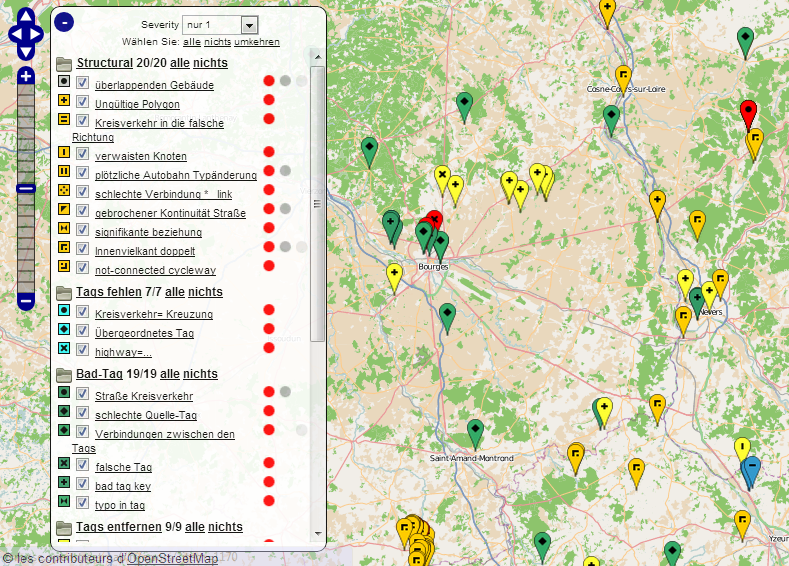
\includegraphics[scale=0.4]{images/managementsummary/osmose-screenshot}
	\caption{Anzeige von Fehlern in Osmose}
	\label{image-osmose-screenshot}
\end{figure}

Andere Lösungen setzen darauf, dass Fehler manuell von einer Person erfasst werden. Dadurch ist es möglich, den Fehler detaillierter zu beschreiben. 
So gibt es Navigationsgeräte-Hersteller, welche die Daten aus \brand{OpenStreetMap} zur Routenberechnung verwenden, und dabei ihren Benutzern ermöglichen, falsche Routen zu melden.

Falls ein \gls{Mapper} einen Fehler melden will, so kann er diesen direkt in den Metadaten der Karte hinterlegen. Alle Objekte auf der Karte (Punkte, Wege und Relationen) können durch beliebige, sogenannte  \glspl{Tag} ergänzt werden.
Um auf einem Objekt Fehler zu markieren, hat sich die Community darauf geeinigt, dafür \inlinecode{FIXME}-\glspl{Tag} zu verwenden.

Quellen für derartige Fehler sind beispielsweise \brand{OpenStreetBugs}\footnote{\url{http://openstreetbugs.schokokeks.org/}} oder die \inlinecode{FIXME}-\glspl{Tag} aus \brand{KeepRight}.

\section*{Ergebnisse}
Das Ziel, eine plattformübergreifende \gls{WebApp} zu erstellen mit geeignetem Backend für die Verwaltung der Daten, wurde klar erreicht.
Die App \kort{} bietet alle Grundfunktionalitäten, welche nötig sind, um Fehler anzuzeigen, zu lösen und gegebene Vorschläge zu validieren.
Daneben sind einige Elemente der \gls{Gamification} implementiert. So ist es beispielsweise möglich, durch das Lösen von Fehlern Punkte (sogenannte \emph{Koins}) zu sammeln und sich über eine Highscore mit anderen Spielern zu messen.
Zudem gibt es für speziellen Einsatz Auszeichnungen zu gewinnen.

\begin{figure}[H]
	\centering
	
\includegraphics[scale=0.6]{images/gamification/gamification-badges}
	\caption{Auszeichnungen in \kort{}}
	\label{image-kort-badges}
\end{figure}

Der Bereich der \gls{Gamification} ist aber sehr offen und lässt Raum für viele weitere Konzepte. Schlussendlich ist jedoch klar, dass \kort{} noch ein Stück davon entfernt ist, ein "`echtes"' Game zu sein.

Das Themengebiet der \gls{Gamification} bietet viele Ansätze, um repetitive Aufgaben spannend zu gestalten.
Gerade bei der Qualitätssicherung von \brand{OpenStreetMap} fallen viele solcher Aufgaben an.
Um die Wahrscheinlichkeit zu erhöhen, dass diese gelöst werden, braucht es neue Werkzeuge, die einfach zu bedienen sind und Spass machen.

\subsection*{Frontend}
Das Frontend basiert auf dem HTML5/JavaScript Framework \brand{Sencha Touch 2} und orientiert sich vom Look and Feel an einer iPhone-App.
Die App bietet für die verschiedenen Funktionen unterschiedliche Tabs an, in welchen der Benutzer Fehler beheben oder prüfen und die Rangliste oder sein Profil anschauen kann.

\begin{figure}[H]
\subfigure{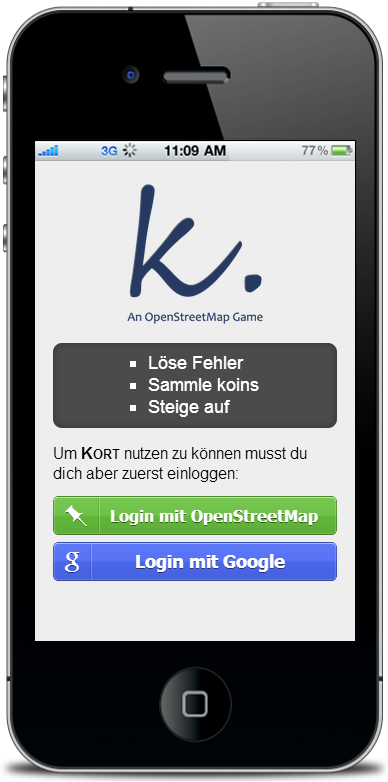
\includegraphics[width=0.3\textwidth]{images/screenshots/kort-screenshot-login}}
\hfill
\subfigure{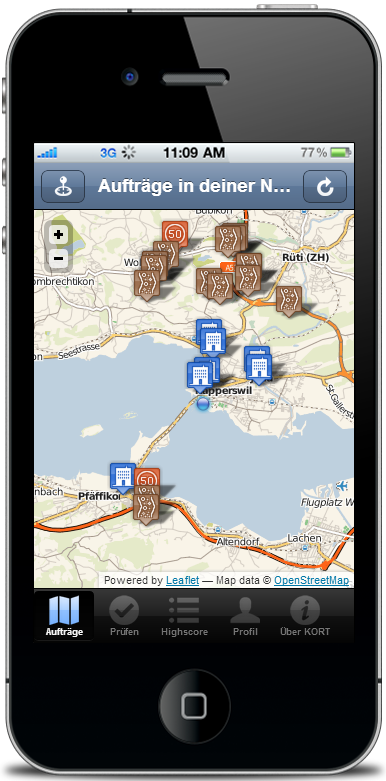
\includegraphics[width=0.3\textwidth]{images/screenshots/kort-screenshot-bugmap}}
\hfill
\subfigure{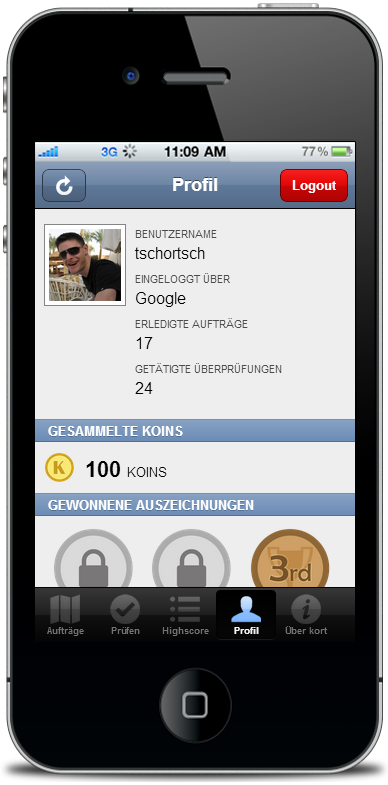
\includegraphics[width=0.3\textwidth]{images/screenshots/kort-screenshot-profile}}
\caption{\kort{} App}
\label{image-kort-screenshots}
\end{figure}

Für die Authentifizierung kommt \gls{OAuth} zum Einsatz.
Der Standard sorgt dafür, dass sich der Benutzer mit einem bereits bestehenden Benutzerkonto bei \kort{} anmelden kann.
Derzeit werden dafür die \gls{OAuth}-Provider \brand{OpenStreetMap} und \brand{Google} verwendet.

\subsection*{Backend}
Das Backend ist in PHP geschrieben und basiert auf der Kommunikation über \gls{REST}-Schnittstellen.
Die eigenen Schnittstellen sind alle mit dem \brand{Slim-Framework}\footnote{\url{http://www.slimframework.com/}} erstellt.
Da die Datenbank und der Webserver auf zwei verschiedenen Servern laufen, bietet auch die Datenbank eine \gls{REST}-Schnittstelle an, über welche sich beliebige SQL-Abfragen absetzen lassen.
Diese flexible Aufteilung ermöglicht es sehr einfach, die Systeme zu migrieren oder weitere hinzuzufügen.

\cleardoublepage
\section*{Ausblick}
Die App hat grosses Potential, Personen, welche sich bislang nicht mit der Thematik \brand{OpenStreetMap} befasst haben, für das Projekt zu begeistern.

Ganz allgemein ist es wichtig, die Robustheit und Geschwindikeit der App zu verbessern. 
Gerade weil es sich um eine \gls{WebApp} handelt, ist dies besonders kritisch. 
Im Idealfall sollte sich die App nicht von einer nativen App unterscheiden.
Es ist zu prüfen, ob es sich lohnt, die App native zu builden\footnote{z.B. mit Apache Cordova oder Sencha Packager}.
Dies hätte den Vorteil, dass die App über die bekannten \glspl{App-Store} zum User gebracht werden kann.

Beim Login wäre es wünschenswert, noch weitere \gls{OAuth}-Dienste anzubieten, um so weitere Personen anzusprechen und die Akzeptanz zu steigern.
Schliesslich verfügt nicht jeder über ein \brand{OpenStreetMap}- oder ein Google-Konto.
Mögliche Dienste sind beispielweise Facebook oder Twitter, welche beide \gls{OAuth} anbieten.

Um die Validierung von Lösungsvorschlägen zu verbessern, wäre es wünschenswert wenn ein Benutzer direkt einen Fotobeweis anbringen könnte.
Dies hilft die Datenqualität hoch zu halten und macht eine Änderung leichter überprüfbar.
Der Benutzer könnte dafür beispielsweise mit zusätzlichen Punkten belohnt werden.
Technisch wäre es sicher spannend sich mit dem \gls{Camera API} auseinander zu setzen.

Als zusätzliche Motivation könnten zeitlich begrenzte Aktionen durchgeführt werden.
Dies soll Benutzer dazu animieren, die App immer wieder zu verwenden. 
Mögliche Aktionen wären beispielsweise die Konzentration auf einen Fehlertyp (\emph{"`Gib allen Restaurants in deiner Umgebung einen Namen und erhalte diese Woche die spezielle Restaurant-Auszeichnung"'}) oder auf eine Region (\emph{"`Korrigiere jeden Tag im Dezember Fehler in Zürich und erhalte die Zürich-Silvester-Auszeichnung"'}).
Die Spieler könnten beispielsweise mittels Push-Notifikationen über solche Aktionen oder sonstige Neuerungen informiert werden.

Um die App längerfristig am Laufen zu halten, ist es unumgänglich, weitere Fehlertypen und -quellen einzubinden. 
\brand{KeepRight} bietet zwar eine grosse Menge an Fehlerdaten, jedoch ist nur ein geringer Teil davon für unsere App nutzbar.

Die Bekanntheit der App muss durch geeignete Massnahmen gesteigert werden. Dazu gehört die Integration von Social Media-Diensten wie Facebook und Twitter.
Diese kann einerseits genutzt werden, um Werbung zu machen, anderseits können Benutzer auf bereits gewonnene Auszeichnungen aufmerksam gemacht werden und so dazu animieren, diese Auszeichnungen ebenfalls zu gewinnen.
Ähnlich wie man es von anderen Apps wie beispielsweise \brand{Foursquare}\footnote{\url{https://foursquare.com/}} oder \brand{SBB.Connect}\footnote{\url{http://www.sbb.ch/fahrplan/mobile-fahrplaene/mobile-apps/sbb-connect.html}} kennt.

Die wichtigste, noch offene Erweiterung stellt aber das noch fehlende Zurückschreiben der eingetragenen Lösungen zu \brand{OpenStreetMap} dar.
Diese Funktionalität wirkt sich stark auf die Akzeptanz der App seitens der \brand{OpenStreetMap}-Community aus.

% Inhaltsverzeichnis
\tableofcontents

% -----------------------------------------
% BODY
% -----------------------------------------
% Neue Seite beginnen (um Seitennummerierung zurückzusetzen)
\cleardoublepage

% Seitennummerierung mit arabischen Zeichen
\pagenumbering{arabic}

% Einführung
% Titel auch in Kopfzeile anzeigen
\markboth{Teil I. Einführung}{Teil I. Einführung}
\part{Einführung}
% Informationen zum Projekt
\chapter{Informationen zum Projekt}
\label{informationen-projekt}


\section{Problemstellung}
\brand{OpenStreetMap} (OSM) ist ein freies Projekt, welches jedermann ermöglicht, Kartendaten anzuzeigen und zu editieren.
Durch diesen öffentlichen Charakter ist es nicht ausgeschlossen, dass fehlerhafte bzw. unvollständige Daten eingetragen werden.

Aus diesem Grund entstand die Idee, mit einer mobilen Applikation eine Möglichkeit anzubieten, Fehler auf einfache Weise anzuzeigen und zu korrigieren.
Um die Motivation für die Verwendung der App längerfristig aufrecht zu erhalten, soll diese mit Spiel-Elementen versehen werden.

\section{Aufgabenstellung}
Im Rahmen dieser Arbeit wird eine HTML5 \gls{WebApp} entwickelt, welche es ermöglicht, unvollständige bzw. fehlerhafte Daten in der \brand{OpenStreetMap}-Datenbank zu korrigieren oder zu vervollständigen.

Die App soll nicht als herkömmlicher Editor implementiert werden, sondern einen gewissen Gamecharakter aufweisen.
Dieser zeichnet sich dadurch aus, dass die Benutzer für ihre Änderungsvorschläge belohnt werden.
So können sie beispielsweise in der Rangliste (Highscore) aufsteigen oder Auszeichnungen (Badges) gewinnen.
Dieses Konzept ist unter dem Stichwort \gls{Gamification} bekannt.
Damit ist allgemein die Anwendung von Spiel-Elementen in einem spielfremden Kontext gemeint.
Es soll untersucht werden, ob und wie sich dies für \brand{OpenStreetMap} umsetzen lässt.

Eingetragene Änderungsvorschläge können anschliessend von weiteren Benutzern kontrolliert und bewertet werden.
Mehrfach validierte Änderungen sollen ins \brand{OpenStreetMap}-Projekt zurückgeführt werden.

Mit der Integration von Social Media-Diensten (Facebook, Twitter) soll die Bekanntheit der App gefördert und die Motivation der Benutzer gesteigert werden.

\cleardoublepage
\section{Ziele}
In der Aufgabenstellung der Arbeit wurden folgende Ziele definiert:
\begin{itemize}
	\item Erstellen einer cross-platform HTML5 \gls{WebApp} mit JavaScript
	\item Einsatz von JavaScript-\glspl{API} zur Ansteuerung von Hardwarekomponenten (z.B. GPS, Kamera)
	\item Es soll geprüft werden, ob die \gls{WebApp} auch als native App für die Plattformen iOS und Android zur Verfügung gestellt werden kann 
	\item Als Basis sollen Daten und Webdienste des \brand{OpenStreetMap}-Projekts verwendet werden
	\begin{itemize}
		\item Quellen für bekannte Fehler: \brand{OpenStreetMap} Bug Reports, \inlinecode{FIXME}- und \inlinecode{TODO}-\glspl{Tag}
		\item Unterstützung von \gls{POI}-, Linestring- und Polygon-Objekten
	\end{itemize}
	\item Verwendung einer vorhandenen User-Basis für die Authentifizierung (\gls{OAuth})
	\item Integration von Social Media zum Austausch von Aktivitäten
	\item Konzept für Gamification von \brand{OpenStreetMap} erarbeiten
	\begin{itemize}
		\item Highscores / Rankings
		\item Badges / Achievements
		\item Aufgaben mit verschiedenen Schwierigkeitsstufen
	\end{itemize}
	\item Verschiedene Modi
	\begin{itemize}
		\item Erfassen von Daten, Aufnahme von Fotos (ortsbezogen)
		\item Verifikation von eingegebenen Daten (ortsunabhängig)
	\end{itemize}
	\item Das User Interface soll primär auf Deutsch erstellt werden. Es sollen jedoch Vorkehrungen getroffen werden, um Übersetzungen einfach zu ermöglichen (Internationalisierung)
\end{itemize}

\section{Rahmenbedingungen}
\begin{itemize}
\item Es gelten die Rahmenbedingungen, Vorgaben und Termine der HSR
\item Die Projektabwicklung orientiert sich an einer iterativen, agilen Vorgehensweise. Als Vorgabe dient dabei Scrum, wobei bedingt durch das kleine Projektteam gewisse Vereinfachungen vorgenommen werden.
\item Die Kommunikation in der Projektgruppe, in der Dokumentation und an den Präsentationen erfolgt auf Deutsch.
\end{itemize}

\section{Aufbau der Arbeit}
Die Arbeit ist in drei Teile gegliedert. Im ersten Teil erfolgt eine Einleitung mit allgemeinen Informationen zum Projekt und dessen Umsetzung (siehe Kapitel \ref{informationen-projekt}. Informationen zum Projekt, \ref{umsetzung}. Umsetzung und \ref{kort-definitionen}. Definitionen). Darin werden auch Begriffe erklärt, welche während der Arbeit entwickelt oder oft verwendet werden.

Der zweite Teil beinhaltet die Dokumentation der eigentlichen Arbeitsresultate (siehe Kapitel \ref{kort}. Kort, \ref{leaflet-sencha-komponente}. Leaflet Komponente, \ref{gamification}. Gamification, \ref{datenquellen}. Datenquellen, \ref{architektur}. Architektur, \ref{infrastruktur}. Infrastruktur, \ref{backend}. Backend und \ref{administration}. Administration). Darin wird unter anderem die Implementation der \gls{WebApp} beschrieben und die Infrastruktur, welche für den Betrieb notwendig ist.

Im dritten Teil befinden sich Informationen zum Projektmanagement (siehe Kapitel \ref{projektmanagement}. Projektmanagement und \ref{projektmonitoring}. Projektmonitoring).

Neben diesem Dokument umfasst die Arbeit die implementierte \gls{WebApp} \kort{}. Der dazugehörige Source Code ist frei im Internet zugänglich, sowie auf der beigelegten CD zu finden.

\begin{table}[H]
\centering
\begin{tabular}{|p{0.3\twocelltabwidth}|p{0.7\twocelltabwidth}|}
\hline 
\textbf{Arbeitsresultat} & \textbf{URL} \\ 
\hline 
\kort{} (\gls{WebApp}) & \url{http://kort.herokuapp.com} \\ 
\hline 
Repository & \url{https://github.com/odi86/kort} \\ 
\hline 
\end{tabular}
\label{arbeitsresultate}
\caption{Übersicht der Arbeitsresultate}
\end{table} 

% Umsetzung
\chapter{Umsetzung}
\label{umsetzung}

\section{Stand der Technik}
Da es sich bei \brand{OpenStreetMap} um ein globales Projekt handelt, gibt es zahlreiche Anstrengungen, die Karte besser zu machen.
Neben konventionellen Editoren gibt es auch Tools, welche sich explizit auf das Finden und Beheben von Fehlern spezialisiert haben.
Ein Beispiel dafür ist der \brand{NoName-Layer} von Simon Poole\footnote{\url{http://wiki.openstreetmap.org/wiki/NoName}}. Dieser färbt Strassen, welche fälschlicherweise keinen Namen haben, rot ein.
Daneben gibt es Dienste, welche Fehlerdaten sammeln und diese zur Verbesserung anbieten, wie beispielsweise \brand{KeepRight}\footnote{\url{http://www.keepright.at/}} oder \brand{OpenStreetBugs}\footnote{\url{http://openstreetbugs.schokokeks.org/}}.

Die Gemeinsamkeit dieser Werkzeuge liegt darin, dass sie vom Benutzer bereits ein gewisses Interesse an \brand{OpenStreetMap} und am Editieren der Karte voraussetzen.
Karten-Fehler sind jedoch typische Beispiele, welche sich durch die Mithilfe von möglichst vielen Personen lösen lassen (sogenanntes \emph{\gls{Crowdsourcing}}).
Die Voraussetzung für ein erfolgreiches \gls{Crowdsourcing} ist, möglichst viele Hürden abzubauen und einfach zu lösende Aufgaben bereit zu stellen.
Das Konzept der \gls{Gamification} bietet sich daher an.

Dabei werden Spiel-Elemente in eine Applikation eingebaut und dadurch die Motivation der Benutzer gesteigert, diese Applikation längerfristig zu verwenden.
Es gibt bereits einige Projekte, welche sich mit der \gls{Gamification} von \brand{OpenStreetMap} beschäftigen\footnote{\url{http://wiki.openstreetmap.org/wiki/Games\#Gamification_of_map_contributions}}.

\brand{MapRoulette}\footnote{\url{http://wiki.openstreetmap.org/wiki/MapRoulette}} stellt dem Benutzer eine \emph{Challenge}, welche es zu lösen gibt.
Ein Beispiel einer solchen Challenge ist \emph{Connectivity}\footnote{\url{https://oegeo.wordpress.com/2012/10/29/new-maproulette-challenge-connectivity-bugs/}}, bei welcher Strassen, die sehr nahe beieinander liegen verbunden werden sollen.
Der Benutzer hat die Wahl, ob er den Fehler korrigiert, ignoriert oder als \emph{false positive} markiert.
Wenn der Benutzer einen Fehler gelöst hat, wird ihm zufällig ein weiterer Fehler angezeigt.
Die Challange ist dann fertig, wenn alle Fehler einer Kategorie behoben sind.
Durch die Weiterleitung auf den nächsten Fehler entsteht ein beinahe endloses Spiel. Jede erledigte Aufgabe hat dabei den Charakter eines Levels.

Im Rahmen der \emph{Operation Cowboy}\footnote{\url{http://wiki.openstreetmap.org/wiki/DE:Operation_Cowboy}} wurden unter anderem auch mit \brand{MapRoulette} über 2000 \gls{Routing}-Fehler pro Tag behoben\footnote{\url{https://twitter.com/opcowboy/status/272438199769501696}}.

\section{Vision}
Die \gls{WebApp} \kort{} bietet dem Benutzer eine einfache Oberfläche, Fehler zu lokalisieren.
Das Zielpublikum hat keinerlei Vorwissen über Karten oder \brand{OpenStreetMap}.
Da die App als Spiel konzipiert ist, werden dem Benutzer kleine, einfach zu lösende Aufgaben gestellt.
Diese Aufgaben beziehen sich auf Fehler in den Karten-Daten.

Für das Lösen solcher Aufgaben gewinnt der Benutzer Punkte und kann so in der Highscore aufsteigen.
Für besondere Leistungen werden ihm dabei auch Auszeichnungen verliehen.
Dieser Mix sorgt dafür, dass der Benutzer die App immer wieder öffnet, um weitere Korrekturen vorzunehmen.

Als Alternative zum Beantworten von Fragen, hat der Benutzer die Möglichkeit, die Antworten von anderen Spielern zu validieren.
Dazu soll er die gegebenen Antworten als richtig oder falsch markieren.
Erreicht eine Antwort genügend Stimmen, welche deren Richtigkeit bestätigen, gilt diese als abgeschlossen und kann anschliessend als Korrektur an \brand{OpenStreetMap} gesendet werden.

Durch die Implementation als cross-platform \gls{WebApp}, kann diese auf allen gängigen mobilen Betriebssystemen verwendet werden.

\section{Resultate der Arbeit}
Wir konnten fast alle gesetzten Ziele erreichen.
\kort{} erfüllt alle Anforderungen an eine moderne \gls{WebApp}.
Nach dem Login über \gls{OAuth} werden dem Benutzer Fehler in seiner Umgebung auf der Karte angezeigt.

Um das Spiel zu starten, kann der Benutzer eine beliebige Aktionen durchführen.
Wenn er beispielsweise einen Fehler auswählt, indem er auf dessen Markierung tippt, wird er gefragt, ob er die Lösung für den Fehler kennt.
Dadurch soll die Neugier des Spielers geweckt werden.

Die Spielmechanik ist denkbar einfach, so dass das Spiel auch nur sekunden-, aber auch  minutenlang gespielt werden kann.
Der Benutzer erhält sofort ein Feedback und kann verfolgen, wie er sich gegenüber seinen Mitspielern verbessert.
Eine zusätzliche Motivation wird über Auszeichnungen geschaffen.

Wir konnten einige Gamificationkonzepte direkt in der App umsetzen.
Um das Spiel für möglichst viele Benutzer attraktiv zu machen, muss aber noch ein detaillierteres Konzept ausgearbeitet werden.
Gerade mit den Badges lassen sich verschiedene Spielertypen ansprechen.
Auch Schwierigkeitsstufen oder zusätzliche Berechtigungen für erfahrene Benutzer können den längerfristigen Erfolg der Applikation erhöhen.

Auf der technischen Seite haben wir erfolgreich ein System entwickelt, welches stets mit neuen Fehlern "`gefüttert"' wird.
Die Architektur ist so flexibel gewählt, dass sich beinahe beliebig Komponenten hinzufügen oder entfernen lassen.
Dies stellt sicher, dass zukünftig auch weitere Fehlerdatenquellen in \kort{} integriert werden können.

\section{Schlussfolgerungen und Ausblick}
Einige Punkte aus der Aufgabenstellung sind noch offen.
Wir hatten das Ziel, dass Benutzern neben einer textuellen Antwort auch noch ein Bild hochzuladen können, quasi als Beweis für ihre eingetragene Fehlerkorrektur.
Dabei sind wir jedoch an einer technischen Limite des verwendeten Frontend-Frameworks \brand{Sencha Touch 2} gescheitert.
Des weiteren sollten soziale Medien wie Facebook und Twitter integriert werden, um eine breitere Öffentlichkeit zu erreichen.
Im Verlaufe der Arbeit haben sich die Prioritäten diesbezüglich aber geändert.

Als letzter offener Punkt bleibt noch das Zurückschicken der Korrekturen zu \brand{OpenStreetMap}.
Da wir damit beschäftigt waren unser eigenes System fertig zu stellen, konnten wir dies schlussendlich aus Zeitgründen nicht mehr implementieren.

Die App in der jetzigen Form ist also in sich geschlossen. Die getätigten Korrekturen werden in der eigenen Datenbank abgelegt, jedoch noch nicht zu \brand{OpenStreetMap} zurückgesendet.

Wir mussten in dieser Arbeit feststellen, dass zuerst viele Grundfunktionen implementiert werden müssen, auf denen dann Weiterentwicklungen stattfinden können.
Ursprünglich haben wir uns erhofft, tiefer in die Thematik der \gls{Gamification} einzusteigen und die App als "`echtes"' Game zu gestalten.

Wenn unsere App trotzdem mithelfen kann, einzelne Benutzer für das \glslink{Mapper}{Mappen} zu begeistern, haben wir unser Ziel jedoch mehr als erreicht.

% Begriffsdefinitionen
\chapter{Begriffsdefinitionen}
\label{kort-definitionen}

Für diese Arbeit wurden einige neue Begriffe verwendet und Konzepte definiert.
Dieses Kapitel soll kurz die wichtigsten Begriffe von \kort{} erklären.
Hierbei handelt es sich um fachliches Vokabular, welches in dieser Arbeit verwendet wird.
Alle anderen, eher technischen Begriffe, befinden sich im Glossar (siehe Teil \ref{glossar}).

\section{Name der Applikation}
Beim Begriff \kort{} handelt es sich um einen skandinavischen Ausdruck für \emph{Karte}.
Obwohl dieser Begriff sehr allgemein ist, scheint er im Zusammenhang mit Applikationen noch nicht häufig verwendet worden zu sein.
Der Name ist kurz und prägnant, was für eine App ideal ist.

Falls die App zukünftig auch im skandinavischen Raum verwendet wird, muss eine Namensänderung allfällig in Betracht gezogen werden.

\section{Begriffe aus dem Spiel}

\begin{table}[H]
\centering
\begin{tabular}{|p{0.2\threecelltabwidth}|p{0.12\threecelltabwidth}|p{0.68\threecelltabwidth}|}
\hline 
\small{\textbf{Kategorie}} & \small{\textbf{Begriff}} & \small{\textbf{Beschreibung}} \\
\hline 
Spieleinheit & Auftrag & Aufträge sind Fehler auf der Karte, welche von einem Benutzer korrigiert werden. \\
\hline 
Belohnung & Koins & Punkte, welcher ein Benutzer gewinnen kann, werden \emph{Koins} genannt.
Das Wort ist vom Englischen \emph{coin} (Münze) abgeleitet. 
Das "`K"' ist dabei eine Anlehnung an den Spielnamen \kort{}. \\
\hline 
Auszeichnungen & Badge & Auszeichnungen, die ein Benutzer gewinnen kann, werden \emph{Badge} genannt. \\
\hline 
Rangliste & Highscore & Rangliste aller Spieler, sortiert nach Anzahl \emph{Koins}. \\
\hline 
Punkt auf der Karte & Objekt & Ein speziell ausgezeichneter Ort (\gls{POI}) auf der Karte, zu dem Informationen fehlen. \\
\hline 
\end{tabular}
\caption{Begriffe aus \kort{}}
\label{table-definitionen}
\end{table}

% Neue Seite beginnen
\cleardoublepage

% Projektdokumentation
% Titel auch in Kopfzeile anzeigen
\markboth{Teil II. Projektdokumentation}{Teil II. Projektdokumentation}
\part{Projektdokumentation}
% Frontend
\chapter{Kort}
\label{kort}

\begin{center}
\begin{figure}[H]
\begin{center}
\subfigure{
\includegraphics[scale=0.8]{images/implementation/frontend/kort-icon_with_gloss}}
\hspace{1cm}
\subfigure{
\includegraphics[scale=0.8]{images/implementation/frontend/kort_herokuapp_com-qrcode}}
\end{center}
\end{figure}

{\Large \textbf{\url{http://kort.herokuapp.com/}}}

\vspace{1cm}

\begin{figure}[H]
\subfigure{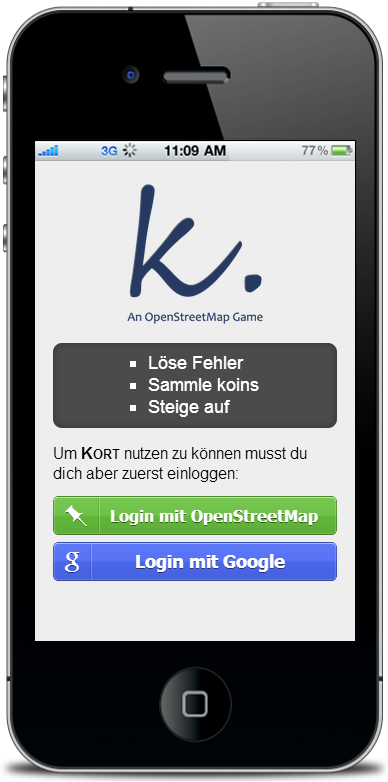
\includegraphics[width=0.3\textwidth]{images/screenshots/kort-screenshot-login}}
\hfill
\subfigure{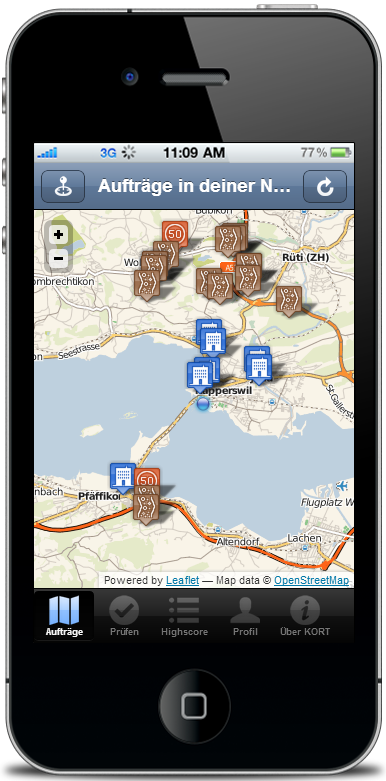
\includegraphics[width=0.3\textwidth]{images/screenshots/kort-screenshot-bugmap}}
\hfill
\subfigure{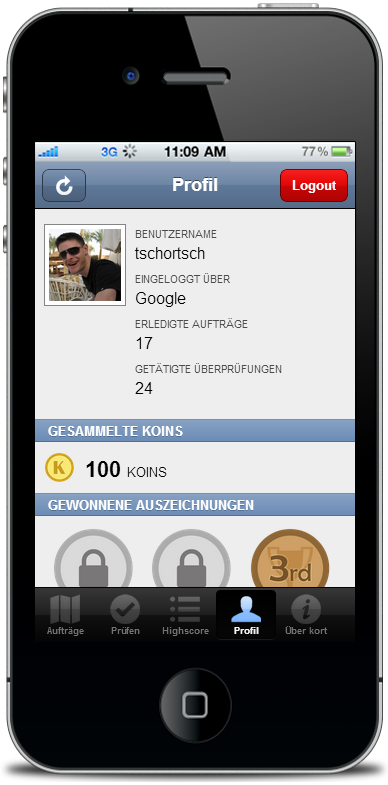
\includegraphics[width=0.3\textwidth]{images/screenshots/kort-screenshot-profile}}
\end{figure}
\end{center}

% Analyse
% Analyse
\section{Analyse}

% User Szenarien
\subsection{User Szenarien}
\label{kort-user-szenarien}

Um die Anforderungen an die App genauer abschätzen zu können, wurden im Vorfeld der Implementierung einige Szenarien erstellt.

\subsubsection{Szenario 1: Zeitvertreib an der Bushaltestelle}

Simon muss 15 Minuten an der Bushaltestelle auf den nächsten Bus warten.
Um sich die Wartezeit zu verkürzen, nimmt er sein Smartphone hervor und startet die \kort{}-Applikation.

Die App hat ihn bereits lokalisiert und zeigt ihm offene \brand{OpenStreetMap}-Aufträge in der Nähe, wahlweise als Liste oder auf der Karte an.
Für die Aufträge werden Simon verschiedene Belohnungen angeboten, abhängig vom Schwierigkeitsgrad der Aufgabe.

Simon entscheidet sich für einen Auftrag mit mittlerer Belohnung.
Die App zeigt ihm den Weg zum Auftrag und erklärt, was zu tun ist.
Beim Auftrag handelt es sich um einen fehlenden Strassennamen.

Als Simon vor Ort ist, findet er sehr schnell ein Strassenschild.
Er gibt den Namen in der App ein wofür er bereits 10 Punkte erhält.
Da er zusätzlich sogar noch ein Foto hochlädt, bekommt er weitere 5 Punkte.

Der Auftrag ist somit für ihn erledigt, was ihm entsprechend von der App mitgeteilt wird.
Danach verschwindet der Auftrag aus seiner Auftragsliste und von der Karte.

\textbf{Ziele}
\begin{itemize}
\item Zeitvertreib
\item Punkte sammeln
\item Daten verbessern
\end{itemize}

\subsubsection{Szenario 2: Validieren}

Andy sitzt im Zug und langweilt sich.
Er öffnet die \kort{}-App im Indoor-Modus und sieht sich die Liste der zu validierenden Lösungsvorschläge an. 
Er sortiert die Liste, um diejenigen Einträge zu sehen, welche nur noch einen Review benötigen, um an \brand{OpenStreetMap} gesendet werden zu können.

Er öffnet einen Vorschlag für einen fehlenden Strassennamen in der Umgebung.
Er kennt zwar die Gegend ist sich aber nicht 100\% sicher ob der Name stimmt.
Um sicherzugehen, öffnet er das angehängte Bild.
Das Bild zeigt ein Strassenschild, welches mit dem eingegeben Namen übereinstimmt
Andy bestätigt dann die Änderung und schliesst den Bug damit ab.

\cleardoublepage
\textbf{Ziele}
\begin{itemize}
\item Schnell und einfach geeignete Einträge zum Validieren finden
\item Qualität der Änderungen sicherstellen
\end{itemize}

\subsubsection{Szenario 3: Erster Kontakt zur App}

Über den Kurznachrichtendienst Twitter sieht Monika, dass ihre Kollegin gerade das erste mal \kort{} gestartet hat.
Als sie auf den Link klickt öffnet sich ihr Browser und die App wird angezeigt.
Da es sich um ihren ersten Besuch auf der Seite handelt, wird ihr kurz erklärt um was es geht.

Danach sieht sie die Karte mit den vorhandenen Fehlereinträgen.
Bevor sie einen Eintrag bearbeiten kann, muss sie sich anmelden.
Sie wählt dazu einen Benutzernamen und wird anschliessend auf die Seite von Google weitergeleitet, um sich anzumelden.
Nach dem erfolgreichen Login wird Monika zurück zur \kort{}-App geleitet, wo sie beginnen kann, die ersten Aufträge zu erfüllen.

\textbf{Ziele}
\begin{itemize}
\item Direkt ersichtlich, was die App kann
\item Schneller Einstieg
\item Einfache Anmeldung (keine Registrierung!)
\item Benutzerführung durch die Funktionen
\end{itemize}

\subsubsection{Szenario 4: Highscore-Anwärter}

Edi benutzt schon seit einiger Zeit die \kort{}-App und hat in seinem Revier bereits den zweiten Platz der Highscore erreicht.
Seine Platzierung überprüft er regelmässig in der App.

Heute möchte er endlich die Spitze erklimmen und den "`Leader"'-Badge erhalten.
Dazu hat er sich einige Aufträge ausgesucht, welche er der Reihe nach bearbeiten will.
Bei jedem Auftrag sieht Edi, wie viele Punkte er sammeln kann.

Nachdem er den 5. Auftrag erfolgreich erledigt hat, erhält er eine Benachrichtigung, dass er den "`Leader"'-Badge erhalten hat.
Auch in der Rangliste steht Edi nun zuoberst.

\textbf{Ziele}
\begin{itemize}
\item Einfach mehrere Aufträge nacheinander ausführen
\item Badges sammeln
\item Highscore anzeigen
\item Erster Rang erreichen
\end{itemize}

% Paper-Prototype
\subsection{Paper-Prototype}
% Subfigure counter zuruecksetzen
\setcounter{subfigure}{0}

Aus den gesetzten Projektzielen und den Anforderungen der erstellten Szenarien (siehe Abschnitt \ref{kort-user-szenarien}) wurde vor der Implementation der Oberfläche ein Paper-Prototype des GUI-Designs erstellt.
Der Prototype besteht aus vier Hauptmasken und einem Overlay für den Login.

\subsubsection{Overlay: Login}
Beim ersten Starten der \gls{WebApp} erhält man die Möglichkeit sich über verschiedene Dienste anzumelden.
Mit einem Klick auf den jeweiligen Anbieter, wird man zu diesem weitergeleitet und kann sich dort anmelden.

\begin{figure}[H]
\subfigure[Login - Anbieterauswahl]{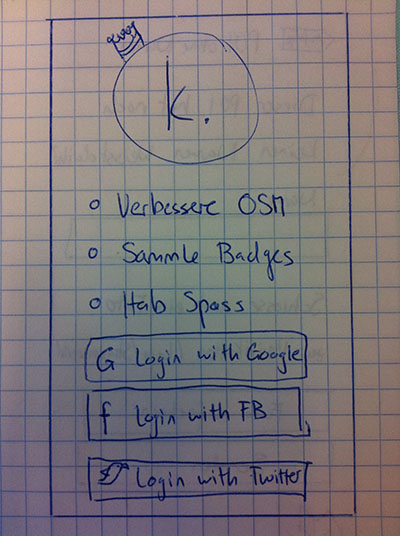
\includegraphics[width=0.43\textwidth]{images/paperprototype/kort-pp-startscreen}}
\hfill
\subfigure[Login - Loginformular des jeweiligen Anbieters]{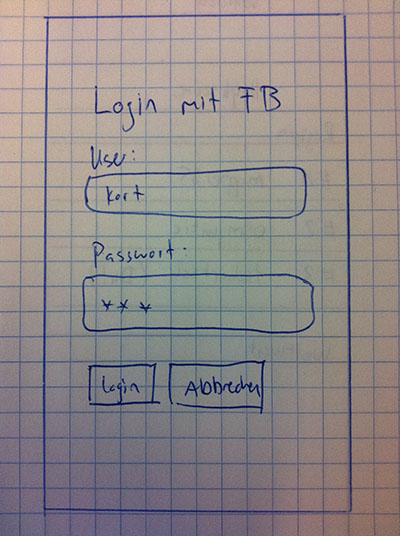
\includegraphics[width=0.43\textwidth]{images/paperprototype/kort-pp-login}}
\end{figure}

\cleardoublepage
\subsubsection{Maske: Aufträge}
Nachdem sich der Benutzer erfolgreich angemeldet hat, erscheint die Maske mit den Aufträgen.
Darauf werden die vorhandenen Fehler auf einer Karte angezeigt.
Es werden jeweils nur die Fehler angezeigt, welche sich in unmittelbarer Nähe des eigenen Standorts befinden.
Die Fehler werden mit einer Markierung auf der Karte dargestellt.

Durch Anklicken einer solchen Markierung öffnet sich die Detailansicht des Fehlers, wo sich der Fehler direkt beheben lässt.
Neben der Möglichkeit, einen Lösungstext einzugeben, soll es auch möglich sein, ein Beweis-Foto hochzuladen.
Mit einem Klick auf den Senden-Knopf schliesst sich die Detailansicht und man gelangt zur Karte mit den Aufträgen zurück.

\begin{figure}[H]
\subfigure[Aufträge - Karte mit Fehlern]{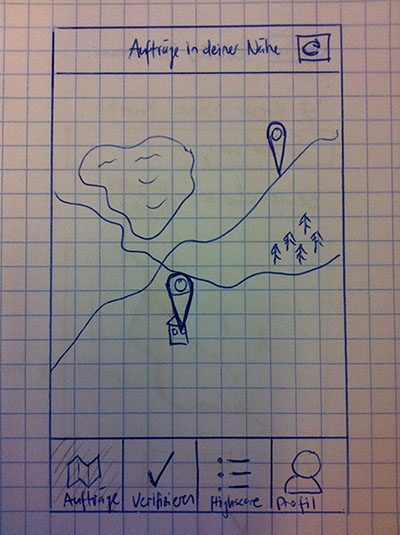
\includegraphics[width=0.43\textwidth]{images/paperprototype/kort-pp-bugs}}
\hfill
\subfigure[Aufträge - Detailansicht eines Fehlers]{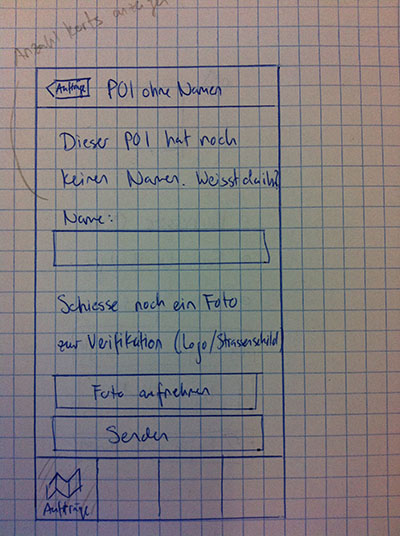
\includegraphics[width=0.43\textwidth]{images/paperprototype/kort-pp-fix}}
\end{figure}

\cleardoublepage
\subsubsection{Maske: Verifizieren}
Auf der Verifikationsmaske werden die bereits gelösten Fehler in der Nähe angezeigt.
Sie sind gruppiert nach Anzahl nötigen Verifikationen, um sie an \brand{OpenStreetMap} zurückzusenden.

Per Klick auf einen Eintrag öffnet sich die Verifikationsmaske.
Darin wird der Fehlerlösungstext und das Beweis-Foto angezeigt.
Zusätzlich wird das betroffene \brand{OpenStreetMap}-Objekt auf einer Karte angezeigt.
Man hat die Möglichkeit, die Problemlösung als \emph{Korrekt} oder \emph{Falsch} zu bewerten.

\begin{figure}[H]
\subfigure[Verifizieren - Liste mit Fehlerlösungen]{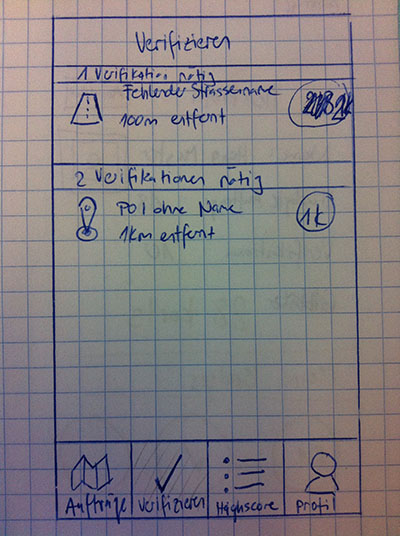
\includegraphics[width=0.43\textwidth]{images/paperprototype/kort-pp-verify}}
\hfill
\subfigure[Verifizieren - Detailansicht einer Fehlerlösung]{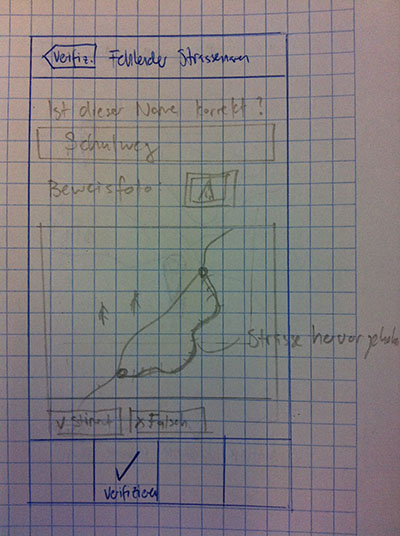
\includegraphics[width=0.43\textwidth]{images/paperprototype/kort-pp-verify_detail}}
\end{figure}

\cleardoublepage
\subsubsection{Maske: Highscore}
In der Highscore-Maske kann man sich mit anderen Spielern messen.
Man sieht seine eigene Platzierung und die der anderen Spieler.
Es werden Highscores für verschiedene Kategorien (z.B. regional, weltweit) angezeigt.

\subsubsection{Maske: Profil}
Im Profil werden die Eckdaten des eigenen Benutzers angezeigt.
Dazu gehören die Anzahl der gelösten Aufträge und die Anzahl der getätigten Verifikationen.
Zusätzlich werden die Gesamtanzahl der gesammelten Punkte und die gewonnenen Badges ausgewiesen.
Auf der Profil-Maske kann sich der Benutzer von der App abzumelden.

\begin{figure}[H]
\subfigure[Highscore]{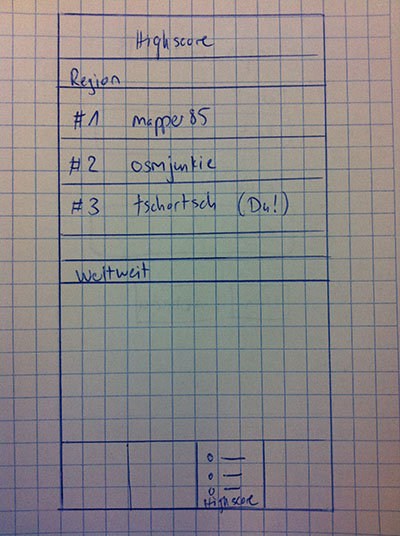
\includegraphics[width=0.43\textwidth]{images/paperprototype/kort-pp-highscore}}
\hfill
\subfigure[Profil]{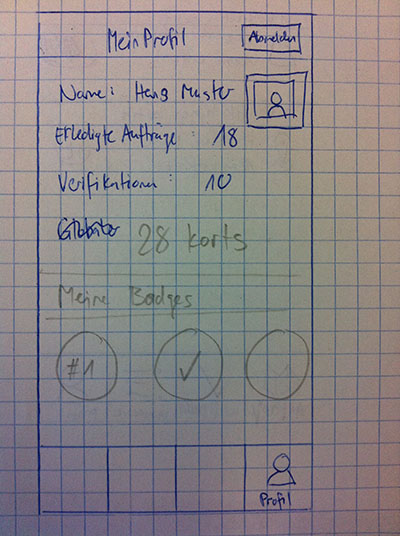
\includegraphics[width=0.43\textwidth]{images/paperprototype/kort-pp-profile}}
\end{figure}

% Design
% Design
\section{Design}

\subsection{Package-Struktur}

Die Package-Struktur wird vom \brand{Sencha Touch 2}-Framework vorgegeben. Sie entspricht grundsätzlich dem \gls{MVC}-Layout.
Speziell daran ist das Konzept der \emph{Stores}, welche einen beliebigen Datenspeicher abstrahieren.
Stores sind an ein \emph{Model} gebunden, welches die Struktur der gespeicherten Daten vorgibt.

Zusätzlich sind sie über einen \emph{Proxy} mit der Datenquelle verbunden.
Dabei kann es sich beispielsweise um einen \gls{REST}-Webservice handeln oder den \gls{Local Storage} des Browsers.

In Abbildung \ref{image-kort-packagediagram} wird die Package-Struktur von \kort{} mit deren Abhängigkeiten gezeigt.

\begin{figure}[H]
	\centering
	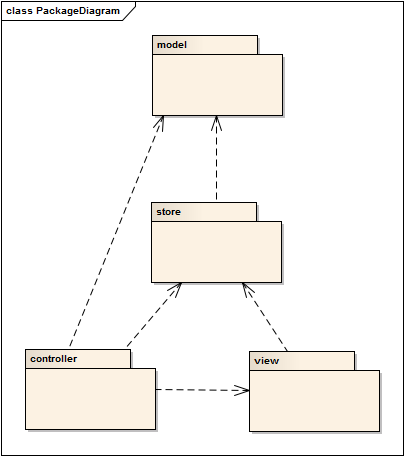
\includegraphics[scale=0.7]{images/uml/kort-packagediagram}
	\caption{Package-Struktur}
	\label{image-kort-packagediagram}
\end{figure}

\subsection{Controller-Package}

Die App ist so gestaltet, dass jede Hauptansicht einen eigenen Controller besitzt.
Dieser ist für die Steuerung der Benutzeroberfläche zuständig.

Die verschiedenen Controller lassen sich grob in drei Klassen einteilen.
Zunächst gibt es Controller für die einzelnen Masken der Applikation (siehe Abbildung \ref{image-kort-classdiagram-controller} $\rightarrow$ \emph{main tab controllers}).
Zusätzlich haben einige Tabs eine Detailansicht, welche ebenfalls von einem eigenen Controller gesteuert wird (siehe Abbildung \ref{image-kort-classdiagram-controller} $\rightarrow$ \emph{detail controllers}).
Zuletzt gibt es eigenständige Controller für die Overlay-Komponenten, welche die gesamte Oberfläche der App verdecken (siehe Abbildung \ref{image-kort-classdiagram-controller} $\rightarrow$ \emph{overlay controllers}).

\begin{figure}[H]
	\centering
	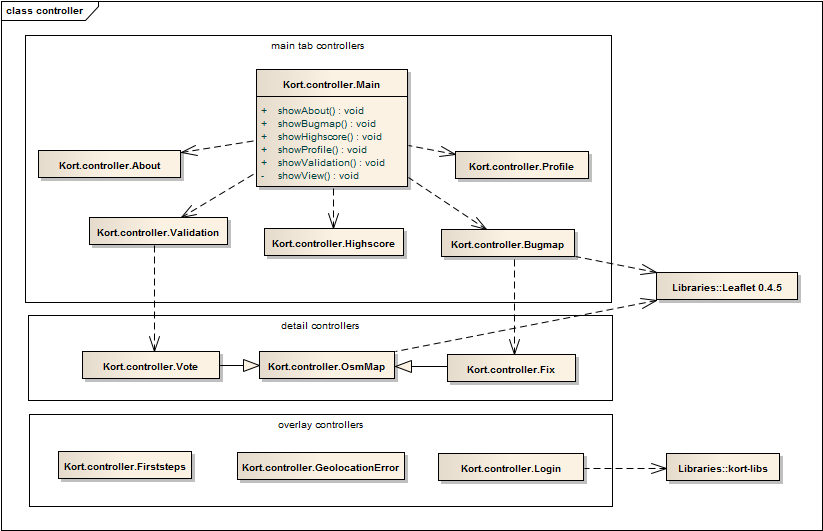
\includegraphics[width=\textwidth]{images/uml/kort-classdiagram-controller}
	\caption{Klassendiagramm der Controller}
	\label{image-kort-classdiagram-controller}
\end{figure}

\subsection{Store- und Model-Package}
\label{kort-store-model-package}

Die \emph{Stores} bilden die Datenspeicher in einer \brand{Sencha Touch} Applikation.
Über ein \emph{Model} wird die jeweilige Struktur der gespeicherten Daten festgelegt.
Stores sind zudem über einen \emph{Proxy} mit der Datenquelle verbunden.
Im Falle von \kort{} wurden dafür ausschliesslich \gls{REST}-Ressourcen verwendet (siehe Abbildung \ref{image-kort-classdiagram-store}).

\begin{figure}[H]
	\centering
	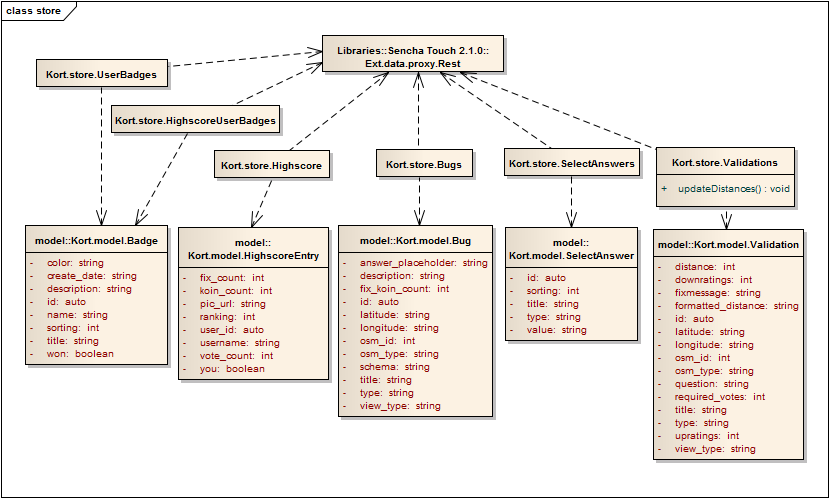
\includegraphics[width=\textwidth]{images/uml/kort-classdiagram-store}
	\caption{Klassendiagramm der Stores}
	\label{image-kort-classdiagram-store}
\end{figure}

\subsubsection{Models ohne Store}

Falls die Applikation jeweils nur eine Instanz eines \emph{Models} verwendet, können diese ohne einen Store direkt mit einem Proxy verbunden werden.
In \kort{} wurde dies für den eingeloggten Benutzer (User) sowie für die zu sendenden Datenpakete wie der Fehler-Lösung (Fix) und der Validierung (Vote) verwendet (siehe Abbildung \ref{image-kort-classdiagram-model_own_proxy}).

\begin{figure}[H]
	\centering
	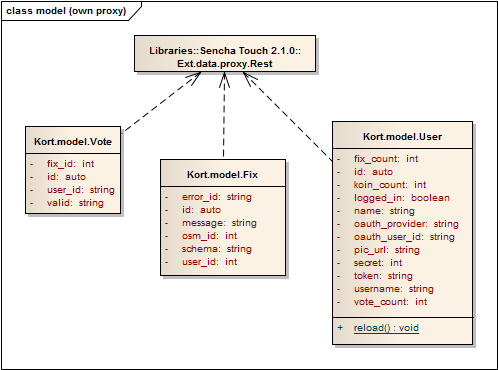
\includegraphics[scale=0.5]{images/uml/kort-classdiagram-model_own_proxy}
	\caption{Klassendiagramm der Models ohne Stores}
	\label{image-kort-classdiagram-model_own_proxy}
\end{figure}

\subsubsection{Speichern der Logininformationen}
Die Logininformationen des Benutzers werden im \gls{Local Storage} des Browsers abgelegt (siehe Abbildung \ref{image-kort-classdiagram-store_localstorage}).
Der genaue Ablauf wird in Abschnitt \ref{oauth} beschrieben.

\begin{figure}[H]
	\centering
	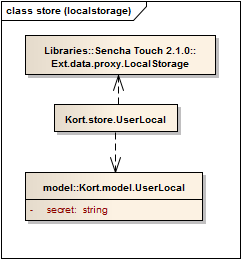
\includegraphics[scale=0.6]{images/uml/kort-classdiagram-store_localstorage}
	\caption{Speichern der Logininformationen im Local Storage}
	\label{image-kort-classdiagram-store_localstorage}
\end{figure}

\subsection{Aufbau der Benutzeroberfläche}
Jede Maske der Applikation befindet sich in einer eigenen View-Klasse.
Diese verschiedenen View-Klassen werden in der Hauptklasse \inlinecode{Kort.view.Main} inkludiert und angezeigt (siehe Abbildung \ref{image-kort-classdiagram-view}).

\begin{figure}[H]
	\centering
	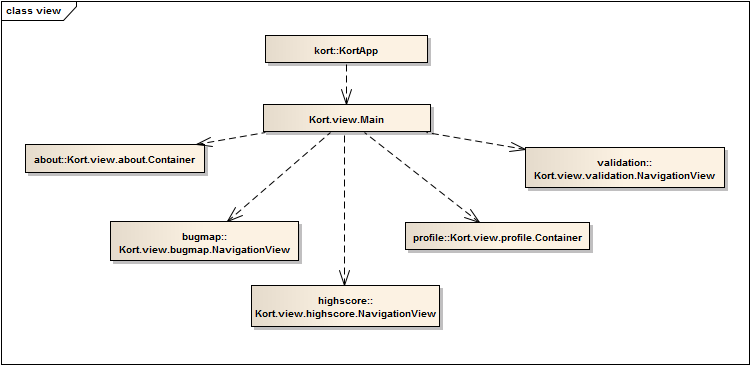
\includegraphics[width=\textwidth]{images/uml/kort-classdiagram-view}
	\caption{Aufbau der Benutzeroberfläche}
	\label{image-kort-classdiagram-view}
\end{figure}

% Implementation
\section{Implementation}
\label{backend-implementation}
Das Backend besteht neben der Datenbank und den \gls{REST}-Schnittstellen vor allem aus PHP-Code.
Der meiste Code entfällt auf das Handling von Webservice-Anfragen und die Authentifizierung mit \gls{OAuth}.

\subsection{Gliederung}
\label{backend-gliederung}
Das Backend befindet sich im Verzeichnis \inlinecode{server/} im Repository.
Das Backend teilt sich auf verschiedene Unterordner auf (siehe Tabelle \ref{table-backend-gliederung}).

\begin{table}[H]
\centering
\begin{tabular}{|p{0.25\twocelltabwidth}|p{0.75\twocelltabwidth}|}
\hline 
\textbf{Order} & \textbf{Inhalt} \\
\hline 
\inlinecode{database/} & SQL und Shell-Skripts für die Erstellung der Datenbank \\
\hline 
\inlinecode{heroku/} & Shell-Skripte für das Deployment auf Heroku \\
\hline 
\inlinecode{oauth2callback/} & Callback-Handler der verschiedenen \gls{OAuth}-Dienste \\
\hline 
\inlinecode{php/} & PHP-Klassen für das Backend \\
\hline 
\inlinecode{redmine/} & Skripts und Anleitung für Redmine \\
\hline 
\inlinecode{ssh\_pub\_keys/} & Öffentliche SSH-Schlüssel für das Deployment \\
\hline 
\inlinecode{webservices/} & \gls{REST}-Ressourcen (Endpunkte der Schnittstellen) \\
\hline 
\end{tabular}
\caption{Gliederung des Backends}
\label{table-backend-gliederung}
\end{table}

Speziell zu erwähnen sind dabei die PHP-Klassen, welche die Logik des Backends abbilden.
Sie sind über Namespaces aufgeteilt und liefern die Logik für alle anderen Teile des Backends.
Um dies zu ermöglichen, gibt es die \inlinecode{ClassLoader}-Klasse\footnote{\url{http://kort.herokuapp.com/docs/Kort-backend/classes/Kort.ClassLoader.html}}.
Falls irgendwo eine PHP-Klasse gebraucht wird, muss nur diese Klasse geladen werden, diese wiederum kümmert sich darum, alle abhängigen Dateien nachzuladen.

Für die Klassen gibt es eine separate Dokumentation (siehe Abschnitt \ref{backend-dokumentation}).

\subsection{Abhängigkeiten}
\label{backend-abhaengigkeiten}

\begin{table}[H]
\centering
\begin{tabular}{|p{0.35\threecelltabwidth}|p{0.15\threecelltabwidth}|p{0.50\threecelltabwidth}|}
\hline 
\textbf{Library} & \textbf{Version} & \textbf{Verwendung} \\
\hline 
Slim & 2.1.0 & Micro-Framework für die Implementation von \gls{REST}-Schnittstellen \\
\hline 
Google APIs Client Library & 0.6.0 & PHP-Library für Google \glspl{API} \\
\hline 
oauth-php & 175 & \gls{OAuth} Library für PHP \\
\hline 
Ant-Contrib & 1.0b3 & Erweiterte Tasks für Apache Ant \\
\hline 
\end{tabular}
\caption{Abhängigkeiten im Backend}
\label{table-backend-dependencies}
\end{table}



% Resultate
% Resultate
\section{Resultate}

\kort{} besteht aus fünf verschiedenen Hauptmasken.
Diese sind in der Applikation über die Tabs im unteren Bereich erreichbar.

\subsection{Maske: Aufträge}
In dieser Maske werden dem Benutzer alle noch nicht gelösten Fehler in seiner Umgebung als Markierungen auf der Karte angezeigt (siehe Abbildung \ref{maske-auftraege}).
Die Fehleranzahl ist dabei auf die 25 nächstgelegenen Fehler limitiert.

Beim Klick auf einen Fehler wird der Benutzer gefragt, ob er diesen auch wirklich lösen kann.
Bestätigt er, wird ihm der Fehler im Detail angezeigt.
In dieser Detailansicht wir ihm zudem je nach Fehlertyp ein Text- oder ein Auswahlfeld angezeigt, in welchem er die Antwort eingeben bzw. auswählen kann. 

Zusätzlich gibt es die Möglichkeit, sich den Fehler nochmals auf der Karte anzuzeigen zu lassen.
Dieser wird dabei als Geometrie-Objekt angezeigt.
Eine Strasse wird dabei beispielsweise als Linie oder ein Gelände als Polygon dargestellt.

\begin{figure}[H]
\subfigure{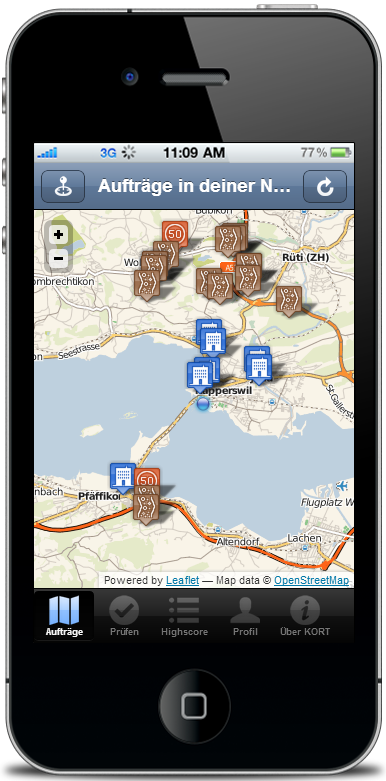
\includegraphics[width=0.3\textwidth]{images/screenshots/kort-screenshot-bugmap}}
\hfill
\subfigure{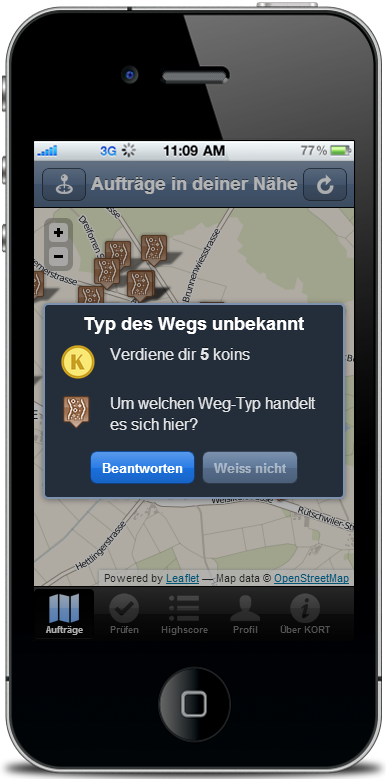
\includegraphics[width=0.3\textwidth]{images/screenshots/kort-screenshot-bugmap_message_box}}
\hfill
\subfigure{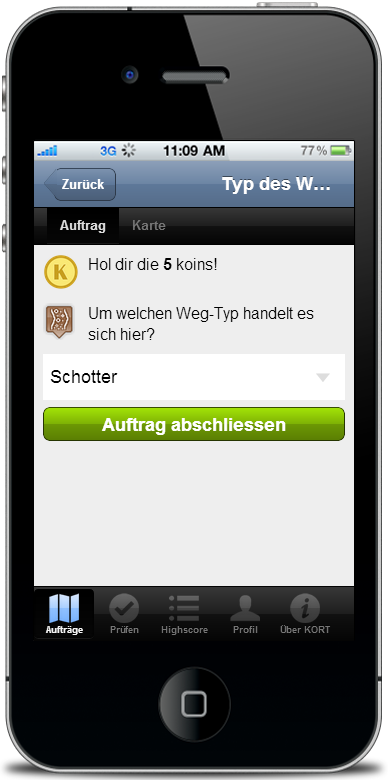
\includegraphics[width=0.3\textwidth]{images/screenshots/kort-screenshot-fix}}
\caption{Maske: Aufträge}
\label{maske-auftraege}
\end{figure}

\subsection{Maske: Prüfen}
In der \emph{Prüfen}-Maske werden dem Benutzer die Lösungen angezeigt, welche noch zu überprüfen sind (siehe Abbildung \ref{maske-pruefen}).
Diese sind dabei nach der Anzahl noch nötiger Überprüfungen gruppiert.
So soll erreicht werden, dass Lösungen, die schon bald an \brand{OpenStreetMap} zurückgesendet werden können, bevorzugt behandelt werden.
In der Liste werden maximal 25 Überprüfungen angezeigt.

Sobald der Benutzer einen Eintrag auswählt, wird ihm neben der eingetragenen Lösung auch der Fehler auf der Karte angezeigt.
Er kann nun beurteilen, ob diese Lösung korrekt oder falsch ist.

\begin{figure}[H]
\subfigure{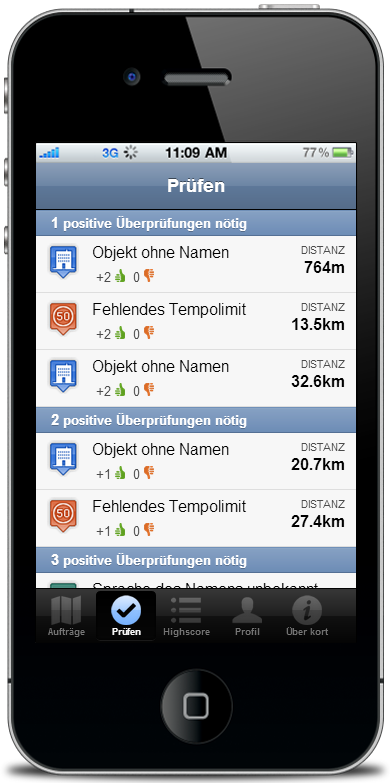
\includegraphics[width=0.3\textwidth]{images/screenshots/kort-screenshot-validation}}
\hfill
\subfigure{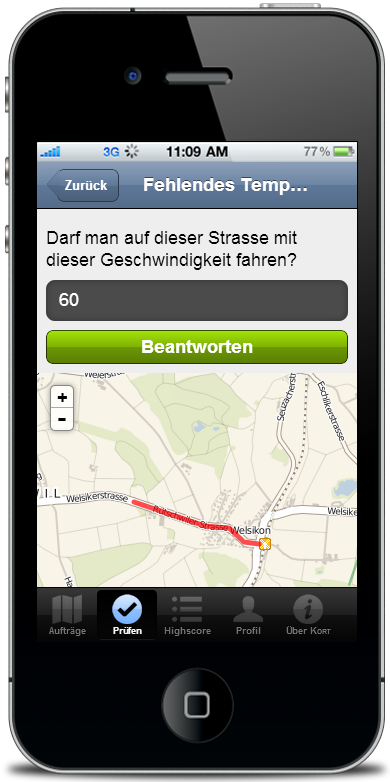
\includegraphics[width=0.3\textwidth]{images/screenshots/kort-screenshot-vote}}
\hfill
\subfigure{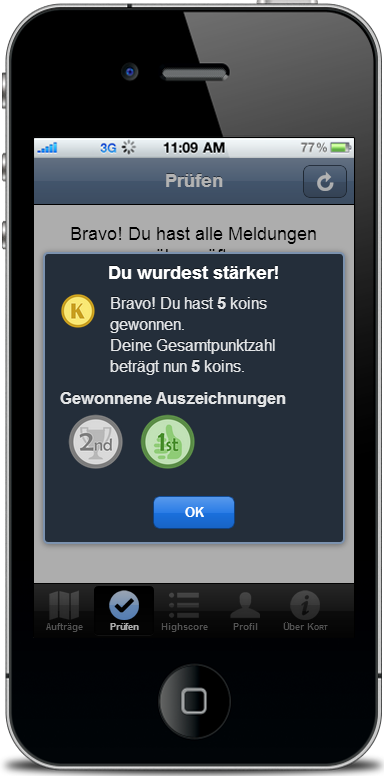
\includegraphics[width=0.3\textwidth]{images/screenshots/kort-screenshot-reward}}
\caption{Maske: Prüfen}
\label{maske-pruefen}
\end{figure}

\subsection{Maske: Highscore}
In der Highscore werden die Benutzer nach Anzahl gewonnener Punkte (sog. \emph{Koins}) sortiert (siehe Abbildung \ref{masken-highscore-profile-about}).
Es werden jeweils die ersten zehn Platzierungen angezeigt.

Wird ein Eintrag in der Highscore-Liste ausgewählt, so kann man sich das Profil des jeweiligen Benutzers anschauen.

\subsection{Maske: Profil}
Im Profil findet man eine Zusammenfassung seiner persönlichen Spielaktivitäten.
Man sieht die Gesamtanzahl der gesammelten \emph{Koins} und eine Übersicht der gewonnen Auszeichnungen (siehe Abbildung \ref{masken-highscore-profile-about}).

Auf der Profilseite lassen sich die Auszeichnungen auch in Grossformat anzeigen.

\subsection{Maske: Über Kort}
Auf der \emph{Über Kort}-Seite werden allgemeine Informationen zur Applikation angezeigt (siehe Abbildung \ref{masken-highscore-profile-about}).

\begin{figure}[H]
\subfigure{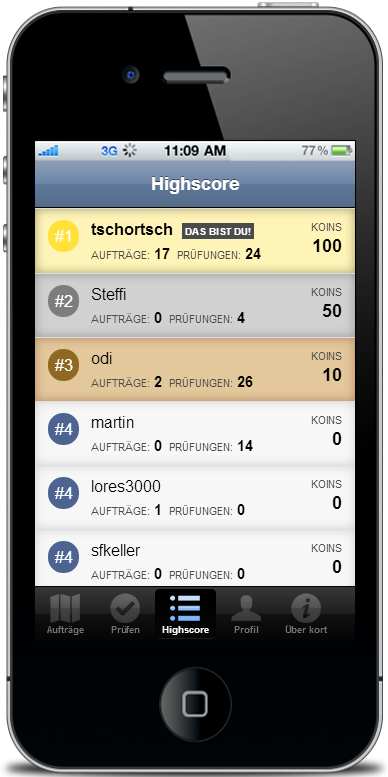
\includegraphics[width=0.3\textwidth]{images/screenshots/kort-screenshot-highscore}}
\hfill
\subfigure{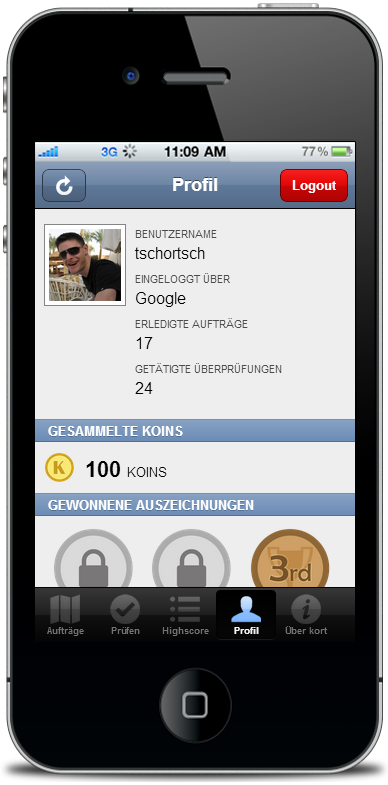
\includegraphics[width=0.3\textwidth]{images/screenshots/kort-screenshot-profile}}
\hfill
\subfigure{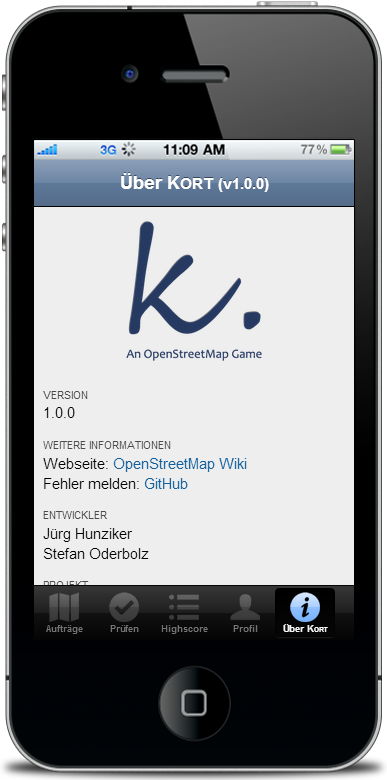
\includegraphics[width=0.3\textwidth]{images/screenshots/kort-screenshot-about}}
\caption{Masken: Highscore / Profil / Über \kort{}}
\label{masken-highscore-profile-about}
\end{figure}

% Dokumentation
% Dokumentation
\section{Dokumentation}

Das Frontend von \kort{} ist durchgängig mit der Sencha-eigenen Dokumentationssprache \brand{JSDuck}\footnote{\url{https://github.com/senchalabs/jsduck}} dokumentiert.
Die Dokumentation findet sich unter: \url{http://kort.herokuapp.com/docs/Kort}.

\begin{figure}[H]
	\centering
	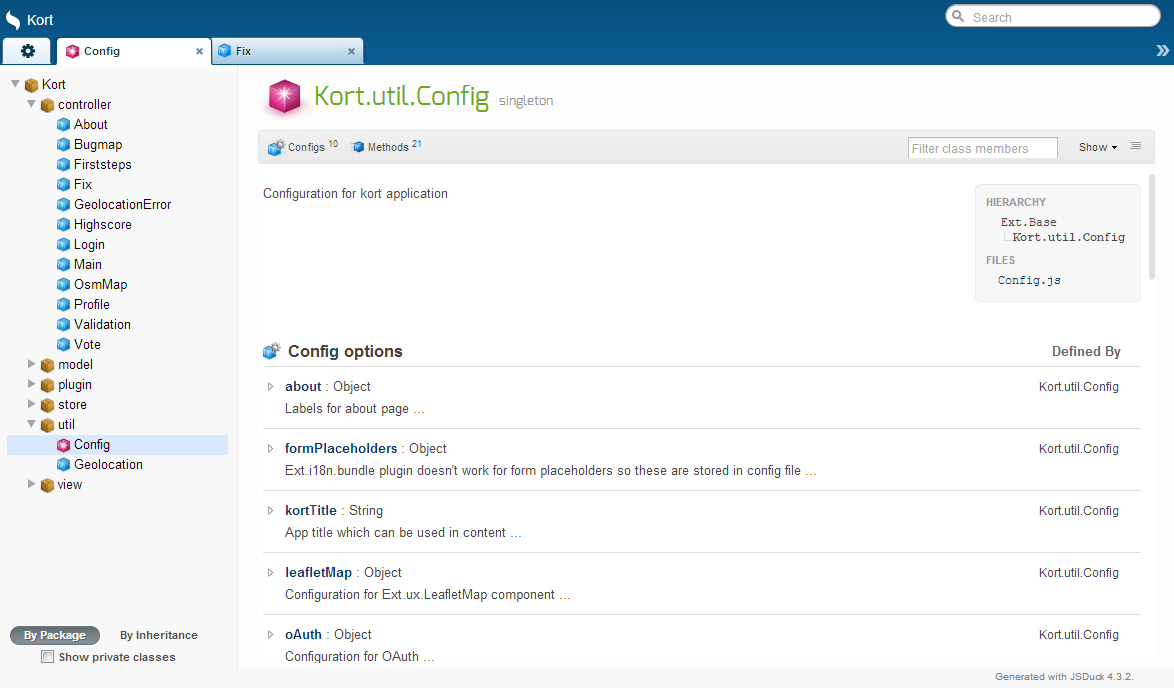
\includegraphics[scale=0.33]{images/implementation/frontend/kort-documentation}
	\caption{Frontend Dokumentation mit JSDuck}
	\label{image-kort-documentation}
\end{figure}

% Bekannte Fehler
% Bekannte Fehler
\section{Bekannte Fehler}

\subsection{iOS6 - Add to homescreen}
Eine sehr nützliche Funktionalität, welche Apple im Mobile Safari-Browser anbietet ist die \emph{Add to homescreen}-Funktion.

\begin{figure}[H]
\subfigure{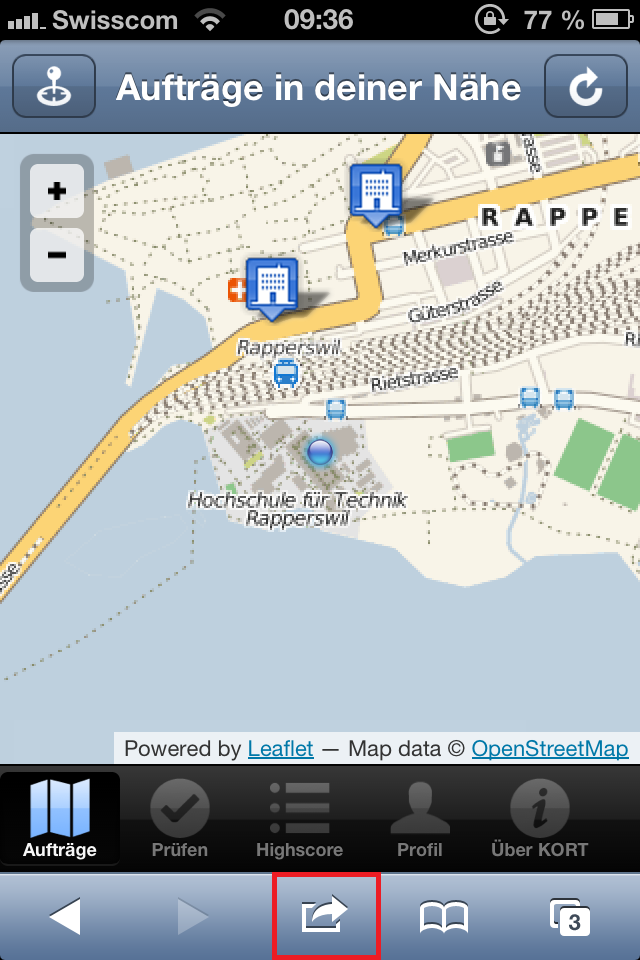
\includegraphics[width=0.23\textwidth]{images/bugs/kort-add_to_homescreen_1}}
\hfill
\subfigure{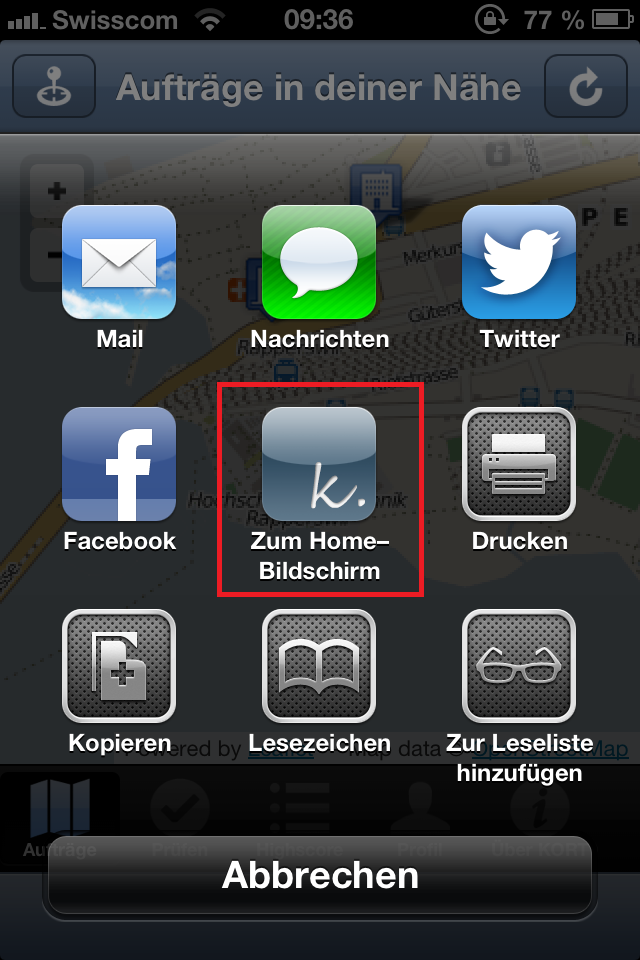
\includegraphics[width=0.23\textwidth]{images/bugs/kort-add_to_homescreen_2}}
\hfill
\subfigure{
\includegraphics[width=0.23\textwidth]{images/bugs/kort-add_to_homescreen_3}}
\hfill
\subfigure{
\includegraphics[width=0.23\textwidth]{images/bugs/kort-add_to_homescreen_4}}
\caption{iOS Add to homescreen-Funktion}
\end{figure}

Dadurch wird ein App-ähnliches Bookmark der aktuellen Webseite auf dem Homescreen erstellt.
Dieser erhält ein hinterlegtes Icon und einen Titel.
Beim Starten der App erscheint ein Splashscreen, welchen man ebenfalls in der Webseite definieren kann.
Zudem öffnet sich der Browser ohne jegliche Toolbars wie  Adress- oder Navigationsleiste.

Leider befindet sich in iOS6 ein Bug, welcher den Zugriff auf die Geolocation verhindert, wenn die \gls{WebApp} vom Homescreen aus gestartet wird.
Auf StackOverflow\footnote{\url{http://stackoverflow.com/questions/12503815/ios-6-breaks-geolocation-in-webapps-apple-mobile-web-app-capable}} wird der Bug genauer beschrieben.

\subsubsection{Workaround}
Im Sencha Forum\footnote{\url{http://www.sencha.com/forum/showthread.php?246317-2.1.0-RC1-Save-to-home-screen-Geolocation-not-working}} wird als Workaround vorgeschlagen, die Generierung des \newline \inlinecode{apple-mobile-web-app-capable} Metatags in der Sencha Touch Library zu deaktivieren (siehe Code-Ausschnitte \ref{code-ios6-homescreen-metatag} und \ref{code-ios6-bug-workaround}).

\lstset{language=HTML}
\begin{lstlisting}[caption=Metatag{,} welcher iOS6 Bug hervorruft, label=code-ios6-homescreen-metatag]
<meta content="yes" name="apple-mobile-web-app-capable" />
\end{lstlisting}

\lstset{language=JavaScript}
\begin{lstlisting}[caption=iOS6 Bug Workaround, label=code-ios6-bug-workaround]
//meta('apple-mobile-web-app-capable', 'yes');
\end{lstlisting}

Das Deaktivieren dieser Zeile hat aber zur Folge, dass der native Rahmen des Browsers (Adressleiste, Navigationsleiste) wieder angezeigt wird.
Dies ist zwar unschön, löst aber das Problem mit dem Zugriff auf die Geolocation.

\subsection{App Build}
Wie in Abschnitt \ref{sencha-cmd} beschrieben, basiert die App vollständig auf dem Sencha-eigenen Build-Tool \brand{Sencha Cmd}. Darin sind aber noch einige Bugs vorhanden.

Bei \kort{} besteht dabei ein Problem bei der fest eingebauten Komprimierung der JavaScript-Sourcen.
Während diesem Prozess werden lokale Variablennamen mit einzelnen Buchstaben abgekürzt, um die Dateigrösse zu reduzieren.
Dabei treten Konflikte mit der \brand{Leaflet}-Library auf, welche den Buchstaben \emph{L} als Namespace verwendet.

\subsubsection{Workaround}
Um diese Problem zu umgehen, mussten wir das Build-Skript von \brand{Sencha Cmd} minimal anpassen.
So mussten wir die Zeile, welche den \gls{Microloader} komprimiert, auskommentieren (siehe Code-Ausschnitt \ref{senchacmd-workaround}).
Diese befindet sich in folgender Datei:

\inlinecode{/<Sencha Cmd Verzeichnis>/plugins/touch/current/app-build.js} Zeile 362

\lstset{language=JavaScript}
\begin{lstlisting}[caption=Sencha Cmd Workaround, label=senchacmd-workaround]
processIndex = function () {
	[...]
	compressor = new ClosureCompressor();
	microloader = (environment == 'production'
		? 'production'
		: 'testing') +
		'.js';
	_logger.debug("using microloader : {}", microloader);
	content = readFileContent(joinPath(sdk, "microloader", microloader));
	//content = compressor.compress(content);
	remotes = [
		'<script type="text/javascript">' +
			content + ';Ext.blink(' +
			(environment == 'production' ? jsonEncode({
				id:config.id
			}) : appJson) + ')' +
			'</script>'
	];
	[...]
};
\end{lstlisting}

% Leaflet Sencha Touch Komponente
\chapter{OpenStreetMap-Daten in Sencha Touch}
\label{leaflet-sencha-komponente}

\section{Sencha Touch Map-Komponente}

Das Sencha Touch 2-Framework bietet zur Darstellung einer Karte lediglich eine Google Maps-Komponente an.
Diese ist stark auf das Google Maps API ausgerichtet und kann deshalb nicht für andere Kartendaten verwendet werden.

Um trotzdem Daten von \brand{OpenStreetMap} verwenden zu können, mussten wir eine neue Sencha Touch Map-Komponente erstellen, welche eine für diesen Zweck vorgesehene Library verwendet.

\section{Leaflet Map-Komponente}

Zur Darstellung der OSM-Daten verwendeten wir zuerst die \brand{OpenLayers}\footnote{\url{http://openlayers.org/}}-Library.
Leider mussten wir nach einiger Zeit feststellen, dass diese für unsere Zwecke zu komplex und überladen ist.

Wir haben deshalb eine Komponente erstellt, welche die \brand{Leaflet}\footnote{\url{http://leafletjs.com/}}-Library zur Darstellung der Karte verwendet.
Leaflet ist eine moderne, leichtgewichtige Karten-Library.
Sie wurde speziell für den Einsatz auf mobilen Geräten konzipiert.
Zusätzlich ist sie sehr gut dokumentiert und lässt sich einfach bedienen.

\begin{figure}[H]
	\centering
	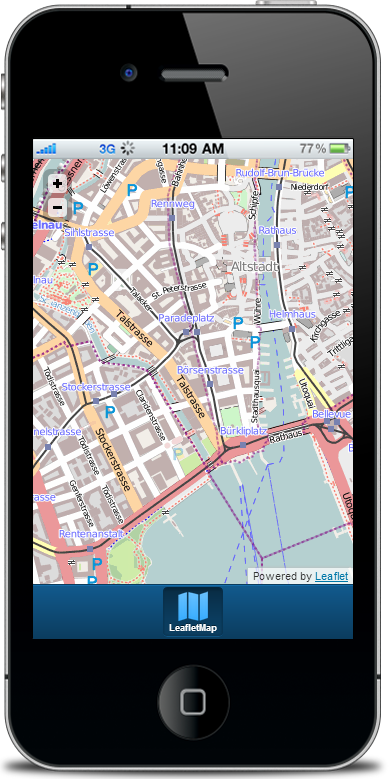
\includegraphics[scale=0.5]{images/implementation/frontend/leafletmap-screenshot}
	\caption{Ext.ux.LeafletMap-Komponente in Sencha Touch}
	\label{image-leafletmap-screenshot}
\end{figure}

\subsection{Verfügbarkeit}
Unsere Sencha Touch Komponente war zuletzt so ausgereift, dass wir uns entschieden haben, diese für die Allgemeinheit zugänglich zu machen.
Wir veröffentlichten sie deshalb unter dem Namen \brand{Ext.ux.LeafletMap} im offiziellen Sencha Market\footnote{\url{http://market.sencha.com/}}.
Sie ist verfügbar unter: \url{https://market.sencha.com/users/162/extensions/177}.

\begin{table}[H]
\centering
\begin{tabular}{|p{0.2\twocelltabwidth}|p{0.8\twocelltabwidth}|}
\hline 
\textbf{Ort} & \textbf{URL} \\ 
\hline 
Sencha Market & \url{https://market.sencha.com/users/162/extensions/177} \\ 
\hline 
GitHub & \url{https://github.com/tschortsch/Ext.ux.LeafletMap} \\ 
\hline 
\end{tabular} 
\caption{Ext.ux.LeafletMap Verfügbarkeit}
\label{leafletmap-availiblity}
\end{table}

\begin{figure}[H]
	\centering
	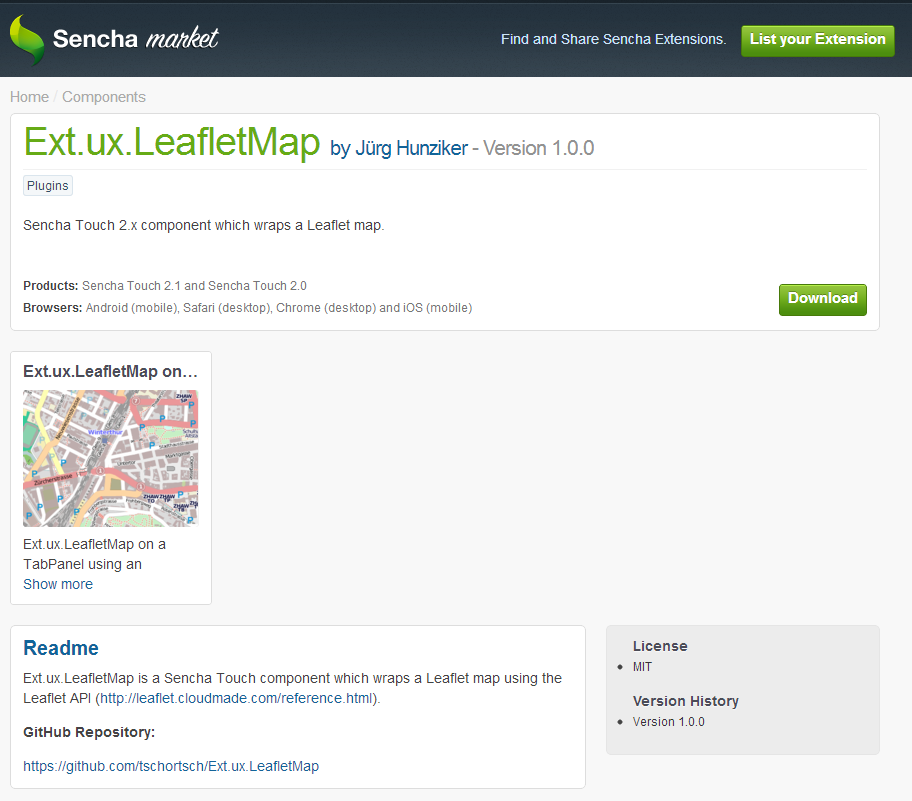
\includegraphics[scale=0.6]{images/implementation/frontend/leafletmap-sencha-market}
	\caption{Leaflet Map-Komponente im Sencha Market}
	\label{image-leafletmap-sencha-market}
\end{figure}

\subsection{Dokumentation}
Die Komponente ist durchgängig mit der Sencha-eigenen JavaScript-Dokumentationssprache \brand{JSDuck}\footnote{\url{https://github.com/senchalabs/jsduck}} dokumentiert. Die Dokumentation befindet sich unter: \url{http://kort.herokuapp.com/docs/Ext.ux.LeafletMap}.

% Gamification
\chapter{Gamification}
\label{gamification}

Unter \gls{Gamification} versteht man die Verwendung von spieltypischen Elementen in einem spielfremden Kontext.
Die bekanntesten Elemente dabei sind die Punktevergabe für das Lösen von Aufgaben, die Verleihung von Badges für besonders engagierte Einsätze oder das Bereitstellen einer Highscore zum Vergleich mit anderen Benutzern.

Während unserer Arbeit hatten wir verschiedene Partner, welche uns bei der \gls{Gamification} unserer Applikation unterstützen.
So ist unserer Industriepartner Reto Senn Mitinhaber der Firma bitforge AG\footnote{\url{http://bitforge.ch/}}, welche sich auf Games im mobilen Umfeld spezialisiert hat.
Er konnte uns vor und während der Entwicklung viele wertvolle Tipps zur Verbesserung des Spielgefühls geben.

\section{Gamification in Kort}
\subsection{Sprache}
\gls{Gamification} findet sich nicht nur in schönen Grafiken und Spiel-Elementen.
Sie beginnt bereits bei der Sprachwahl von Texten.
Beim Lesen der Texte sollte eine gewisse Spannung aufgebaut werden.
Dadurch erhöht sich die Motivation, die anstehende Aktion durchzuführen.

In \kort{} findet sich dafür ein Beispiel in der Button-Bezeichnung bei der Eingabe des eigenen Benutzernamens.
Zu Beginn war dieser mit "`App starten"' beschriftet.
Wir haben ihn aber später mit dem Text "`Mission beginnen!"' ersetzt.
Weiter wurde der Button grün eingefärbt, um ihn zusätzlich vom Text und vom Hintergrund abzuheben.

\begin{figure}[H]
	\centering
	
\includegraphics{images/gamification/gamification-lang-firststeps}
	\caption{Gamification - Sprache}
	\label{gamification-lang-firststeps}
\end{figure}

Neben der gewählten Ausdrucksweise sollte die Sprache dem Zielpublikum angepasst werden.
Wir mussten dafür viele Begriffe aus dem \glslink{Mapper}{Mapping}-Vokabular für unsere breite Zielgruppe mit allgemeineren Wörtern ersetzen.

\subsection{Punktesystem "`Koins"'}
Eines der wichtigsten Elemente im Spiel bildet das Punktesystem. Dieses findet sich in beinahe allen Aktionen der App wieder.
So gewinnt ein Spieler für gelöste Aufgaben oder getätigte Prüfungen eine gewisse Anzahl an sogenannten \emph{Koins}.
Mit der Anzahl \emph{Koins} kann er sich wiederum in der Highscore mit den anderen Spieler messen.

\begin{figure}[H]
	\centering
	
\includegraphics[scale=0.4]{images/gamification/gamification-koin}
	\caption{Gamification - Koins}
	\label{gamification-koins}
\end{figure}

\subsection{Auszeichnungen}
Zusätzlich zu den \emph{Koins} kann ein Spieler Auszeichnungen gewinnen. Diese erhält er durch besondere Leistungen. In \kort{} sind momentan folgende Auszeichnungen implementiert:

\begin{table}[H]
\centering
\begin{tabular}{|p{0.25\twocelltabwidth}|p{0.75\twocelltabwidth}|}
\hline 
\textbf{Auszeichnungstyp} & \textbf{Beschreibung} \\ 
\hline 
Anfänger & Eine Auszeichnungen für das Lösen des 1. Auftrags und eine für das Überprüfen der 1. Antwort. \\ 
\hline 
Platzierung & Drei Auszeichnungen für das Erreichen des 1., 2. und 3. Rangs in der Highscore. \\ 
\hline 
Aufträge & Drei Auszeichnungen für das Lösen von 10, 50 und 100 Auträgen. \\ 
\hline 
Prüfungen & Drei Auszeichnungen für 10, 10 und 1000 geprüfte Antworten. \\ 
\hline 
\end{tabular} 
\caption{Auszeichnungen in \kort{}}
\label{kort-badges}
\end{table}

\begin{figure}[H]
	\centering
	
\includegraphics[scale=0.7]{images/gamification/gamification-badges}
	\caption{Gamification - Badges}
	\label{gamification-badges}
\end{figure}

Das Hinzufügen von zusätzlichen Auszeichnungen wird in Abschnitt \ref{kort-additional-badges} beschrieben.

\subsection{Highscore}
Über die Highscore haben die Benutzer der App die Möglichkeit sich mit den anderen Spielern zu vergleichen.
Dazu werden sie nach Anzahl gewonnener \emph{Koins} in einer Rangliste eingestuft.

\section{Weitere mögliche Elemente}
Neben den verwendeten \gls{Gamification}-Elementen in \kort{} gibt es noch eine Vielzahl weiterer Elemente, welche sich für diesen Anwendungszweck eignen würden.
Diese konnten während der Arbeit aber nicht implementiert werden.

Daneben gibt es aber auch noch Elemente, welche zwar für \brand{OpenStreetMap} als Projekt interessant wären, sich jedoch nicht mit \kort{} umsetzen lassen.

Diese werden in der Folge genauer beschrieben.

\subsection{Erste Schritte}
Um den Einstieg in die Verwendung der App weiter zu vereinfachen, wäre es sinnvoll, beim ersten Start eine kurze Einführung anzuzeigen.
So könnte man dem Benutzer für die einzelnen Masken jeweils Tipps einblenden oder gar eine geführte Tour durch die App und deren Möglichkeiten anbieten.

Wenn der Benutzer nicht weiss, welche Möglichkeiten er hat, kann dies dazu führen, dass er schnell wieder aufgibt oder nicht das volle Potential der App ausschöpfen kann.

\subsection{Zeitlich begrenze Aktionen}
Durch das Einführen von zeitlich begrenzten Aktionen kann man Benutzer dazu motivieren, die App über einen längeren Zeitraum zu verwenden.
So könnte man Tage definieren, an denen man die doppelte Anzahl an Punkten gewinnt.
Zusätzlich könnte man Aktionen\footnote{Beispiel einer zeitlich begrenzen Aktion in \brand{OpenStreetMap}: Das \brand{big baseball project 2011} \url{http://wiki.openstreetmap.org/wiki/Big_baseball_project_2011}} starten, bei denen man spezielle Auszeichnungen gewinnen kann.

Um den Benutzer dazu zu animieren, die App erneut zu starten, könnte man per Push-Meldungen auf aktuelle Aktionen, Updates oder Ereignisse aufmerksam machen.

\subsection{Weitere Auszeichnungen hinzufügen}
Bei der Auswahl an verfügbaren Auszeichnungen sollte man darauf achten, dass es für jeden Spielertyp geeignete Auszeichnungen zu gewinnen gibt.
Die verschiedenen Typen haben eine ganz andere Herangehensweise und müssen deshalb auch mit verschiedenen Belohnungen motiviert werden.
Eine Einteilung von verschiedenen Spielertypen wird auf \brand{Gamasutra}\footnote{\url{http://www.gamasutra.com/view/feature/6474/personality_and_play_styles_a_.php}} beschrieben.

Es gibt bereits eine Liste von möglichen Badges im Wiki von OpenStreetMap\footnote{\url{https://wiki.openstreetmap.org/wiki/Badges}}.

\subsection{Verschiedene Highscores}
Durch das Bereitstellen von verschiedenen Highscores (Bsp. Regional, Nach Fehlertyp), gibt man allen Benutzern die Chance, irgendwo den ersten Platz zu erreichen.
Dadurch verhindert man eine mögliche Demotivation beim Vergleich mit Langzeitspielern, welche bereits eine grosse Anzahl an Punkten gesammelt haben.

\subsection{Erfahrene Spieler}
Man könnte als Belohnung für viele gelöste Fehler die Berechtigungen des Benutzers erhöhen.
So könnte beispielsweise seine Stimme bei einer Überprüfung einer Lösung doppelt zählen.
Dieses Prinzip wird auch von der Frage/Antwort-Plattform \brand{StackOverflow}\footnote{\url{http://stackoverflow.com/}} angewendet.

\begin{figure}[H]
	\centering
	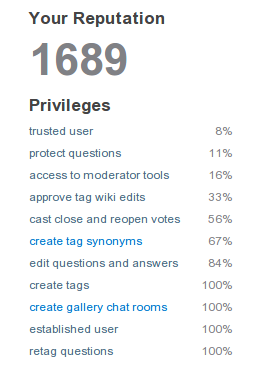
\includegraphics[scale=0.7]{images/gamification/so-privileges}
	\caption{Zusätzliche Berechtigungen bei StackOverflow}
	\label{gamification-so-privileges}
\end{figure}

Um einen erfahrenen Spieler nicht zu unterfordern, könnte man ihm beim Erreichen einer gewissen Punktzahl, Fehler anzeigen, welche schwieriger zu lösen sind.
Wichtig ist es dabei, dass das Spiel nicht plötzlich vorbei ist.
Auch der Spieler, der bereits die meisten Punkte hat, muss noch eine Motivation haben, die App weiter zu verwenden.

\subsection{Einbinden in Apple Game Center}
Apple bietet mit dem \brand{Game Center} einen zentralen Ort an, Punkte und Auszeichnungen von Game-Apps zu speichern.
Dadurch können sich Spieler direkt mit anderen Spielern und Kollegen, die ebenfalls diese App verwenden, vergleichen.
Dadurch, dass das \brand{Game Center} bereits eine grosse Community an Spielern aufweist, wäre es von Vorteil, die App darin einzubinden.
Leider besteht dabei die Einschränkung, dass man lediglich iOS-Games für das Game Center anmelden kann.

\begin{figure}[H]
	\centering
	
\includegraphics{images/gamification/apple-game-center}
	\caption{Apple Game Center}
	\label{image-gamification-apple-game-center}
\end{figure}

\subsection{Design}
Spiele habe viele Design-Eigenheiten, welche sich von reinen Business-Applikationen abheben.
Dies kann durch geeignete Farben und UI-Elemente realisiert werden.
Typischerweise wird ein Benutzer durch die Applikation geführt, so dass ihm immer klar ist, wie es weiter geht.

\subsection{Gamification von OpenStreetMap}
In der \brand{OpenStreetMap} Community gibt es bereits einige Ideen um Spiele-Konzepte für das Projekt zu verwenden\footnote{z.B. von Prof. Stefan Keller initiierte Diskussion auf der Geowanking-Mailingliste: \url{http://geowanking.org/pipermail/geowanking_geowanking.org/2012-September/thread.html\#26302}}.

An der State Of The Map Konferenz 2011 (SotM 2011) hat Martijn van Exel  einen Vortrag zum Thema \emph{Can gaming concepts help make OpenStreetMap better?}\footnote{\url{http://wiki.openstreetmap.org/wiki/SotM_2011_session:_Insert_Coin_To_Play}} gehalten.
Er beschreibt darin eines der Hauptprobleme von \brand{OpenStreetMap}, dass es neuen Benutzern schwerfällt die \emph{erste Meile} zurückzulegen.
Viele neue Benutzer haben Angst davor etwas falsch zu machen und müssen sich zuerst mit den vielfältigen Möglichkeiten des Karten-Editors vertraut machen.
Die Statistik der Benutzer von \brand{OpenStreetMap} bestätigt dieses Bild: fast zwei Drittel der Benutzer hat noch nie Änderungen vorgenommen\footnote{\url{http://osmstats.altogetherlost.com/}}.

Martijn van Exel schlägt deshalb vor, dass das Recht die Karte zu editieren gestaffelt werden soll.
So soll sich ein Benutzer das Recht "`verdienen"' müssen, komplexere Änderungen an der Karte vorzunehmen.

Dadurch kann der Spieltrieb des Menschen geweckt werden, um sich weiterzuentwickeln.
Nebenbei lernt der Benutzer den Umgang mit dem Karteneditor und fühlt sich zunehmend sicherer überhaupt Änderungen vorzunehmen.

% Datenquellen
\chapter{Fehler-Datenquellen}
\label{datenquellen}
Die Grundlage unserer \gls{WebApp} bilden die Fehlerdaten, welche korrigiert werden sollen.
Deshalb musste zuerst eine geeignete Quelle für Fehlerdaten von \brand{OpenStreetMap} gefunden werden.

\section{Evaluation von geeigneten Datenquellen}
Durch die Anforderungen an die Applikation ergaben sich folgende Bedingungen, welche die Fehlerdaten erfüllen müssen:

\begin{itemize}
\item Die Fehler müssen auch für Nicht-\gls{Mapper} lösbar sein.
\item Sie müssen auf Deutsch übersetzbar sein. Die Fehlerbeschreibungen sollten somit einem gegebenen Schema folgen und keinen Freitext beinhalten.
\item Die Fehler müssen sich einfach in einem UI abbilden lassen.
\item Die Fehler sollen sich nur auf Metadaten beziehen und nicht auf Geometrieobjekte (Strasse, Gebäude, usw.), da wir keinen vollwertigen Karten-Editor anbieten können.
\item Die Fehler sollen sich immer nur auf einen \gls{Tag} des betroffenen \brand{OpenStreetMap}-Objekts beziehen. Dadurch vereinfacht sich das Zurückschreiben der Daten zu \brand{OpenStreetMap}.
\end{itemize}

Wir untersuchten mehrere mögliche Fehlerdatenquellen im Hinblick auf ihre Qualität.

\subsection{Fehler aus OpenStreetMap extrahieren}
Da die Daten von \brand{OpenStreetMap} frei verfügbar sind, steht es jedem offen, diese Daten zu nutzen und selbst zu verarbeiten.
Es wäre somit eine Möglichkeit, sich selbst daran zu versuchen, Fehler mit geeigneten Regeln zu finden und aus den Daten zu extrahieren.

\begin{table}[H]
\centering
\begin{tabular}{|p{0.3\twocelltabwidth}|p{0.7\twocelltabwidth}|}
\hline 
\small{\textbf{URL}} & \url{http://www.openstreetmap.org} \\
\hline 
\small{\textbf{Erfasser}} & Backend von \kort{} \\
\hline 
\small{\textbf{API verfügbar?}} & Ja (\gls{REST} \gls{API}) \newline
\url{http://wiki.openstreetmap.org/wiki/API_v0.6} \\
\hline 
\small{\textbf{Lösung zurückschreiben}} & Lösung könnte via \gls{API} an \brand{OpenStreetMap} gesendet werden. \\
\hline
\small{\textbf{Eignung}} & \textbf{schlecht} \linebreak Das Finden von Fehlern ist komplex, da es sehr viele Ausnahmen zu beachten gibt.
Dies würde den Rahmen dieser Arbeit sprengen. \\ 
\hline 
\end{tabular} 
\caption{Fehler aus OpenStreetMap}
\label{datenquellen-osm_itself}
\end{table}

\subsection{FIXME-Tags in OpenStreetMap}
Fehlerhafte Objekte in \brand{OpenStreetMap} können von Benutzern direkt mit einem \inlinecode{FIXME}-\gls{Tag} versehen werden, wenn sie einen Fehler aufweisen.
Darin wird der eigentliche Fehler beschrieben.

\begin{table}[H]
\centering
\begin{tabular}{|p{0.3\twocelltabwidth}|p{0.7\twocelltabwidth}|}
\hline 
\small{\textbf{URL}} & \url{http://wiki.openstreetmap.org/wiki/DE:Key:fixme} \\
\hline 
\small{\textbf{Erfasser}} & \brand{OpenStreetMap}-Benutzer \\
\hline 
\small{\textbf{API verfügbar?}} & Ja (\gls{REST} \gls{API}) \newline
\url{http://wiki.openstreetmap.org/wiki/API_v0.6} \\
\hline 
\small{\textbf{Lösung zurückschreiben}} & Lösung könnte via \gls{API} an \brand{OpenStreetMap} gesendet werden. \\
\hline
\small{\textbf{Eignung}} & \textbf{schlecht} \linebreak Durch die manuelle Erfassung der Daten, ist es für uns nicht möglich, automatisiert ein GUI für die Fehlerbehebung zu erstellen. \\ 
\hline 
\end{tabular} 
\caption{FIXME-Tags in OpenStreetMap}
\label{datenquellen-fixme_tags_osm}
\end{table}

\subsection{OpenStreetBugs}
\label{openstreetbugs}
Mit der Applikation \brand{OpenStreetBugs} ist es für die Benutzer möglich, Fehler in den Kartendaten als Bug zu erfassen.

\begin{table}[H]
\centering
\begin{tabular}{|p{0.3\twocelltabwidth}|p{0.7\twocelltabwidth}|}
\hline 
\small{\textbf{URL}} & \url{http://openstreetbugs.schokokeks.org/} \\
\hline 
\small{\textbf{Erfasser}} & OpenStreetBugs-Benutzer \\
\hline 
\small{\textbf{API verfügbar?}} & Ja (\gls{REST} \gls{API} oder Fehlerdaten als Dump-File downloadbar) \newline
\url{http://wiki.openstreetmap.org/wiki/OpenStreetBugs/API_0.6} \\
\hline 
\small{\textbf{Lösung zurückschreiben}} & Lösung müsste an \brand{OpenStreetMap} gesendet werden. Zusätzlich  müsste der Bug auf OpenStreetBugs als gelöst markiert werden. \\
\hline
\small{\textbf{Eignung}} & \textbf{schlecht} \linebreak Die erfassten Daten sind Freitext. Sie eigenen sich daher nicht für die automatisierte Erstellung eines GUIs. \\ 
\hline 
\end{tabular} 
\caption{OpenStreetBugs}
\label{datenquellen-openstreetbugs}
\end{table}

\subsection{KeepRight}
\brand{KeepRight} ist ein Dienst, welcher jeweils über Nacht Fehler in OSM-Objekten sucht und in einer eigenen Datenbank ablegt.

\begin{table}[H]
\centering
\begin{tabular}{|p{0.3\twocelltabwidth}|p{0.7\twocelltabwidth}|}
\hline 
\small{\textbf{URL}} & \url{http://keepright.ipax.at} \\
\hline 
\small{\textbf{Erfasser}} & Automatisiert durch nächtlichen Job \\
\hline 
\small{\textbf{API verfügbar?}} & Ja (Fehlerdaten werden als Dump-File zum Download angeboten) \newline \url{http://keepright.ipax.at/interfacing.php} \\
\hline 
\small{\textbf{Lösung zurückschreiben}} & Lösung müssten lediglich an \brand{OpenStreetMap} gesendet werden. \brand{KeepRight} baut seine Fehlerdatenbank jeweils über Nacht aus den \brand{OpenStreetMap}-Daten neu auf. \\
\hline
\small{\textbf{Eignung}} & \textbf{gut} \linebreak Dadurch, dass die Fehlerdaten automatisiert erstellt werden, ist es gut möglich, für jeweilige Fehlertypen eine geeignete Maske für deren Behebung zur Verfügung zu stellen. \\
\hline
\end{tabular}
\caption{KeepRight}
\label{datenquellen-keepright}
\end{table}

\subsection{MapDust}
\brand{MapDust} ist ein Bug-Tracker der Firma skobbler\footnote{\url{http://www.skobbler.de/}}.
Er ist \brand{OpenStreetBugs} (siehe Abschnitt \ref{openstreetbugs}) sehr ähnlich, konzentriert sich aber mehr auf Fehler beim \gls{Routing}.

\begin{table}[H]
\centering
\begin{tabular}{|p{0.3\twocelltabwidth}|p{0.7\twocelltabwidth}|}
\hline 
\small{\textbf{URL}} & \url{http://www.mapdust.com/} \\
\hline 
\small{\textbf{Erfasser}} & Benutzer von skobbler \\
\hline 
\small{\textbf{API verfügbar?}} & Ja (Dump-File der Fehler sowie \gls{API}) \newline siehe \url{http://wiki.openstreetmap.org/wiki/MapDust} \\
\hline 
\small{\textbf{Lösung zurückschreiben}} & Korrekturen können direkt an \brand{OpenStreetMap} geschickt werden.
Zusätzlich muss der Bug bei MapDust geschlossen werden. \\
\hline
\small{\textbf{Eignung}} & \textbf{mittel} \linebreak Die Qualität der Fehler lässt sehr zu wünschen übrig, da sie meist von unerfahrenen Benutzern erstellt werden. Positiv ist, dass es eine Vielzahl von Fehlern gibt und auch ein API angeboten wird. \\
\hline
\end{tabular}
\caption{MapDust}
\label{datenquellen-mapdust}
\end{table}

\subsection{Housenumbervalidator}
Der \brand{Housenumbervalidator} ist ein Quelle, welche die \brand{OpenStreetMap}-Daten automatisiert auf fehlerhafte Adressen prüft.
Die Fehler reichen von falschen Strassennamen bis zu Duplikaten von Hausnummern in der gleichen Strasse.

\begin{table}[H]
\centering
\begin{tabular}{|p{0.3\twocelltabwidth}|p{0.7\twocelltabwidth}|}
\hline 
\small{\textbf{URL}} & \url{http://gulp21.bplaced.net/osm/housenumbervalidator/} \\
\hline 
\small{\textbf{Erfasser}} & Berechnet aus \brand{OpenStreetMap} \\
\hline 
\small{\textbf{API verfügbar?}} & Nein, aber der Quellcode ist frei verfügbar. \\
\hline 
\small{\textbf{Lösung zurückschreiben}} & Korrekturen können direkt an \brand{OpenStreetMap} geschickt werden. \\
\hline
\small{\textbf{Eignung}} & \textbf{mittel} \linebreak Es ist schade, dass es kein \gls{API} des Housenumbervalidators gibt. Die Fehler sind zum Teil schwierig zu verstehen für Laien, was die Erstellung eines UIs schwierig macht. Zudem sind die Daten auf Deutschland und Österreich begrenzt. \\
\hline
\end{tabular}
\caption{Housenumbervalidator}
\label{datenquellen-housenumbervalidator}
\end{table}

\section{Entscheid: Fehlerdaten von KeepRight}
Durch die gute Eignung der Fehlerdaten vom \brand{KeepRight}-Dienst, haben wir uns dazu entschieden, deren Daten als Basis für unsere Fehler zu verwenden.
Der Dienst liefert zuverlässig Daten in hoher Qualität.
Die Fehlermeldungen sind klar und alle Fehler sind bereits kategorisiert, was es einfach macht, diese für die grafische Darstellung zu unterscheiden.

Ein grosses Plus ist auch, dass sich die Daten auf \brand{OpenStreetMap} abstützen, so dass eine Korrektur nur an einer Stelle vorgenommen werden muss.

\section{Fehlerdaten in die Datenbank laden}
Um stets aktuelle Daten für die App anzuzeigen, wird der Dump von \brand{KeepRight} jede Nacht mit einem Shellskript in die Datenbank geladen.
Das Shellskript befindet sich unter:

\inlinecode{/server/database/keepright\_setup.sh}

Mittels Cronjob wird folgender Befehl aufgerufen:

\inlinecode{\$ setup\_keepright\_db.sh -o osm -n osm\_bugs -s keepright}

\begin{table}[H]
\centering
\begin{tabular}{|p{0.25\twocelltabwidth}|p{0.75\twocelltabwidth}|}
\hline 
\small{\textbf{Parameter}} & \small{\textbf{Bedeutung}} \\
\hline 
\inlinecode{-o osm} & Datenbankbenutzer welcher das Schema besitzen soll (\emph{Owner})  \\
\hline
\inlinecode{-n osm\_bugs} & Name der Datenbank  \\
\hline
\inlinecode{-s keepright} & Name des Schemas  \\
\hline
\end{tabular}
\caption{Parameter für setup\_keepright.sh}
\label{parameter-setup-keepright}
\end{table}

\subsection{Datenformat}
Auf der Webseite von \brand{KeepRight} ist ersichtlich\footnote{\url{http://www.keepright.at/interfacing.php}}, welche Daten im Dump enthalten sind.

\begin{longtable}{|p{0.25\twocelltabwidth}|p{0.75\twocelltabwidth}|}
\hline 
\small{\textbf{Feld}} & \small{\textbf{Bedeutung}} \\
\hline 
\inlinecode{schema} & Schemabezeichner welcher die Region gemäss Planet-Karte angibt  \\
\hline
\inlinecode{error\_id} & Fehler-ID pro Schema  \\
\hline
\inlinecode{error\_type} & Typisierung des Fehlers  \\
\hline
\inlinecode{error\_name} & Name des Fehlertyps  \\
\hline
\inlinecode{object\_type} & \brand{OpenStreetMap}-Typ des Objekts (\gls{Node}, \gls{Way} oder \gls{Relation})  \\ 
\hline
\inlinecode{object\_id} & \brand{OpenStreetMap}-ID des Objekts  \\
\hline
\inlinecode{state} & Status des Fehlers (new, reopened, ignore\_temporarily, ignore)  \\
\hline
\inlinecode{msgid} & Fehlermeldung mit Platzhaltern (\$1 - \$5)  \\
\hline
\inlinecode{txt1}\newline
\inlinecode{txt2}\newline
\inlinecode{txt3}\newline
\inlinecode{txt4}\newline
\inlinecode{txt5} & Texte für Platzhalter in msgid  \\
\hline
\inlinecode{first\_occurrence} & Zeitpunkt, an dem dieser Fehler das \emph{erste} Mal entdeckt wurde \\
\hline
\inlinecode{last\_checked} & Zeitpunkt, an dem dieser Fehler das \emph{letzte} Mal entdeckt wurde \\
\hline
\inlinecode{object\_timestamp} & Letzter Änderungzeitpunkt am Objekt  \\
\hline
\inlinecode{user\_name} & Benutzer, welcher das Objekt zuletzt verändert hat  \\
\hline
\inlinecode{lat}\newline
\inlinecode{lon} & Längen- und Breitengrad des Fehlers  \\
\hline
\inlinecode{comment} & Kommentar zum Fehler  \\
\hline
\inlinecode{comment\_timestamp} & Zeitpunkt des Kommentars zum Fehler  \\
\hline
\caption{Datenformat der KeepRight-Daten}
\label{keepright-daten}
\end{longtable}

Diese Daten sind in der Tabelle \inlinecode{keepright.errors} enthalten.
Ein Subset davon wird für die Applikation benötigt.

\subsection{Internationalisierung}
\label{datenquellen-internationalisierung}
Eine Anforderung an \kort{} war es, ein deutsches UI anzubieten und daneben die App so weit vorzubereiten, dass sich diese internationalisieren lässt.
Dies schliesst selbstverständlich die Texte aus der Datenbank ein.
Alle Fehlerdaten werden ohne Übersetzung aus der Datenbank gelesen und anschliessend mit den Werten aus den Datenbank-spezifischen Properties-Files, versehen.
Die Dateien befinden sich im Verzeichnis \inlinecode{resources/i18n/}.

% Architektur
\chapter{Architektur}
\label{architektur}

Das Gesamtsystem setzt sich aus insgesamt vier Komponenten zusammen: der Datenbank, dem Webserver, der Fehlerquelle und dem Zielsystem von \brand{OpenStreetMap}. 
Die einzelnen Komponenten sind über \gls{REST}-Schnittstellen miteinander verbunden. 
Dabei sind das Zielsystem (\brand{OpenStreetMap}) und die Fehlerquelle (\brand{KeepRight}, siehe Kapitel \ref{datenquellen}) Fremdsysteme, bei welchen die Schnittstellen gegeben waren. 
Unsere eigenen Server haben wir entsprechend angepasst und auch via \gls{REST} zugänglich gemacht.

\begin{figure}[H]
	\centering
	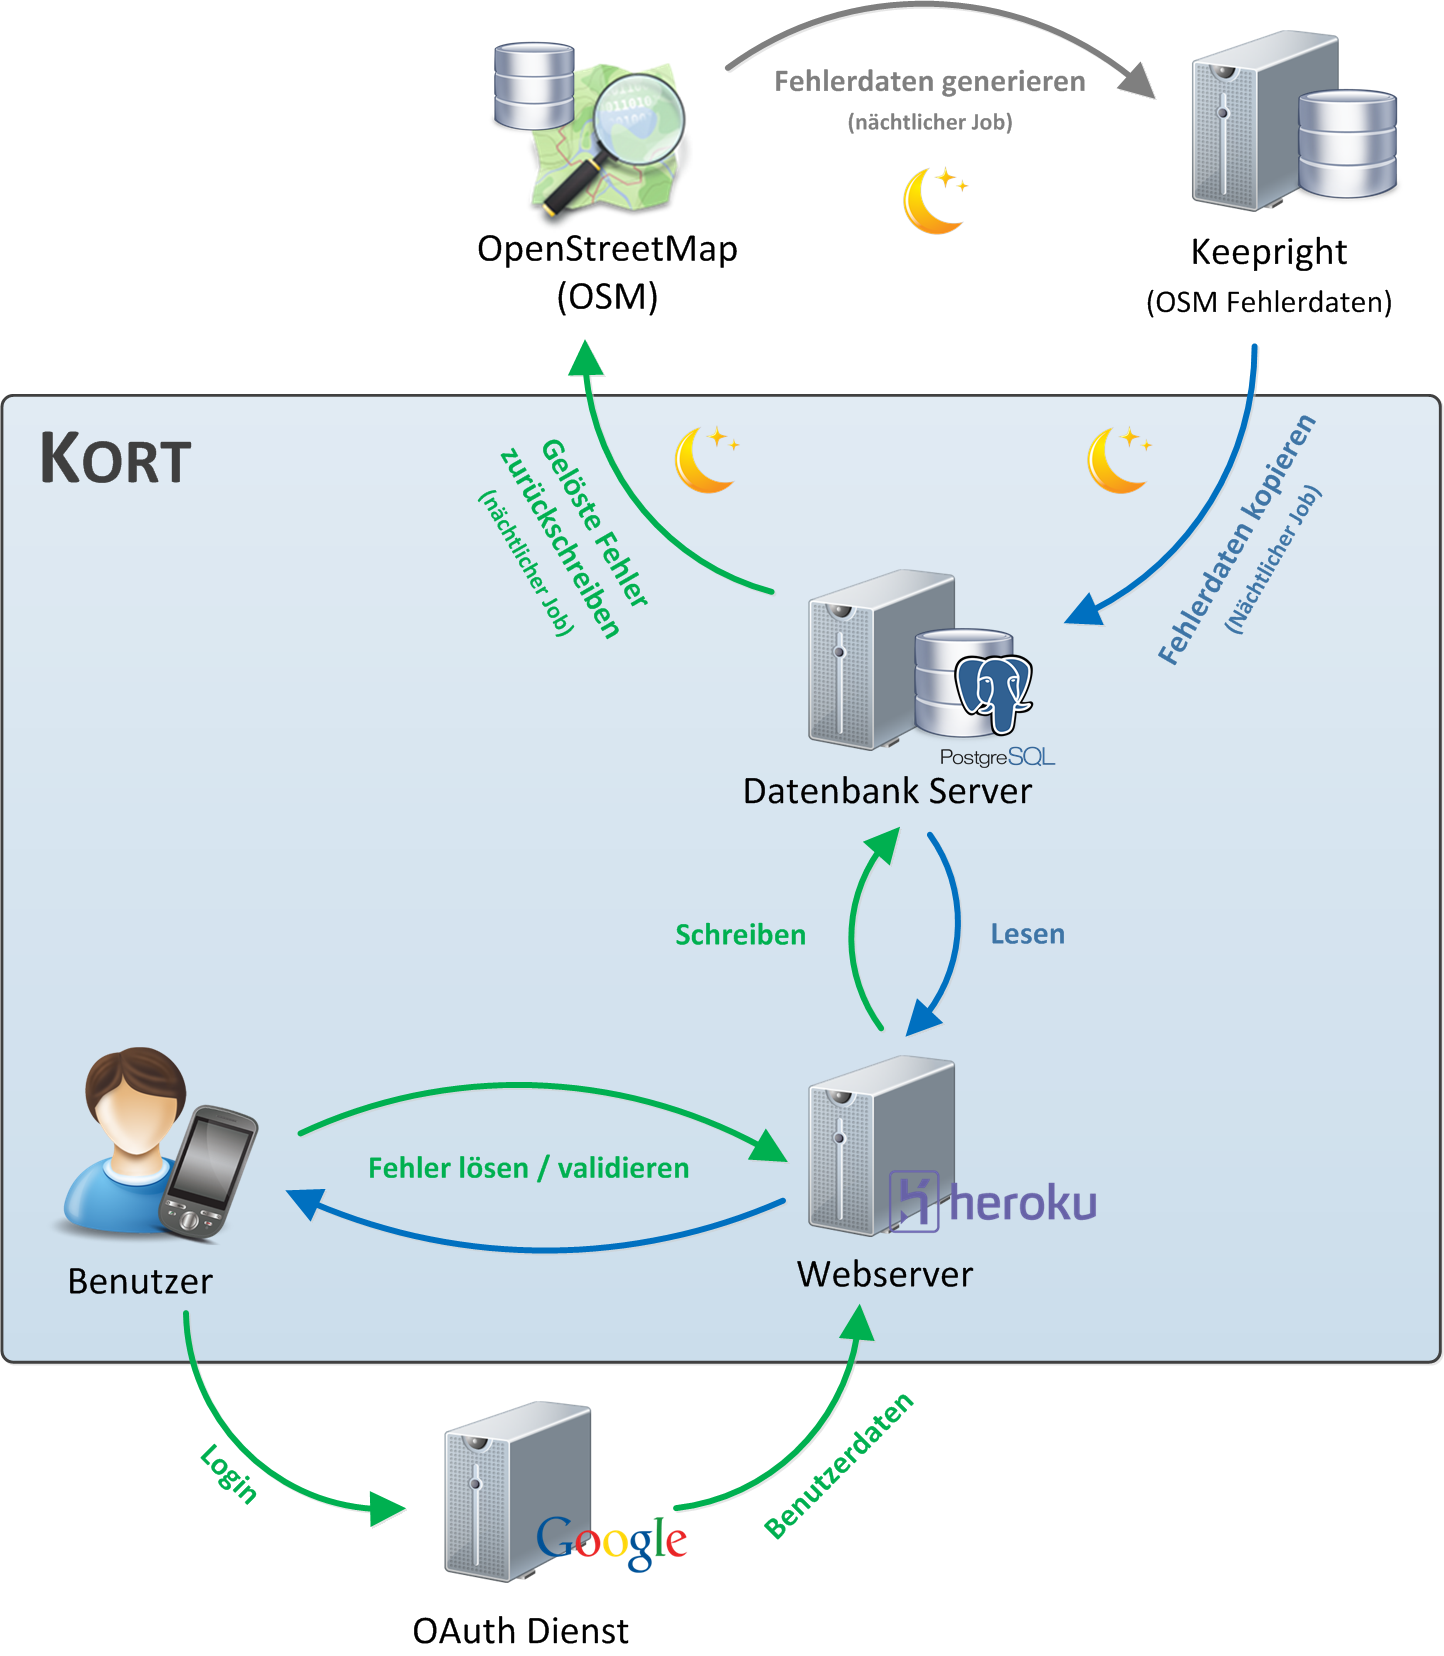
\includegraphics[scale=0.32]{images/implementation/backend/kort-big_picture}
	\caption{Übersicht des Gesamtsystems}
	\label{image-kort-big-picture}
\end{figure}

Das Backend besteht aus zwei logisch und derzeit auch physisch getrennten Servern. 
Der Webserver liefert die \gls{WebApp} aus und ist auch der einzige Kommunikationspartner für das Frontend. Dies ist zum einen eine architektonische, zum anderen eine technische Entscheidung.

\begin{itemize}
\item Das Frontend muss sich nicht darum kümmern, woher es welchen Dienst bezieht
\item Die Same-Origin-Policy\cite{sop} einiger Server lässt keine direkte Kommunikation zwischen \emph{fremdem} JavaScript und dem Server zu
\end{itemize}

Der Webserver ist somit der Dreh- und Angelpunkt der Applikation, jegliche Informationen von und zum Frontend durchläuft diese zentrale Komponente.

\begin{figure}[H]
	\centering
	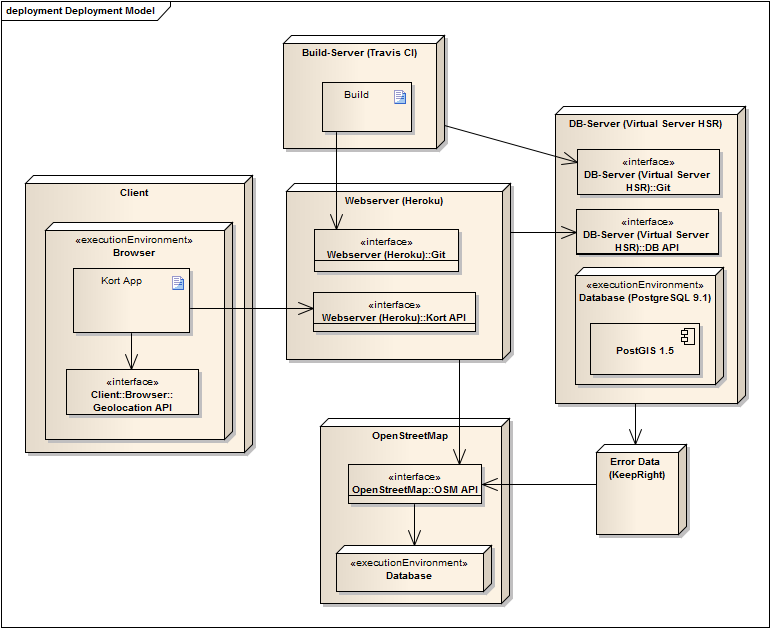
\includegraphics[width=\textwidth]{images/uml/deployment_diagram}
	\caption{Deployment-Diagramm}
	\label{deplyoyment-diagram}
\end{figure}

\section{Bootstrapping}
Das \gls{Bootstrapping} ist ein sehr wichtiges Grundprinzip dieser Arbeit.
Es besagt, dass sich das System selbst aufbauen kann.
Konkret haben wir darauf geachtet, dass für alle Aktionen Skripte oder Build-Schritte vorhanden sind, um diese später nachzuvollziehen.
Das Ziel ist es, ein System zu entwickeln, dass sich möglichst einfach wieder aufbauen lässt.

Auf der Seite des Datenbankservers geschieht dies so, dass die Datenbank jede Nacht neu aufgebaut wird.
Zum einen werden dabei die neuesten Fehlerdaten von \brand{KeepRight} geladen, zum anderen alle Änderungen an der Datenbank nachvollzogen.
Dies hat den grossen Vorteil, dass stets ein konsistenter Zustand anzutreffen ist.

Eine Ausnahme bilden dabei die laufenden Daten der Applikation (d.h. Userdaten, Lösungsvorschläge etc.), welche nicht jede Nacht zurückgesetzt werden.
Dies hat aber eher praktische als technische Gründe.

Auf der Seite des Webservers ist das \gls{Bootstrapping} noch stärker anzutreffen, da bei jedem Build das System komplett neu aufgebaut wird.
Somit müssen alle Informationen in Skripten hinterlegt sein, da sie sonst schlicht nicht zur Anwendung kommen.

\section{Umsysteme}
Zu unserem System gehören auch die Fehlerdatenquelle \brand{KeepRight} sowie \brand{OpenStreetMap} dazu.
Unsere Applikation interagiert direkt mit diesen beiden Systemen, ohne eine Kontrollfunktion zu übernehmen.
Es handelt sich somit um sogenannte Fremdsysteme.

Bei der Gestaltung der Systemlandschaft war es uns wichtig, diese so flexibel und offen wie möglich zu halten.
Weitere Systeme sollen sich einfach einbinden lassen.
Um dieses Ziel zu erreichen, haben wir darauf geachtet keine festen Verbindungen zwischen den Systemen zu schaffen.
Solche lassen sich später nur schwer wieder entfernen oder ändern.

Ein wichtiger Eckpfeiler ist es auch, die gesamte Kommunikation über \gls{REST}-Schnittstellen zu realisieren.
Dadurch lassen sich Dienste sowohl orts-, wie auch technologie-unabhängig voneinander betreiben.

\subsection{KeepRight}
Die Verbindung zu \brand{KeepRight} ist sehr lose, da das angebotene \gls{API} lediglich ein täglich generierter Dump von Fehlerdaten ist.
Diese Daten werden jede Nacht heruntergeladen und in unsere Datenbank integriert.

Weitere Fehlerquellen lassen sich einfach einbinden (siehe Abschnitt \ref{additional-error-source}), da innerhalb der Applikation nur über eine View auf die Daten zugegriffen wird.

\subsection{OpenStreetMap}
Das System benötigt drei Schnittstellen zu \brand{OpenStreetMap}, wovon in dieser Arbeit zwei realisiert sind.

\brand{OpenStreetMap} liefert die genauen Informationen über ein geografisches Objekt, um dieses auf einer Karte zeichnen zu können.
Dies verwenden wir, um Details zu einem Fehler anzuzeigen.
Wenn beispielsweise der Name einer Strasse erfasst werden soll, kann sich der Benutzer vorher über die Detail-Karte vergewissern, welche Strasse genau gemeint ist.

Der zweite Dienst, den wir beanspruchen, ist die Authentifizierung über \gls{OAuth}.
So kann das \brand{OpenStreetMap}-Benutzerkonto direkt verwendet werden, um \kort{} zu spielen.

Um den Kreis zu schliessen, sollen Korrekturen an \brand{OpenStreetMap} zurückgeschickt werden.
Dieses Themengebiet ist sehr heikel, da die \brand{OpenStreetMap}-Community technischen Benutzern sehr kritisch gegenübersteht\footnote{\url{http://lists.openstreetmap.org/pipermail/talk/2011-May/058396.html}}.
Es gilt die Grundregel, dass alle Änderungen über persönliche Benutzerkonten gemacht werden müssen.

Dies hat vor allem damit zu tun, dass Änderungen dadurch leichter nachvollziehbar sind.
Solche Einschränkungen können jedoch auch ein Hindernis sein.
In begründeten Fällen wird deshalb auch eine Ausnahme zugelassen.
Beispielsweise hat die \brand{WheelMap}-Applikation\footnote{\url{http://wheelmap.org/}} offiziell die Erlaubnis, mit einem technischen Benutzer Änderungen zu erfassen\footnote{\url{http://wiki.openstreetmap.org/wiki/Talk:Wheelmap}}.

Dies war unter anderem auch der Grund, weshalb wir unser Projekt am OSM-Stammtisch in Zürich vorgestellt haben\footnote{\url{http://wiki.openstreetmap.org/wiki/DE:Switzerland:Z\%C3\%BCrich/OSM-Treffen\#36._OSM-Stammtisch}}.
Das Feedback war durchaus positiv, jedoch gab es starke Vorbehalte gegenüber unserem Vorhaben, die korrigierten und validierten Lösungen automatisiert an \brand{OpenStreetMap} zu senden.

Das Thema ist also sowohl technisch und organisatorisch als komplex einzustufen.
Dies war uns von Anfang an klar, weshalb wir diesen Punkt auch in unserem Risikomanagement (siehe Abschnitt \ref{risikomanagement}) behandelt haben.
Schlussendlich hat uns die Zeit gefehlt, dieses Feature zu implementieren, weshalb \kort{} derzeit ein geschlossenes System ist, welches Lösungvorschläge für Fehlerdaten sammelt.

\section{Authentifizierung}
Bei jeder Applikation, welche Daten für verschiedene Nutzer speichert, stellt sich die Frage, wie sich die User anmelden sollen.
Die wichtigsten Kriterien dabei sind:

\begin{itemize}
\item Sicherheit
\item Einfachheit
\item Zielpublikum
\item Benötigte Zusatzdienste
\end{itemize}

Auf diese Kriterien hin, war für uns sofort klar, dass wir keine eigene Benutzerverwaltung machen wollten.
Ein App, das primär eine Ablenkung für einige Minuten sein soll, kann es sich nicht leisten, den Benutzer durch die Eingabe von Anmeldedaten abzuschrecken.

Daneben hat ein Benutzer bereits sehr viele Benutzerkonten bei verschiedensten Diensten.
Daher ist es auch naheliegend, diese Daten wiederzuverwenden.
Der Benutzer erspart sich dadurch ein weiteres Login, an das er sich erinnern muss.

\Gls{OAuth} ist mittlerweile ein gängiger Standard, um Applikationen Zugriff auf fremde Resourcen zu geben, ohne direkt den Benutzernamen und das Passwort preiszugeben.
Auch \brand{OpenStreetMap} unterstützt \gls{OAuth} und so fiel die Entscheidung leicht, dieses Protokoll zu verwenden.

In unserem Fall ist die Resource jedoch "`nur"' die Benutzerinformationen.
Das Protokoll basiert darauf, dass sowohl die Applikation, sowie der Benutzer dem jeweiligen \gls{OAuth}-Anbieter vertraut.

Vom authentisierten Benutzer werden dann die Benutzerinformationen (Name, ID, E-Mail) in unsere Datenbank übernommen.
Jeder Benutzer erhält daraufhin ein sogenanntes \emph{secret}, welches ihm fortan erlaubt, ohne erneuten Login die App zu nutzen.
Eine genaue Erklärung des Login-Ablaufs wird in Abschnitt \ref{oauth} beschrieben.

\section{REST}
\GLS{REST} ist die Idealvorstellung von plattformunabhängigen Schnittstellen.
So lassen sich alle möglichen Entitäten als \emph{Resourcen} darstellen, welche über eine der vier Grundfunktionalitäten (CRUD\cite{crud} - \inlinecode{Create}, \inlinecode{Read}, \inlinecode{Update}, \inlinecode{Delete}) manipuliert werden können.

Jede grössere Applikation kann von dieser Flexibilität profitieren.
Sie ermöglicht es, dass Funktionalitäten mit beliebigen Technologien und Programmiersprachen entwickelt werden können.
Dies ist besonders gut umsetzbar, wenn die Applikation bereits in Betrieb ist.
So können einzelne Komponenten neu entwickelt und in das bestehende System integriert werden, ohne eine nennenswerte Downtime.

Beim \gls{Marshalling} der Daten mag es effizientere Möglichkeiten geben als JSON\cite{json} und XML\cite{xml}.
Wenn die Datenmengen gering sind, fällt dies jedoch nicht stark ins Gewicht.
Sobald Binärdaten übertragen werden müssen, könnte es sinnvoll sein, einige Komponenten über andere Schnittstellen anzusprechen.

In unserem System spielt das keine Rolle, da unsere Requests durchschnittlich 10KB gross sind.


% Infrastruktur
\chapter{Infrastruktur}
\label{infrastruktur}

\section{Datenbankserver}

Beim Datenbankserver handelt es sich um einen virtuellen Server, den uns die HSR Hochschule für Technik Rapperswil für die Dauer dieser Arbeit zur Verfügung gestellt hat.
Dieser Server enthält die Installation der \kort{}-Datenbank sowie das Projektmanagementtool Redmine.
Letzteres ist die einzige kritische Anwendung auf dem Server, da sich der Rest über entsprechende Installationskripts sehr einfach und schnell neu aufbauen lässt.

Die Installation der benötigten Software kann mit dem Ubuntu Standard-Mechanismus \inlinecode{apt-\\get install} durchgeführt werden.

\begin{table}[H]
\centering
\begin{tabular}{|p{0.25\twocelltabwidth}|p{0.75\twocelltabwidth}|}
\hline 
\small{\textbf{Name}} & sinv-56055.edu.hsr.ch \\
\hline
\small{\textbf{DNS CNAME}} & kort.rdmr.ch \\
\hline 
\small{\textbf{Art des Servers}} & Virtueller Server \\
\hline 
\small{\textbf{Betriebsystem}} & Ubuntu 12.04 (LTS) \\
\hline 
\small{\textbf{Zugriff}} & Root-Zugriff via SSH \\
\hline 
\small{\textbf{Installierte Software}} & PostgreSQL 9.1, PostGIS 2.0, Redmine 2.1, MySQL 5.5, Apache Websever mit PHP 5.4 \\
\hline 
\small{\textbf{Pfade}} & Repository: \inlinecode{/home/odi/kort} \newline
Redmine: \inlinecode{/home/redmine/redmine-2.1.0} \\
\hline 
\end{tabular} 
\caption{Datenbankserver}
\label{infrastruktur-datenbankserver-tabelle}
\end{table}

\subsection{Datenbank-Webservice}
Der Zugang auf die Datenbank von aussen läuft ausschliesslich über den \gls{REST}-Webservice.
Für den Betrieb dieses Dienstes ist eine Apache Webserver Installation mit PHP-Unterstützung (mindestens PHP 5.3) erforderlich.

Für den Betrieb des Webservice ist das \kort{}-Repository auf dem Server geklont.
Anschliessend muss noch ein Symlink angelegt werden, um das Skript korrekt aufrufen zu können:

\inlinecode{\$ ln -s /home/odi/kort/server/webservices /var/www/webservices}

Der Webservice wird in Abschnitt \ref{webservice-database} genauer beschrieben.

\subsection{Redmine}
Die Installation von Redmine verlangt es, einen neuen Benutzer \inlinecode{redmine} auf dem Server anzulegen.
Danach muss die Software nur noch auf den Server kopiert werden und der Installationsanleitung gefolgt werden.
Diese ist in der Datei  \inlinecode{/server/redmine/redmine\_install.md} zu finden.

\subsubsection{Backup}
Die Daten von Redmine werden über zwei Skripts täglich gesichert. 
Das Skript \inlinecode{redmine\_\\backup.sh} kümmert sich darum, alle Backup-Daten täglich auf dem virtuellen Server zu sammeln und an einem zentralen Ort zu speichern.

Mit dem zweiten Skript \inlinecode{sync\_backup.sh} kann dann das zuvor erstellte Backup auf beliebige andere Systeme verteilt werden.
In unserem Fall haben wir das Skript auf unseren Laptops eingerichtet und so täglich die aktuellen Daten gesichert.


\section{Webserver (Heroku)}

Bei \brand{Heroku}\footnote{\url{http://www.heroku.com/}} handelt es sich um einen kostenlosen Dienst, welcher eine Deploymentumgebung für verschiedenste Plattformen anbietet. 
Der Dienst hat eine Schnittstelle, über welche sich automatisiert Applikationen erstellen lassen. Die Datenübertragung läuft dann über \gls{Git}.

\begin{table}[H]
\centering
\begin{tabular}{|p{0.25\twocelltabwidth}|p{0.75\twocelltabwidth}|}
\hline 
\small{\textbf{Art des Servers}} & Server in der \gls{Cloud} \\
\hline 
\small{\textbf{Betriebsystem}} & Ubuntu \\
\hline 
\small{\textbf{Zugriff}} & Daten via \gls{Git}, Befehle via Kommandozeilen-\gls{API} (\brand{Heroku-Toolbelt}) \\
\hline 
\small{\textbf{Installierte Software}} & Apache, \kort{} \gls{WebApp} \\
\hline 
\end{tabular} 
\caption{Server bei Heroku}
\label{infrastruktur-heroku-tabelle}
\end{table}

Die Entscheidung, den Webserver von \brand{Heroku} zu wählen, ist dadurch begründet, dass uns dies die grösstmögliche Freiheit bietet. 
\brand{Heroku} bietet bereits eine hervoragende \gls{API}, welche sich über das Kommandozeilen-Toolset \brand{Heroku-Toolbelt} steuern lässt.
Dies erlaubt es, beliebig viele Applikationen automatisiert zu erstellen.
Auch für den Betrieb bietet das \gls{API} viele Möglichkeiten zur Fernwartung an (SSH-Zugang, Logs, Prozessorauslastung).

\section{Deployment}
Am Deployment der Applikation sind mehrere Systeme beteiligt. 
Alle Änderungen werden von den Entwicklern via \gls{Git} zu \brand{GitHub}\footnote{\url{http://github.com}} übertragen. 
Auf \brand{GitHub} gibt es sogenannte \emph{Hooks}, die man aktivieren kann. 
Dabei handelt es sich um weitere Aktionen, welche durch verschiedene Ereignisse ausgelöst werden können. 
In unserem Fall haben wir einen \emph{post-commit Hook} aktiviert, welcher dem \gls{ci} Dienst \brand{Travis-CI}\footnote{\url{http://travis-ci.org}} Bescheid gibt, wenn neue Änderungen auf \brand{GitHub} eingetroffen sind.

Nach einem erfolgreichen Build werden die Resultate an \brand{Heroku} gesendet.
Zusätzlich wird der Datenbankserver über die Änderungen notifiziert, worauf dieser sich selbst aktualisiert.

\begin{figure}[H]
	\centering
	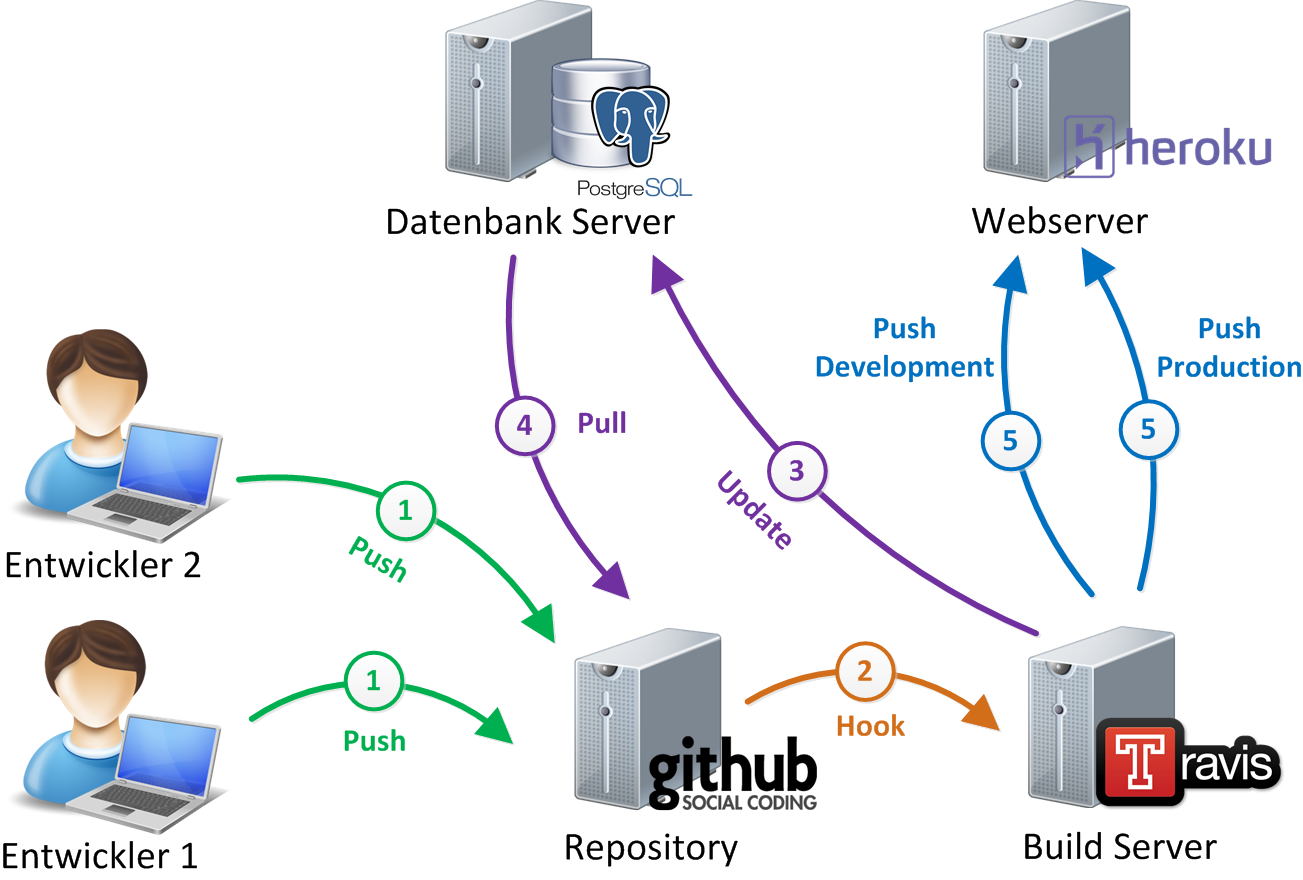
\includegraphics[scale=0.35]{images/implementation/backend/kort-development}
	\caption{Entwicklungsprozess von \kort{}}
	\label{image-kort-development}
\end{figure}

\subsection{Travis CI}
Auf \brand{Travis} läuft der Build, welcher durch die Konfigurationsdatei \inlinecode{.travis.yml} gesteuert ist. Darin lassen sich die Schritte sowie die Umgebung für Builds definieren.
Für jede Umgebung wird ein separater Build ausgelöst.
Somit lassen sich bequem verschiedene Versionen mit unterschiedlichen Umgebungen testen.
Daraus entsteht eine sogenannte Build-Matrix, welche bei jedem Build durchlaufen wird (siehe Tabelle \ref{infrastruktur-build-matrix}).

\begin{table}[H]
\centering
\begin{tabular}{|p{0.15\threecelltabwidth}|p{0.425\threecelltabwidth}|p{0.425\threecelltabwidth}|}
\hline 
 & \textbf{Test} & \textbf{Produktion} \\
\hline 
\textbf{PHP 5.3} & Build und Test & Build und Test \\
\hline 
\textbf{PHP 5.4} & Build, Test und Deployment auf \url{http://kort-dev.herokuapp.com} & Build, Test und Deployment auf \url{http://kort.herokuapp.com} \\
\hline 
\end{tabular} 
\caption{Build-Matrix von Travis CI}
\label{infrastruktur-build-matrix}
\end{table}

Ein Travis-Build läuft immer in einer neuen virtuellen Umgebung, so dass strikt nach dem Prinzip des \emph{\glslink{Bootstrapping}{Bootstrappings}} vorgegangen werden muss.
Das bedeutet, es muss möglich sein, die Applikation ohne Vorkenntnisse zu installieren.
Dies hilft, den Installationsprozess genau festzuhalten.

Am Ende des Build-Vorgangs wird die \gls{WebApp} schliesslich zu Heroku übertragen.

\subsection{Konfiguration über .travis.yml}
Die \inlinecode{.travis.yml} Datei ist die Konfigurationsdatei von \brand{Travis CI}.
Darin wird die Build-Matrix festgelegt sowie die die einzelnen Schritte des Builds definiert.

Vor dem eigentlichen Build wird die Umgebung aufgesetzt und die benötigte Software installiert (Zeilen 19-34 in Code-Ausschnitt \ref{travis-yml}).

\lstset{language=XML}
\begin{lstlisting}[float, caption=Die Travis CI Konfigurationsdatei .travis.yml, label=travis-yml]
language: php

php:
  - 5.3
  - 5.4

env:
  global:
    - CI_HOME=`pwd`/odi86/kort
    - DEPLOY="true"
    - BUILD_DIR=`pwd`/build_heroku
    - secure: "EIn+Rm7OxX8OKygBRBCaSTOqFGcBMWu5kHdKqSxOmHRJYjxuMOJpKV+rnyep\n+RsyFDx2Z9yKlqRRS4cpZh7M6wwC63EV46+7aWtzzTjnbMZfVzLQA9EmaEU4\nYMsKGtpQk2mhvaNKd3UbEpDl0Zq74NnAY0zipx0l02UymcFnZEc="
    - secure: "cOmMBP4UyklRC0nfeTZsX/NV4GhMBT+AntUmlWxXS5Rj2yrNcmNc7320gNm5\nCLSVRYyk7/8feyUEMznWrUn/62htZp0tEBAWtXg86dgIZgH4HPy9l2pKuSsH\nxZTHgjUJI7JOuyLG4ID9D5maVLE35UWag/NEtcRVy5QXLZOrs0M="
  matrix:
    - TARGET_ENV="dev"
    - TARGET_ENV="prod"

before_script:
  - gem install sass
  - gem install compass
  - gem install jsduck
  - wget -qO- https://toolbelt.heroku.com/install-ubuntu.sh | sh >/dev/null 2>&1
  - sudo npm install -g grunt >/dev/null 2>&1
  - pear install PHP_CodeSniffer && phpenv rehash
  - sudo pear channel-discover pear.survivethedeepend.com
  - sudo pear channel-discover hamcrest.googlecode.com/svn/pear
  - sudo pear channel-discover pear.phpdoc.org
  - sudo pear install --alldeps deepend/Mockery
  - sudo pear install phpdoc/phpDocumentor-alpha && phpenv rehash
  - sudo apt-get install graphviz
  - export PATH="$PATH:$CI_HOME:/usr/local/heroku/bin"
  - curl http://kort.rdmr.ch/webservices/update/git
  - mv $CI_HOME/server/php/Webservice/Database/DbConfig.example.php $CI_HOME/server/php/Webservice/Database/DbConfig.php

script: ant -f build_kort.xml build

after_script: bash $CI_HOME/server/heroku/heroku.sh
\end{lstlisting}

\subsubsection{Build-Matrix}
Die Build-Matrix bestimmt, welche Builds mit welchen Parametern ausgeführt werden.
Dabei wird gemäss definierten Sprachversionen (Zeilen 3-5 im Code-Ausschnitt \ref{travis-yml}) und Umgebungsvariablen (Zeilen 15-17) ein Build ausgeführt.
Daneben gibt es noch eine Reihe von globalen Umgebungsvariablen, welche in allen Builds verwendet werden.
In unserem Fall werden also vier Builds ausgeführt, mit jeweils PHP 5.3 und PHP 5.4 für die Test- und die Produktionsumgebung.

\subsubsection{Verschlüsselte Umgebungsvariablen}
Die Einträge mit \emph{secure} sind verschlüsselte Einträge, welche bei der Ausführung des Builds wieder entschlüsselt werden\footnote{\url{http://about.travis-ci.org/docs/user/build-configuration/\#Secure-environment-variables}}.
Auf diese Art lassen sich geheime Informationen wie \gls{API}-Schlüssel schützen.

In unserem \inlinecode{.travis.yml} kommt dies zweimal zum Einsatz:
\begin{enumerate}
\item \brand{Heroku} \gls{API}-Key, mit welchem sich beliebige Aktionen auf \brand{Heroku} durchführen lassen
\item \kort{} DB \gls{API}-Key, welcher den Datenbank-Webservice (siehe Abschnitt \ref{webservice-database}) vor fremden Zugriffen schützt
\end{enumerate}

\subsection{Apache Ant}
Das Build-Skript ist mit Apache Ant geschrieben.
Es beinhaltet alle Targets und Kombinationen davon, um einen kompletten oder teilweisen Build durchzuführen.

Derzeit werden bei einem vollständigen Build folgende Schritte durchlaufen:
\begin{enumerate}
\item Aus den SCSS-Quelldateien wird CSS generiert
\item Die JavaScript- und PHP-Dateien werden auf ihren Code Style geprüft
\item Anschliessend wird die Code-Dokumentation generiert
\item Zum Schluss werden noch die Unit Tests ausgeführt
\end{enumerate}

\subsubsection{GruntJS}
\label{gruntjs}
Die JavaScript spezifischen Build-Aufgaben werden von Ant an \brand{GruntJS}\footnote{\url{http://gruntjs.com/}} abgegeben.
Dieses Tool hat wiederum sein eigenes Konfigurationsfile \inlinecode{grunt.js}.
Darin sind Tasks beschrieben, welche auf den Code angewendet werden sollen.

In unserem Fall brauchen wir Grunt für zwei Aufgaben: JavaScript-Tests ausführen und JSHint auf sämlichen JavaScript Quellcode anwenden.

Bei \brand{JSHint}\footnote{\url{http://www.jshint.com/docs/}} handelt es sich um ein Linting-Werkzeug, welches mit diversen Optionen konfiguriert werden kann.
Das Ziel ist, dass der Code einheitlich wird und ein gewisser Code-Standard eingehalten wird.
Der Code wird dadurch besser lesbar und weniger fehleranfällig.

Die Unit Tests sind mit \brand{QUnit}\footnote{\url{http://qunitjs.com/}} erstellt und werden mit dem headless Browser \brand{PhantomJS}\footnote{\url{http://phantomjs.org/}} durchgeführt.
Dies ermöglicht es, auf einfache Art und Weise Frontend-Tests während dem Build durchzuführen.

\subsubsection{PHP\_CodeSniffer (PHPCS)}
\label{phpcs}
Der \brand{PHP\_CodeSniffer}\footnote{\url{http://pear.php.net/manual/en/package.php.php-codesniffer.php}} ist ein Linting-Tool für PHP.
Unser Code verwendet den Standard PSR-2\footnote{\url{https://github.com/php-fig/fig-standards/blob/master/accepted/PSR-2-coding-style-guide.md}}, welcher noch mit einigen Regeln zu PHPDoc-Kommentaren angereichert wurde.

Dadurch ist sichergestellt, dass der Code sauber ist und keine unerwarteten Seiteneffekte auftreten.
PHPCS lässt sich direkt in die Entwicklungsumgebung integrieren, so dass direkt beim Schreiben des Codes der Style überprüft werden kann.


% Backend
\chapter{Backend}
\label{backend}

% Implementation
\section{Implementation}
\label{backend-implementation}
Das Backend besteht neben der Datenbank und den \gls{REST}-Schnittstellen vor allem aus PHP-Code.
Der meiste Code entfällt auf das Handling von Webservice-Anfragen und die Authentifizierung mit \gls{OAuth}.

\subsection{Gliederung}
\label{backend-gliederung}
Das Backend befindet sich im Verzeichnis \inlinecode{server/} im Repository.
Das Backend teilt sich auf verschiedene Unterordner auf (siehe Tabelle \ref{table-backend-gliederung}).

\begin{table}[H]
\centering
\begin{tabular}{|p{0.25\twocelltabwidth}|p{0.75\twocelltabwidth}|}
\hline 
\textbf{Order} & \textbf{Inhalt} \\
\hline 
\inlinecode{database/} & SQL und Shell-Skripts für die Erstellung der Datenbank \\
\hline 
\inlinecode{heroku/} & Shell-Skripte für das Deployment auf Heroku \\
\hline 
\inlinecode{oauth2callback/} & Callback-Handler der verschiedenen \gls{OAuth}-Dienste \\
\hline 
\inlinecode{php/} & PHP-Klassen für das Backend \\
\hline 
\inlinecode{redmine/} & Skripts und Anleitung für Redmine \\
\hline 
\inlinecode{ssh\_pub\_keys/} & Öffentliche SSH-Schlüssel für das Deployment \\
\hline 
\inlinecode{webservices/} & \gls{REST}-Ressourcen (Endpunkte der Schnittstellen) \\
\hline 
\end{tabular}
\caption{Gliederung des Backends}
\label{table-backend-gliederung}
\end{table}

Speziell zu erwähnen sind dabei die PHP-Klassen, welche die Logik des Backends abbilden.
Sie sind über Namespaces aufgeteilt und liefern die Logik für alle anderen Teile des Backends.
Um dies zu ermöglichen, gibt es die \inlinecode{ClassLoader}-Klasse\footnote{\url{http://kort.herokuapp.com/docs/Kort-backend/classes/Kort.ClassLoader.html}}.
Falls irgendwo eine PHP-Klasse gebraucht wird, muss nur diese Klasse geladen werden, diese wiederum kümmert sich darum, alle abhängigen Dateien nachzuladen.

Für die Klassen gibt es eine separate Dokumentation (siehe Abschnitt \ref{backend-dokumentation}).

\subsection{Abhängigkeiten}
\label{backend-abhaengigkeiten}

\begin{table}[H]
\centering
\begin{tabular}{|p{0.35\threecelltabwidth}|p{0.15\threecelltabwidth}|p{0.50\threecelltabwidth}|}
\hline 
\textbf{Library} & \textbf{Version} & \textbf{Verwendung} \\
\hline 
Slim & 2.1.0 & Micro-Framework für die Implementation von \gls{REST}-Schnittstellen \\
\hline 
Google APIs Client Library & 0.6.0 & PHP-Library für Google \glspl{API} \\
\hline 
oauth-php & 175 & \gls{OAuth} Library für PHP \\
\hline 
Ant-Contrib & 1.0b3 & Erweiterte Tasks für Apache Ant \\
\hline 
\end{tabular}
\caption{Abhängigkeiten im Backend}
\label{table-backend-dependencies}
\end{table}



% REST Webservices
\section{REST-Schnittstellen}
Die Entscheidung, \gls{REST}-Schnittstellen zu verwenden, haben wir schnell gefasst. 
Zum einen ist damit eine einheitliche Schnittstelle im gesamten System vorhanden, so dass immer klar ist über welchen Kanal eine Kommunikation stattfindet.

Zum anderen sind \gls{REST}-Schnittellen für Webapplikation sehr einfach zu verwenden, da entsprechende Bibliotheksfunktionen bereits vorhanden sind.
Schlussendlich ist entscheidend, dass \gls{REST}-Schnittstellen ein grosses Mass an Plattformunabhängigkeit bieten und so die räumliche Teilung der Systeme erleichtern.

\subsection{Slim Framework}
Für die Erstellung der \gls{REST}-Webservices wurde das PHP Microframework \brand{Slim}\footnote{\url{http://www.slimframework.com/}} verwendet.
Das Framework ist sehr klein und beinhaltet nur das Nötigste, um die Webservices zu implementieren.
Bereits mit wenigen Zeilen Code lässt sich ein Webservice erstellen (siehe Code-Ausschnitt \ref{slim-example}).

\lstset{language=PHP}
\begin{lstlisting}[caption=Beispiel REST-Webservice in Slim, label=slim-example]
<?php
$app = new \Slim\Slim();
$app->get('/hello/:name', function ($name) {
    echo "Hello, $name";
});
$app->run();
\end{lstlisting}

% Webservice /answer
\input{body/projektdokumentation/backend/webservices/answer.tex}

% Webservice /bug
\input{body/projektdokumentation/backend/webservices/bug.tex}

% Webservice /highscore
\input{body/projektdokumentation/backend/webservices/highscore.tex}

% Webservice /osm
\input{body/projektdokumentation/backend/webservices/osm.tex}

% Webservice /user
\input{body/projektdokumentation/backend/webservices/user.tex}

% Webservice /user
\input{body/projektdokumentation/backend/webservices/validation.tex}

% Webservice /db
\input{body/projektdokumentation/backend/webservices/db.tex}

% Datenbank
\section{Datenbank}
Die Datenbank ist in verschiedenen Schemas organisiert.
Das Schema \inlinecode{kort} beinhaltet die Daten und Views für die Applikation.

\subsection{Views}Als Grundregel verwenden wir immer Views als \gls{API}, gegen das wir programmieren.
So lassen sich Änderungen daran sehr leicht einbringen, ohne dafür eine Tabelle anzupassen.

Jedes Model (siehe Abschnitt \ref{kort-store-model-package})  in der \gls{WebApp} hat seine eigene View in der Datenbank, welche genau die Daten liefert, welche es braucht.
Dies reduziert den Code für das Frontend und verschiebt die Datenlogik in die Datenbank.

\subsection{Applikationsschema}
Um die Applikationslogik möglichst von der Datenbank unabhängig zu halten, wird vom Backend-Code aus, lediglich auf die Views aus dem Schema \inlinecode{kort} zugegriffen.
Dadurch können weitere Schemas unabhängig voneinander hinzugefügt oder entfernt werden.
Auch Änderungen innerhalb des Schemas bedeuten keinen Bruch des View-\glspl{API}.

\subsection{Schema für Fehlerquellen}
Jede Fehlerquelle sollte ein eigenes Schema besitzen.
Jegliche Fehlerquellen-spezifischen Daten, Funktionen oder Types sind dann in diesem Schema gespeichert.
Dadurch lassen sich diese beliebig hinzufügen und entfernen.

In unserem Fall kommt uns das zugute, da jede Nacht das \brand{KeepRight} Schema gelöscht wird und anschliessend mit den neuen Fehlerdaten neu angelegt wird.

So ist sichergestellt, dass alle zugehörigen Informationen beieinander sind.
Lediglich in der View \inlinecode{kort.all\_errors} werden die Fehlerdaten der verschiedenen Schemas zusammengezogen.
Die Schemas für Fehlerquellen gehören somit nicht zum \gls{API} der Datenbank.

\subsection{Transaktionen}
Um die Konsistenz und Integrität der Daten zu wahren, war es eine wichtige Anforderung Transaktionen auf der Datenbank durchführen zu können.
So sollten beispielsweise einem Benutzer \emph{Koins} gutgeschrieben werden, wenn er einen Lösungsvorschlag abliefert.

Dadurch, dass die Datenbank über eine \gls{REST}-Schnittstelle angesprochen wird, könnte man auf die Idee kommen, mehrere Datenbankabfragen mit aufeinanderfolgenden Requests zu realisieren.
Dadurch könnte die Datenbank aber zwischen den einzelnen Requests in einen nicht-definierten Zustand geraten.

Um dies zu verhindern, ist es notwendig, Transaktionen über eine separate \gls{REST}-Ressource zu abstrahieren.
Clients können dazu ihre Abfragen in einem einzigen Request schicken. Diese werden dann in einer einzigen Datenbank-Transaktion ausgeführt (siehe Abschnitt \ref{webservice-database}).
Falls eine Abfrage schief läuft, werden automatisch die Änderungen der Transaktion rückgängig gemacht (\emph{Alles oder nichts}).

% Kommunikation
\section{Sicherheit}
\subsection{Authentifizierung mit OAuth}
\label{oauth}

Die Idee hinter \gls{OAuth} ist bestechend einfach: Eine Applikation möchte auf Dienste im Namen eines Benutzers zugreifen.
Der Benutzer möchte der Applikation sein Passwort jedoch nicht preisgeben, sondern lediglich einige wenige Ressourcen freigeben.
Da sowohl der Benutzer als auch die Applikation dem Anbieter der Ressource vertrauen, kann der Benutzer seinen Anbieter anweisen, der Applikation Zugriff zu gewähren.
Der Anbieter erstellt dazu ein sogenanntes \emph{Access Token}, welches er der Applikation zur Verfügung stellt.

Dieses Prinzip hat auf den ersten Blick nichts mit einem Login zu tun, jedoch kann das Vertrauensverhältnis des Benutzers zum Anbieter und der Applikation zum Anbieter dazu genutzt werden, einen Benutzer einzuloggen, ohne von ihm ein Passwort zu verlangen. 
Die Ressource beinhaltet in diesem Fall die verfügbaren Benutzerinformationen wie Namen, E-Mail Adresse oder ein Profilfoto.

\begin{figure}[H]
	\centering
	\includegraphics[scale=0.4]{images/implementation/backend/kort-login}
	\caption{Erster Login des Benutzers mit OAuth}
	\label{image-kort-login}
\end{figure}

In unserem Fall ist \kort{} die Applikation und \brand{Google} oder \brand{OpenStreetMap} der Anbieter der \emph{Benutzer}-Ressource.
Um dem Benutzer zu ersparen, sich bei jedem Besuch erneut via \gls{OAuth} anzumelden, wird auf dem Server ein \emph{Secret} generiert.
Dieses wird lokal beim Benutzer gespeichert (siehe Abbildung \ref{image-kort-login}) und ermöglicht es dem Benutzer beim nächsten Login direkt dieses \emph{Secret} zu übermitteln, um Zugriff auf die Applikation zu erhalten (siehe Abbildung \ref{image-kort-relogin}).
Diese Übertragung sollte wenn möglich über SSL/TSL erfolgen.

Wenn der Benutzer erfolgreich eingeloggt wurde, wird dies direkt in der Session des Benutzers gespeichert.
Auf die entsprechenden Werte wird dann bei sicherheitskritischen Abfragen zurückgegriffen.
So ist sichergestellt, dass ein Benutzer lediglich seine eigenen Daten manipulieren kann.

\begin{figure}[H]
	\centering
	\includegraphics[scale=0.4]{images/implementation/backend/kort-relogin}
	\caption{Wiedererkennen des Benutzers}
	\label{image-kort-relogin}
\end{figure}

\subsubsection{Registrierung der Applikation bei Google}
Um den Google \gls{OAuth} Dienst zu nutzen, muss diese zuerst registriert werden (siehe Abbildung \ref{image-oauth-google-settings}).
Ein Benutzer, der sich einloggen möchte, wird von \kort{} zu Google weitergeleitet.
Von dort wird er nach erfolgter Authentifizierung wieder zurückgeleitet.
Dieses "`Zurückleiten"' wird auch als \emph{Callback} bezeichnet.
Bei der Registrierung der Applikation müssen die gültigen Werte für den Callback definiert werden.

\begin{figure}[H]
	\centering
	\includegraphics[scale=0.5]{images/implementation/backend/oauth-google-settings}
	\caption{OAuth Einstellungen bei Google}
	\label{image-oauth-google-settings}
\end{figure}

\subsubsection{Registrierung der Applikation bei OpenStreetMap}
Die Registrierung bei \brand{OpenStreetMap} ist sehr ähnlich wie bei Google.
Leider bietet OSM aber keine Möglichkeit, bei einer Registrierung, mehrere URLs anzugeben.
Somit mussten wir für alle unsere Umgebungen (lokal, Entwicklung und Produktion) eine separate Registrierung vornehmen (siehe Abbildung \ref{image-oauth-osm}).

\begin{figure}[H]
	\centering
	\includegraphics[scale=0.5]{images/implementation/backend/oauth-osm}
	\caption{OAuth Einstellungen bei OpenStreetMap}
	\label{image-oauth-osm}
\end{figure}

\subsection{Übertragungssicherheit}
\label{uebertragunssicherheit}
Die App in der jetzigen Form bietet einige Angriffspunkte.
Die Übertragung über HTTP ermöglicht es einem Angreifer, Nachrichten mitzuhören.
Damit kann er theoretisch die Daten, welche von und zu der Applikation gesendet werden, abfangen und ändern.

Dies ist aus unserer Sicht aber kein grosses Problem, da es sich bei den Applikationsdaten weder um geheime noch besonders schützenswerte Informationen handelt.

Das grösste Risiko ist, dass es unerlaubte Zugriffe auf die Datenbank gibt.
Dazu müsste die Kommunikation zwischen dem Webserver und dem Datenbanksever abgefangen werden.
Der in jedem Request enthaltene \gls{API}-Key für die Datenbank läuft derzeit nicht ab.

Abhilfe würde hier eine Umstellung auf HTTPS (SSL/TLS) schaffen.
Dies erschwert das Mitlesen der Daten erheblich.
Des weiteren könnte die Kommunikation zwischen den Servern mit einem zeitlich generierten Token verbessert werden.
So können auch einfach Replay-Attacken verhindert werden.

Der Fokus dieser Arbeit lag aber nicht darauf, die Server-Server oder Server-Client Kommunikation sicher zu gestalten.
Für den produktiven Einsatz der Applikation müssen in diesem Bereich aber noch Verbesserungen erfolgen.

% Testing
\section{Testing}

\subsection{SimpleTest}
\brand{SimpleTest}\footnote{\url{http://simpletest.org/}} ist ein einfaches aber dennoch sehr flexibles Unit Testing Framework.
Die bestehende Funktionalität lässt sich sehr einfach erweitern und auf die eigenen Bedürfnisse anpassen.
Aus diesem Grund sind im Namespace \inlinecode{TestHelper}\footnote{\url{http://kort.herokuapp.com/docs/Kort-backend/namespaces/TestHelper.html}} einige Klassen entstanden als Erweiterung von SimpleTest.
So ist es beispielsweise möglich, die Tests sowohl im Browser, wie auch auf der Kommandozeile auszuführen.

Die Testresultate der Entwicklungsumgebung befinden sich unter \url{http://kort-dev.herokuapp.com/test}.

\begin{figure}[H]
	\centering
	\includegraphics[scale=0.5]{images/implementation/backend/simple-test}
	\caption{Testresultate von SimpleTest im Browser}
	\label{image-simple-test}
\end{figure}

Der derzeitige Build ist so konfiguriert, dass er fehlschlägt, wenn die Tests nicht bestanden werden.
Dies stellt sicher, dass sich nur stabile Versionen auf unserem Webserver befinden.

\cleardoublepage
\subsection{Integrationstests der Webservices mit QUnit}
Neben den klassischen Unit Tests, waren für die verschiedenen \gls{REST}-Webservices auch noch Integrationstest nötig.
Im Rahmen solcher Tests wird via \brand{QUnit} (welches wir für das JavaScript Testing benötigen) eine Anfrage an die betreffende Ressource gestellt.
Deren Antwort lässt sich dann im Unit Test leicht prüfen.

Die JavaScript Tests befinden sich auf der Entwicklungsumgebung unter \url{http://kort-dev.herokuapp.com/test/client/}.

\begin{figure}[H]
	\centering
	\includegraphics[width=\textwidth]{images/implementation/backend/qunit-skipped-test}
	\caption{Testresultate der Integrationstests im Browser}
	\label{image-qunit-skipped-test}
\end{figure}

% Dokumentation
% Dokumentation
\section{Dokumentation}

Das Frontend von \kort{} ist durchgängig mit der Sencha-eigenen Dokumentationssprache \brand{JSDuck}\footnote{\url{https://github.com/senchalabs/jsduck}} dokumentiert.
Die Dokumentation findet sich unter: \url{http://kort.herokuapp.com/docs/Kort}.

\begin{figure}[H]
	\centering
	\includegraphics[scale=0.33]{images/implementation/frontend/kort-documentation}
	\caption{Frontend Dokumentation mit JSDuck}
	\label{image-kort-documentation}
\end{figure}

% Administration
\chapter{Administration}
\label{administration}

\section{Hinzufügen von Fehler-Datenquellen}
\label{additional-error-source}
Die Applikation benutzt die View \inlinecode{kort.all\_errors} (siehe Abbildung \ref{image-kort-database-view-all_errors}) als Schnittstelle zu allen Fehlerdaten.
Wenn neue Fehlerquellen an das System angeschlossen werden sollen, dann muss entsprechend diese View angepasst werden.
Die aktuelle View ist auf die Fehlerquelle \brand{KeepRight} (siehe Kapitel \ref{datenquellen-keepright}) angepasst.

Es werden einige Anforderungen an eine neue Fehlerquelle gestellt:
\begin{itemize}
\item Ein Fehler muss sich konkret auf ein \brand{OpenStreetMap}-Objekt beziehen (\gls{Node}, \gls{Way} oder \gls{Relation})
\item Für die Darstellung auf der Karte muss eine einzelne Koordinate angegeben werden können (keine Flächen oder Wege)
\item Zu einem Fehler gibt es eine aussagekräftige Fehlermeldung
\end{itemize}

\begin{figure}[H]
	\centering
	\includegraphics[scale=0.7]{images/uml/kort-database-view-all_errors}
	\caption{Die View kort.all\_errors}
	\label{image-kort-database-view-all_errors}
\end{figure}

Die Fehler einer neuen Quelle müssen auf die bestehenden Fehlertypen gemappt werden.
Falls dies nicht möglich ist oder es sich um neue Arten von Fehlern handelt, müssen zusätzliche Fehlertypen eingeführt werden (siehe Abschnitt \ref{additional-error-type}).

Daneben müssen für alle neuen Fehlertypen Texte erfasst und allenfalls auch internationalisiert werden (siehe Abschnitt \ref{datenquellen-internationalisierung}).

\section{Hinzufügen von Fehlertypen}
\label{additional-error-type}
Um neue Fehlertypen hinzuzufügen müssen sowohl technische als auch fachliche Anpassungen vorgenommen werden.
Wichtig dabei ist es, den Endbenutzer nicht aus den Augen zu verlieren.
Alle aufgeführten Fehler sollten sich mit wenigen Eingaben lösen lassen.
Die bisher implementierten Fehlertypen benötigen alle nur eine einzige Eingabe.
Für neue Typen ist zu prüfen, ob diese sich bereits mit den bestehenden Views abbilden lassen (siehe Kapitel \ref{view-types}).
Ist dies nicht der Fall, so muss eine neue View erstellt werden.

\subsection{Fehlertypen}
In der Tabelle \ref{kort-bug-types-table} sind die in der App bereits implementierten Fehlertypen beschrieben.

\begin{table}[H]
\centering
\begin{tabular}{|p{0.40\twocelltabwidth}|p{0.37\twocelltabwidth}|}
\hline
\textbf{Fehlertyp} & \textbf{Anzahl vorhandener Fehler \newline \small{(Stand 20.12.2012)}} \\
\hline
Typ des Wegs unbekannt & 1'271'632 \\
\hline
Fehlendes Tempolimit & 463'819 \\
\hline
Sprache des Namens unbekannt & 111'565 \\
\hline
Objekt ohne Namen & 92'080 \\
\hline
Strasse ohne Namen & 74'864 \\
\hline
Kultstätte/Kirche ohne Religion & 15'288 \\
\hline
Autobahn ohne Bezeichner & 1'504 \\
\hline
\hline
\textbf{Total} & \textbf{2'030'752} \\
\hline
\end{tabular}
\caption{Fehlertypen in \kort{}}
\label{kort-bug-types-table}
\end{table}

Diese Typen sind in der Datenbanktabelle \inlinecode{kort.error\_type} (siehe Abbildung \ref{image-kort-database-table-error_type}) definiert.
Im Feld \inlinecode{type} dieser Tabelle befindet sich die eindeutige Identifikation eines Typs.
Diese wird beispielsweise für die Anzeige eines passenden Marker-Icons (auf der Karte) und der Verbindung zu einem passenden View-Typ (siehe Abschnitt \ref{view-types}) verwendet.

\begin{figure}[H]
	\centering
	\includegraphics[scale=0.7]{images/uml/kort-database-table-error_type}
	\caption{Die Tabelle kort.error\_type}
	\label{image-kort-database-table-error_type}
\end{figure}

\subsubsection{Erstellen eines neuen Fehlertyps}
\label{create-new-error-type}
Ein neuer Fehlertyp muss in der Tabelle \inlinecode{kort.error\_type} (siehe Abbildung \ref{image-kort-database-table-error_type}) hinzugefügt werden.
Sobald Fehler als \inlinecode{type} den neuen Typs eingetragen haben, wird dieser auch angezeigt.
Jeder Fehlertyp hat ein zugehöriges Marker-Icon, welches beispielsweise auf der Karte angezeigt wird.
Die Bilddatei hat den gleichen Namen wie das Attribut \inlinecode{type} und befindet sich im Ordner \inlinecode{resources/images/marker\_icons/<type>.png}.

\subsection{View-Typen}
\label{view-types}
All diese Typen werden dann wiederum einem spezifischen View-Typen zugeordnet.
Dieser bestimmt, wie das Formular zum Lösen des Fehlers in der Benutzeroberfläche aussieht.

In Tabelle \ref{kort-view-types-table} sind die bereits vorhandenen View-Typen beschrieben.

\begin{table}[H]
\centering
\begin{tabular}{|p{0.12\twocelltabwidth}|p{0.88\twocelltabwidth}|}
\hline
\textbf{Typ} & \textbf{Beschreibung} \\
\hline
\inlinecode{text} & Rendert ein Text-Eingabefeld \\
\hline
\inlinecode{number} & Rendert ein Zahl-Eingabefeld \\
\hline
\inlinecode{select} & Rendert eine Select-Box mit vorgefüllten Werten aus der Datenbank \\
\hline
\end{tabular}
\caption{View-Typen in \kort{}}
\label{kort-view-types-table}
\end{table}

Wird als View-Typ \inlinecode{select} gewählt, müssen in der Tabelle \inlinecode{kort.answer} (siehe Abbildung \ref{image-kort-database-table-answer}) die möglichen Antworten eingetragen werden.
Darin kann der eigentliche Wert des \brand{OpenStreetMap}-Tags und eine passende Bezeichnung hinterlegt werden.
Als \inlinecode{type} muss der jeweilige Typen-Bezeichner gewählt werden.

\begin{figure}[H]
	\centering
	\includegraphics[scale=0.7]{images/uml/kort-database-table-answer}
	\caption{Die Tabelle kort.answer}
	\label{image-kort-database-table-answer}
\end{figure}

\subsubsection{Erstellen eines neuen View-Typen}
Um einen neuen View-Typen zu definieren muss wie in Code-Ausschnitt \ref{code-kort-add_view_type} beschrieben die Unterscheidung in der Klasse \inlinecode{Kort.view.bugmap.fix.Form} mit dem den neuen Typen ergänzt werden.

\lstset{language=JavaScript}
\begin{lstlisting}[caption=Unterscheidung der View-Typen in Kort.view.bugmap.fix.Form, label=code-kort-add_view_type]
createFixField: function(bug) {
	[...]
	
	if(bug.get('view_type') === '<Neuer View-Typ>') {
		fixField = Ext.create('<Neue View-Klasse>', fieldConfig);
	} else {
		...
	}
	
	[...]
}
\end{lstlisting}

\section{Hinzufügen von Auszeichnungen}
\label{kort-additional-badges}
Die bereits vorhandenen Auszeichnungen sind in Tabelle \ref{kort-badges} beschrieben. Um weitere Auszeichnungen hinzuzufügen, muss folgendermassen vorgegangen werden:

\begin{enumerate}
\item Es muss ein neuer Badge in der Tabelle \inlinecode{kort.badge} (siehe Abbildung \ref{image-kort-database-table-badge}) erstellt werden
\item Zusätzlich muss eine Regel für das Gewinnen des Badges in der Methode \inlinecode{updateBadges()}\footnote{\url{http://kort.herokuapp.com/docs/Kort-backend/classes/Webservice.RewardHandler.html\#method_updateBadges}} der Klasse \inlinecode{RewardHandler} hinzugefügt werden.
\item Für das Frontend muss ein Bild erstellt werden, welches dem Namen (Tabellenattribut \inlinecode{name}) des Badges entspricht. Dieses Bild muss in folgendem Pfad gespeichert werden \inlinecode{/resources/images/badges/<badgename>.png}.
\end{enumerate}

\begin{figure}[H]
	\centering
	\includegraphics[scale=0.7]{images/uml/kort-database-table-badge}
	\caption{Die Tabelle kort.badge}
	\label{image-kort-database-table-badge}
\end{figure}

Sind alle Punkte abgearbeitet, ist der Badge im Frontend ersichtlich und kann von den Benutzern gewonnen werden.

\section{Hinzufügen von OAuth Anbietern}
\label{kort-additional-oauth-provider}
Derzeit ist der Login über die \gls{OAuth}-Dienste von \brand{OpenStreetMap} und \brand{Google} möglich. 
Um zukünftig weitere Login-Dienste anbieten zu können, müssen einige Schritte beachtet werden.
Der Dienst muss folgende Anforderungen erfüllen:
\begin{itemize}
\item Unterstützung für OAuth 1.0, 1.0a oder 2.0
\item Offline-Zugang, d.h. es müssen Aktionen ohne den Benutzer möglich sein
\item Der Dienst muss eine Registrierung der Applikation ermöglichen
\end{itemize}

Wenn ein Dienst diese Anforderung erfüllt, muss die Applikation registriert werden.

Im Backend kann eine entsprechende Subklasse von \inlinecode{AbstractOAuthCallback}\footnote{\url{http://kort.herokuapp.com/docs/Kort-backend/classes/OAuth.AbstractOAuthCallback.html}} erstellt werden. 
Eine so erstellte OAuthCallback-Klasse nimmt dann einen Callback des entsprechenden Anbieters entgegen und authentifiziert den Benutzer.
Das zugehörige Callback-Script wird im Order \inlinecode{/server/oauth2callback} gespeichert.

Schlussendlich muss das Frontend noch angepasst werden.
Dazu gehört, dass der neue Dienst in der Konfiguration (siehe Kapitel \ref{frontend-config}) eingetragen werden muss.
Um einen neuen Login-Button anzuzeigen, muss dieser auf dem Login-Panel hinzugefügt werden.
Die zugehörige Logik befindet sich im Login-Controller

Die Dateien befinden sich unter:
\begin{itemize}
\item Login-Panel: \inlinecode{/app/view/overlay/login/Panel.js}.
\item Login-Controller: \inlinecode{/app/controller/Login.js}
\end{itemize}

\begin{figure}[H]
	\centering
	\includegraphics[scale=0.5]{images/screenshots/kort-screenshot-login}
	\caption{Login-Buttons in \kort{}}
\end{figure}

\section{Reset der Applikation}
\label{kort-reset}
Um die Applikation zurückzusetzen, kann die Stored Procedure \inlinecode{reset\_kort()} verwendet werden. 
Die Prozedur löscht alle laufenden Daten aus der Datenbank, so dass wieder der Ursprungszustand hergestellt ist:
\begin{itemize}
\item Die Punkte (\emph{Koins}) aller Benutzer werden auf 0 zurückgesetzt
\item Die Badges aller Benutzer werden entfernt
\item Alle Lösungsvorschläge von Benutzern werden entfernt
\item Alle Überprüfungen von Lösungsvorschlägen werden entfernt
\end{itemize}

Der Aufruf der Prozedur sieht man im Code-Ausschnitt \ref{kort-reset-cmd}.
Die Prozedur liefert \inlinecode{true} wenn alle Aktionen erfolgreich ausgeführt werden konnten, ansonsten \inlinecode{false}.
\begin{lstlisting}[float, caption=Aufruf von reset\_kort(){,} um die Applikation zurückzusetzen, label=kort-reset-cmd]
select reset_kort();

 reset_kort 
------------
 t
(1 row)
\end{lstlisting}

\section{Frontend Konfiguration}
\label{frontend-config}
Die Konfiguration des Frontends befindet sich in der Datei \inlinecode{/app/util/Config.js}.
Darin sind alle Parameter definiert, welche die Applikation für den Betrieb benötigt.

In der \kort{}-Dokumentation sind alle Parameter detailliert beschrieben:

\url{http://kort.herokuapp.com/docs/Kort/#!/api/Kort.util.Config}


% Neue Seite beginnen
\cleardoublepage

% Projektmanagement
% Titel auch in Kopfzeile anzeigen
\markboth{Teil III. Projektmanagement und -monitoring}{Teil III. Projektmanagement und -monitoring}
\part{Projektmanagement und -monitoring}
% Projektmanagement
\chapter{Projektmanagement}
\label{projektmanagement}

Wir verwendeten die agile Projektmethodik \emph{Scrum}\footnote{\url{http://www.scrum.org}} und arbeiteten dabei während 14 Wochen.
Die Dauer eines Sprints haben wir auf 2 Wochen festgelegt.
In den ersten beiden Wochen waren wir mit dem Erstellen der Aufgabenstellung beschäftigt.
Für die restlichen 12 Wochen ergeben sich dadurch 6 Sprints.

\subsubsection{Aufwand pro Person}
Für diese Bachelorarbeit werden 12 ECTS-Punkte vergeben, wobei 1 ECTS-Punkt 30 Stunden Arbeitsaufwand bedeuten.
Dies ergibt 360 Stunden pro Person, was etwas mehr als 3 Arbeitstagen pro Woche entspricht.

\subsubsection{Anpassung der Sprintdauer}
Wir mussten während des Verlaufs des Projektes feststellen, dass die Sprintdauer von 2 Wochen etwas zu kurz ist und haben deshalb die letzten 6 Wochen mit 2 Sprints à 3 Wochen ersetzt.
Insgesamt wurden im Projekt 5 Sprints durchgeführt. 

\subsubsection{Storypoints pro Sprint}
Als Ausgangslage haben wir 12 Storypoints pro Sprint angenommen, wobei 1 Storypoint ungefähr einem Arbeitstag entspricht. 
Dieser Wert hat sich gut bewährt und wir mussten ihn lediglich bei der Anpassungen der Sprintdauer auf 17 Punkte erhöhen.

% Sprint 1
\cleardoublepage
\section{Sprint 1}

\textbf{1. Oktober 2012 bis 14. Oktober 2012}

Alle Informationen zum Sprint 1 sind auch in unserem Wiki zu finden:
\url{http://kort.rdmr.ch/redmine/projects/kort/wiki/Sprint_1}

\subsubsection{Hauptaufgaben / Fokussierung im Sprint}

\begin{itemize}
	\item Aufsetzen der Infrastruktur (Repository, Projektmanagement, Entwicklungsumgebung, Server)
	\item Einarbeitung in die Thematik
	\begin{itemize}
		\item \gls{Gamification}
		\item Highscore \gls{API}
		\item OpenStreetMap
		\item OpenLayers
		\item allenfalls weitere \glspl{API}
	\end{itemize}
	\item Wrapper für \brand{OpenStreetMap} in Sencha Touch
	\item Projektsetup
	\begin{itemize}
		\item GitHub\footnote{\url{http://www.github.com}} als Repository
		\item Heroku\footnote{\url{http://www.heroku.com}} fürs Hosting
		\item Travis\footnote{\url{http://travis-ci.org}} für Continuous Integration (CI)
		\item Redmine\footnote{\url{http://www.redmine.org}} für Projektmanagement/Wiki/Bugtracker
		\item \LaTeX{}\footnote{\url{http://www.latex-project.org}} für Dokumentation
		\item Scrum\footnote{\url{http://de.wikipedia.org/wiki/Scrum}} als Methodik
	\end{itemize}
\end{itemize}

\subsubsection{Ziele}
\begin{itemize}
	\item \brand{OpenStreetMap} genauer kennenlernen (Daten, Struktur, \gls{API})
	\item Integration in Sencha sicherstellen
\end{itemize}

\subsubsection{Abgabe / Deliverables}

\begin{itemize}
	\item Übersicht zum Projekt auf Redmine (Sprints, Issues/Tasks, generelle Infos)
	\item Projekt-Setup mit GitHub, Heroku und Jenkins
	\item Lauffähiger Prototyp mit \brand{OpenStreetMap} in Sencha Touch
\end{itemize}

\subsubsection{Erledigte Arbeiten}
Im ersten Sprint konnten wir bereits einiges erledigen. So gelang uns ein automatisierter Build der App inklusive Deployment zu Heroku. Ausserdem haben wir eine Sencha Touch Komponente für OpenLayers erstellt, um \brand{OpenStreetMap} Daten in der App darstellen zu können. Ebenfalls gelang es uns mit dem Plugin \brand{Ext.i18n.bundle-touch} die Internationalisierung der App vorzubereiten.

\subsubsection{Probleme}
Leider mussten wir feststellen, dass OpenLayers Library ein nicht mehr zeitgemässes \gls{API} aufweist. Es gilt deshalb im zweiten Sprint Alternativen dafür zu finden.

% Sprint 2
\section{Sprint 2}

\textbf{15. Oktober 2012 bis 28. Oktober 2012}

Alle Informationen zum Sprint 2 sind auch in unserem Wiki zu finden:
\url{http://kort.rdmr.ch/redmine/projects/kort/wiki/Sprint_2}

\subsubsection{Hauptaufgaben / Fokussierung im Sprint}

\begin{itemize}
	\item Alternative für OpenLayers finden
	\item Aufbau der Fehler-Datenbank
	\item Aufsetzen der REST-APIs für DB-Zugriff
	\begin{itemize}
		\item REST-API auf Heroku für Sencha-App
		\item REST-API auf DB-Server für Zugiff von Heroku
	\end{itemize}
	\item Requirements
	\begin{itemize}
		\item User Szenarien
		\item Paper Prototype
	\end{itemize}
\end{itemize}

\subsubsection{Ziele}
\begin{itemize}
	\item Roundtrip von Datenbank $\rightarrow$ Heroku $\rightarrow$ \gls{WebApp} und zurück (Daten lesen und schreiben)
	\item Anforderungen klar machen für Ausrichtung der App
	\begin{itemize}
		\item Was ist möglich?
		\item Was soll tatsächlich abgebildet werden?
	\end{itemize}
	\item Technische Hürden im Middletier überwinden, um sich auf Business-Logik und UI zu konzentrieren
\end{itemize}

\subsubsection{Abgabe / Deliverables}

\begin{itemize}
	\item Lauffähiger Prototyp
	\begin{itemize}
		\item Anzeigen von Bugs
		\item Eintragen von Daten in DB
	\end{itemize}
	\item User Szenarien
	\item Paper Prototyp
\end{itemize}

\subsubsection{Erledigte Arbeiten}
Während des zweiten Sprints haben wir verschiedene Fehler-Datenquellen evaluiert. Wir entschieden uns für den Einsatz der \brand{KeepRight}-Daten, da diese sehr gut unseren Anforderungen entsprechen. Sie werden automatisiert generiert, was es uns ermöglicht, für die verschiedenen Typen, auch automatisiert eine Lösungsmaske anzuzeigen. Zudem handelt es sich nur um Fehler in Tags der OpenStreetMap-Objekte.

Ebenfalls konnten wir, als Alternative zu OpenLayers, eine Sencha Touch Komponente erstellen, welche \brand{Leaflet} verwendet, um OpenStreetMap-Daten anzuzeigen.
Die Library besitzt ein gutes \gls{API} und wurde speziell für die Verwendung im mobilen Umfeld erstellt.

Schlussendlich konnten wir einen kompletten Roundtrip der Fehler-Daten von unserer Datenbank in die App und das Senden der Lösung wieder zurück in die Datenbank realisieren.

\subsubsection{Probleme}
Aus Zeitgründen konnten wir das Zurückschreiben der Daten zu \brand{OpenStreetMap} noch nicht erledigen.

% Sprint 3
\section{Sprint 3}

\textbf{29. Oktober 2012 bis 11. November 2012}

Alle Informationen zum Sprint 3 sind auch in unserem Wiki zu finden:
\url{http://kort.rdmr.ch/redmine/projects/kort/wiki/Sprint_3}

\subsubsection{Hauptaufgaben / Fokussierung im Sprint}

\begin{itemize}
	\item Backend
	\begin{itemize}
		\item Automatisierung der Fehlerdatenbank
		\item OAuth-Login bei Google/Facebook/Twitter etc.
	\end{itemize}
	\item Frontend
	\begin{itemize}
		\item Detail-Seiten für verschiedene Bug-Typen
		\item Profil-Seite
	\end{itemize}
\end{itemize}

\subsubsection{Ziele}
\begin{itemize}
	\item Welche Bug-Typen eignen sich für unsere App?
	\item Bug-Detailmasken implementiert
	\item OAuth Login und Logout
\end{itemize}

\subsubsection{Abgabe / Deliverables}

\begin{itemize}
	\item Lauffähiger Prototyp
	\begin{itemize}
		\item Anzeigen von Bug-Details (mind. 2 verschiedene Typen)
		\item Profile-Seite
		\item Login/Logout
	\end{itemize}
\end{itemize}

\subsubsection{Erledigte Arbeiten}
In diesem Sprint konzentrierten wir uns auf die Handhabung der verschiedenen Fehlertypen.
Wir mussten zuerst herausfinden, welche Typen sich für unsere App eignen.
Für diese mussten wir dann passende Lösungsmasken im Frontend erstellen.

Das zweite grosse Ziel war der Login bzw. Logout über OAuth. Dafür konnten wir ebenfalls eine erste Lösung erstellen.

\subsubsection{Probleme}
Der Benutzer wird derzeit noch nicht in der Datenbank persistiert. Der Login wird momentan noch nicht der Session gespeichert.

% Sprint 4
\section{Sprint 4}

\textbf{12. November 2012 bis 2. Dezember 2012}

Alle Informationen zum Sprint 4 sind auch in unserem Wiki zu finden:
\url{http://kort.rdmr.ch/redmine/projects/kort/wiki/Sprint_4}

\subsubsection{Hauptaufgaben / Fokussierung im Sprint}

\begin{itemize}
	\item Backend
	\begin{itemize}
		\item Datenbank-Setup
		\item OAuth-Handling auf Server (Refresh-Token)
	\end{itemize}
	\item Frontend
	\begin{itemize}
		\item Validations-Maske erstellen mit Fix-Einträgen, welche zu verifizieren sind
		\item Highscore-Masken
		\item Abschluss Bug Detailmasken
	\end{itemize}
\end{itemize}

\subsubsection{Ziele}
\begin{itemize}
	\item Validations-Maske implementiert
	\item Highscore-Maske implementiert
	\item Komplettes Datenbank-Setup
	\item User-Handling (Client, Server, Persistenz, Refresh-Token)
\end{itemize}

\subsubsection{Abgabe / Deliverables}

\begin{itemize}
	\item Lauffähiger Prototyp
	\begin{itemize}
		\item Validations-Maske zeigt zu validierenden Lösungsvorschläge an
		\item Highscore (global) kann angezeigt werden
		\item Datenbank mit vollständigem Schema (bootstrapped)
	\end{itemize}
\end{itemize}

\subsubsection{Erledigte Arbeiten}
Zu Beginn des Sprints mussten wir die Datenbank nach unserem definierten Schema aufbauen.
Dadurch konnten wir mit der Implementation der weiteren Masken der App (Validation, Highscore) starten.
Zusätzlich haben wir begonnen die Benutzeranmeldungen in der Datenbank zu persistieren.
Während dieses Sprints nahmen wir noch am OSM Stammtisch\footnote{\url{http://wiki.openstreetmap.org/wiki/DE:Switzerland:Z\%C3\%BCrich/OSM-Treffen\#36._OSM-Stammtisch}} teil und konnten dort unsere App der \glslink{Mapper}{Mapping}-Community präsentieren.
Wir erhielten spannende und wichtige Hinweise für die weitere Entwicklung unserer App.

\subsubsection{Probleme}
Leider konnten wir die Persistierung der Benutzer noch nicht komplett abschliessen.
Wir werden dies im nächsten Sprint angehen.

% Sprint 5
\section{Sprint 5}

\textbf{3. Dezember 2012 bis 21. Dezember 2012}

Alle Informationen zum Sprint 5 sind auch in unserem Wiki zu finden:
\url{http://kort.rdmr.ch/redmine/projects/kort/wiki/Sprint_5}

\subsubsection{Hauptaufgaben / Fokussierung im Sprint}

\begin{itemize}
	\item Fertigstellen der begonnenen Funktionalitäten
	\item Fehlerbehebungen
	\item Production-Build erstellen
	\item Dokumentation
	\begin{itemize}
		\item Code-Dokumentation
		\item Projektdokumentation
		\item A0 Poster erstellen
	\end{itemize}
\end{itemize}

\subsubsection{Ziele}
\begin{itemize}
	\item Abschliessen der begonnenen Funktionalitäten
	\begin{itemize}
		\item Gutschreiben der Koins / Badges
		\item Zurückschreiben der Daten zu OSM
		\item OAuth mit OpenStreetMap
	\end{itemize}
	\item Finalisieren der Dokumentation
\end{itemize}

\subsubsection{Abgabe / Deliverables}

\begin{itemize}
	\item Finale Version der App
	\item A0 Poster / Abstract / Management Summary
	\item Finale Version der Dokumentation
\end{itemize}

\subsubsection{Erledigte Arbeiten}

Im letzten Sprint lag der Fokus bei der Finalisierung der Applikation.
So mussten wir Funktionalitäten, welche noch nicht vollständig implementiert waren, fertigstellen und bestehende Fehler beheben.

An zusätzlichen Funktionen haben wir den Login über OpenStreetMap implementiert, sowie das Setzen des eigenen Benutzernamens auf der Profilseite.

Ebanfalls galt ein grosser Teil der Zeitplanung der Dokumentation des Projektes.

\subsubsection{Probleme}
Wir mussten aus Zeitgründen auf das Zurückschreiben der Korrekturen zu \brand{OpenStreetMap} verzichten.

% Projektmonitoring
\chapter{Projektmonitoring}
\label{projektmonitoring}

% Meilensteine
\section{Meilensteine}
\label{meilensteine}

Nachdem wir die Hauptaktivitäten des Projekts abschätzen konnten, haben wir eine Liste von Meilensteinen definiert.
Diese beschreiben konkrete Ziele welche während dieser Arbeit zu erreichen sind.

Wir haben uns jeweils einige Meilensteine für einen Sprint zum Ziel gesetzt und haben über die Wiki-Seite unseren Fortschritt festgehalten.

Somit gab es neben dem rein agilen Sprint-Planning auch noch funktionale Eckpfeiler.

\subsubsection{Meilenstein 1: Aufbereiten von Fehlerdaten}
\tick Geeignete Fehler finden \\
\tick Fehler in Datenbank speichern \\
\tick Fehler filtern \\
\tick Fehler zugänglich machen

\subsubsection{Meilenstein 2: Lesen von Fehlerdaten}

\tick Zugriff auf Datenbank aus App \\
\tick Persistieren der Daten in App

\subsubsection{Meilenstein 3: Kartenanzeige von Fehlern}

\tick Geeignete Darstellung der Fehler auf der Karte finden \\
\tick Fehler auf der Karte anzeigen \\
\tick Location-based Karte

\subsubsection{Meilenstein 4: OAuth}

\tick Login möglich über OAuth \\
\tick User wird in App persistiert \\
\tick Logout möglich \\
\tick Login mit OSM-OAuth

\subsubsection{Meilenstein 5: Schreiben von Fehlerbehebungen}

\tick Eingaben von Benutzer in DB speichern \\
\tick Unterscheidung von Fehlertypen

\subsubsection{Meilenstein 6: Validieren von Änderungen}

\tick UI zum Validieren von Fehlerbehebungen \\
\tick Implementation eines Thresholds für Validierung

\subsubsection{Meilenstein 7: Daten zu OSM schicken}

\cross Fehlerlösungen einheitlich via API an OSM senden \\
\cross Prüfung, ob eine Änderung zulässig ist

\subsubsection{Meilenstein 8: Gamification-Elemente}

\tick Geeignete Gamification-Elemente für OSM finden \\
\tick Elemente in App umsetzen

% Risikomanagement
\section{Risikomanagement}
\label{risikomanagement}

Für das Projekt wurden folgende Risiken identifiziert:
\subsection{Technische Risiken}

\subsubsection{OpenStreetMap-Daten können nicht in einer Sencha Touch-Applikation angezeigt werden}
\begin{table}[H]
\centering
\begin{tabular}{|p{0.25\twocelltabwidth}|p{0.75\twocelltabwidth}|}
\hline 
\small{\textbf{Auswirkung}} & Es müsste ein alternatives mobiles Framework gefunden werden, welches mit \brand{OpenStreetMap}-Daten umgehen kann. \\
\hline 
\small{\textbf{Wahrscheinlichkeit}} & tief \\
\hline 
\small{\textbf{Massnahme zur Verhinderung}} & Zu Beginn des Projektes muss eine Sencha Touch Prototyp-Applikation implementiert werden, welche \brand{OpenStreetMap}-Daten auf der Karte darstellt. \\
\hline
\end{tabular}
\end{table}

\subsubsection{Keine geeignete Fehlerdatenquelle vorhanden}
\begin{table}[H]
\centering
\begin{tabular}{|p{0.25\twocelltabwidth}|p{0.75\twocelltabwidth}|}
\hline 
\small{\textbf{Auswirkung}} & Es müsste eine Möglichkeit gefunden werden, vorhandene Fehlerdaten so abzuändern, dass sie für den Einsatz in der App verwendet werden können. \\
\hline 
\small{\textbf{Wahrscheinlichkeit}} & mittel \\
\hline 
\small{\textbf{Massnahme zur Verhinderung}} & Es muss eine Evaluation von bestehenden Fehlerdatenquellen durchgeführt werden. \\
\hline
\end{tabular}
\end{table}

\subsubsection{Schwierigkeiten mit OAuth}
\begin{table}[H]
\centering
\begin{tabular}{|p{0.25\twocelltabwidth}|p{0.75\twocelltabwidth}|}
\hline 
\small{\textbf{Auswirkung}} & OAuth ist als Protokoll bekannt, welches Schwierigkeiten bereiten kann.
Falls sich die Anforderungen nicht umsetzen lassen, muss eine alternative Lösung gefunden werden für den Login. \\
\hline 
\small{\textbf{Wahrscheinlichkeit}} & mittel \\
\hline 
\small{\textbf{Massnahme zur Verhinderung}} & Es muss genügend Zeit für OAuth eingeplant werden. \\
\hline
\end{tabular}
\end{table}

\subsection{Fachliche Risiken}

\subsubsection{OpenStreetMap erlaubt keinen allgemeinen Benutzer zum Zurückschreiben der Fehlerbehebungen}
\begin{table}[H]
\centering
\begin{tabular}{|p{0.25\twocelltabwidth}|p{0.75\twocelltabwidth}|}
\hline 
\small{\textbf{Auswirkung}} & Es müsste eine Möglichkeit gefunden werden, die Fehlerbehebungen trotzdem in \brand{OpenStreetMap} einpflegen zu können. \\
\hline 
\small{\textbf{Wahrscheinlichkeit}} & mittel \\
\hline 
\small{\textbf{Massnahme zur Verhinderung}} & \brand{OpenStreetMap}-Community muss von der Idee hinter \kort{} überzeugt werden. \\
\hline
\end{tabular}
\end{table}

\subsubsection{Zu wenig Erfahrung mit Game-Design}
\begin{table}[H]
\centering
\begin{tabular}{|p{0.25\twocelltabwidth}|p{0.75\twocelltabwidth}|}
\hline 
\small{\textbf{Auswirkung}} & Die App hat keinen Game-Charakter oder wird vom Benutzer nicht als solches erkannt. \\
\hline 
\small{\textbf{Wahrscheinlichkeit}} & gross \\
\hline 
\small{\textbf{Massnahme zur Verhinderung}} & Unser Industriepartner hat viel Erfahrung mit der Entwicklung von Games und kann uns mit Ratschlägen unterstützen.
Daneben haben wir versucht, Designer zu involvieren welche uns unterstützen können. \\
\hline
\end{tabular}
\end{table}

\section{Projektverlauf}
Das Projekt bestand aus 5 Sprints, wobei wir ursprünglich 6 geplant haben.
Gegen Ende des Projekts mussten wir uns eingestehen, dass der Overhead für zweiwöchige Sprints zu gross ist, deshalb haben wir die letzten beiden Sprints auf 3 Wochen erweitert.

Dank unserem Projektmanagement-Tool \brand{Redmine}, hatten wir eine gute Übersicht über das Projekt.
Jeweils am Ende eines Sprints haben wir besprochen, wie wir weiterfahren sollen und entsprechend den nächsten Sprint geplant.
Durch diese Iterationen war es uns möglich, schnell ein System zu erstellen, welches den aktuellen Bedürfnissen entspricht.

Abschliessend ist zu sagen, dass das Projekt gut verlaufen ist und wir grundsätzlich alle unsere Ziele erreichen konnten (siehe Abschnitt \ref{fazit}).
Daneben gab es auch Raum, kreative Ideen auszuprobieren.

\section{Arbeitsaufwand}
Wie im Kapitel \ref{projektmanagement} beschrieben, war der vom Modul vorgegebene Aufwand pro Person auf \emph{360 Stunden} festgelegt. Leider haben wir beide diese Vorgabe leicht überschritten (siehe Tabelle \ref{projektmanagement-arbeitsaufwand}).

\begin{table}[H]
\centering
\begin{tabular}{|l|l|}
\hline 
\textbf{Person} & \textbf{Aufwand} \\ 
\hline 
Jürg Hunziker & 379h \\
\hline 
Stefan Oderbolz & 394h \\  
\hline 
\end{tabular}
\caption{Arbeitsaufwand pro Person}
\label{projektmanagement-arbeitsaufwand}
\end{table} 

\section{Fazit}
\label{fazit}
Die entwickelte \gls{WebApp} erfüllt alle Erwartungen an eine moderne Applikation.
Ein Benutzer kann mit der App die gewünschten Aufgaben (Fehler korrigieren und validieren) durchführen und wird durch einige Gamification-Konzepte animiert, die App weiter zu verwenden.

In der knapp bemessenen Zeit ist es uns aber nicht gelungen ein vollwertiges Spiel zu entwickeln.
Dazu müsste noch mehr Wert auf Details gelegt werden, so dass ein abgerundetes Spielerlebnis entsteht.
Schlussendlich haben wir uns mehr auf die Grundfunktionalität der \gls{WebApp} konzentriert.

Mit Hilfe der \gls{ci} hatten wir stets ein lauffähiges System.
Dieses wurde bei jeder Änderung automatisiert neu gebaut und auf alle Systeme ausgerollt.

Dank der agilen Vorgehensweise konnten wir schnell auf Änderungen in den Anforderungen oder Probleme reagieren, welche sich bei einem solchen Projekt zwangsläufig ergeben.
Wir waren uns zu Beginn noch nicht bewusst, welche Funktionalitäten wichtig sind und welche weniger.
Der ursprüngliche Plan war, so schnell wie möglich den Roundtrip durch alle Systeme zu erfolgreich durchführen zu können.
Als wir aber erkannten, dass wir es mit vielen verschiedenen Schnittstellen zu tun haben, sind wir von diesem Plan wieder abgekommen und haben uns dazu entschlossen, zuerst unsere App zu stabilisieren und dann eine Schnittstelle nach der anderen anzuschauen.

Die Arbeit hat uns viele spannende Einblicke in \brand{OpenStreetMap} und die Thematik der \gls{Gamification} ermöglicht.
Das \brand{OpenStreetMap}-Umfeld ist sehr interessant und die intensive Arbeit mit Fehlerdaten hat uns gezeigt wie einzigartig dieses Projekt ist.

Wir hoffen, dass auch unsere App ihren Teil dazu beiträgt neue Benutzer fürs \glslink{Mapper}{Mappen} zu begeistern.

% -----------------------------------------
% FOOT
% -----------------------------------------
% Neue Seite beginnen
\cleardoublepage

% Anhänge
% Titel auch in Kopfzeile anzeigen
\markboth{Teil V. Anhänge}{Teil V. Anhänge}
\part{Anhänge}

% Inhalt der CD
\chapter*{Inhalt der CD}
% Titel auch in Kopfzeile anzeigen
\markboth{Inhalt der CD}{Inhalt der CD}
% Kapitel in Inhaltsverzeichnis einfügen
\addcontentsline{toc}{chapter}{Inhalt der CD}

\begin{table}[H]
\centering
\begin{tabular}{|p{0.35\twocelltabwidth}|p{0.65\twocelltabwidth}|}
\hline 
\textbf{Pfad} & \textbf{Beschreibung} \\ 
\hline 
\inlinecode{.sencha/} & Konfiguration für Sencha Cmd \\ 
\hline 
\inlinecode{\_DESIGN/} & Grafik-Rohdaten \\ 
\hline 
\inlinecode{\_DOCUMENTATION/} & Dokumentation der Arbeit \\ 
\hline 
\inlinecode{\_DOCUMENTATION/ba-kort-
\newline jhunzike\_soderbol.pdf} & Dokumentation der Arbeit im PDF-Format \\ 
\hline 
\inlinecode{app/} & \kort{} Frontend \\ 
\hline 
\inlinecode{build/Kort/production/} & \kort{} Production Build (komprimierte JavaScript Sourcefiles) \\ 
\hline 
\inlinecode{docs/} & Generierte Code-Dokumentationen (\kort{} Frontend, \kort{} Backend, Ext.ux.LeafletMap) \\ 
\hline 
\inlinecode{examples/} & Frontend Prototypen \\ 
\hline 
\inlinecode{i18n/} & Internationalisierungs-Plugin für Sencha Touch \\ 
\hline 
\inlinecode{jsduck/} & Konfiguration zur Generierung der JSDuck Code-Dokumentation \\ 
\hline 
\inlinecode{lib/} & Verwendete Library-Pakete \\ 
\hline 
\inlinecode{patch/} & Sencha Touch Bugfixes \\ 
\hline 
\inlinecode{resources/} & Ressourcen, welche von \kort{} verwendet werden (CSS, Bilder, Sprach-Property-Files) \\ 
\hline 
\inlinecode{server/} & \kort{} Backend \\ 
\hline 
\inlinecode{test/} & Tests der Applikation \\ 
\hline 
\inlinecode{touch/} & Sencha Touch 2 Library \\ 
\hline 
\inlinecode{ux/} & Sencha Touch Erweiterungs-Komponenten \\ 
\hline 
\inlinecode{.travis.yml} & Konfiguration für Travis CI \\ 
\hline 
\inlinecode{app.js} & Einstiegspunkt des \kort{} Frontends \\ 
\hline 
\inlinecode{app.json} & Sencha Cmd Konfiguration von \kort{} \\ 
\hline 
\inlinecode{index.html} & Startseite \\ 
\hline 
\end{tabular}
\end{table}

% Glossar
\printglossary[style=altlist,title=Glossar,toctitle=Glossar]
\label{glossar}

% Literaturverzeichnis
\bibliographystyle{plainurl}
\bibliography{foot/literatur}

% Abbildungsverzeichnis
\listoffigures

% Tabellenverzeichnis
\listoftables

\end{document}